%\documentclass{beamer}
%\documentclass[slidestop,usepdftitle=false]{beamer}
\documentclass[english,10pt,table]{beamer}
%\documentclass[english,10pt,table,handout]{beamer}
\usepackage{tikz}
\usepackage[english]{babel}
\usepackage[utf8]{inputenc}

\usepackage[utf8]{vietnam}
\usepackage{a4wide,amssymb,epsfig,latexsym,array,hhline,fancyhdr}
\usepackage[normalem]{ulem}
\usepackage{soul}
\usepackage{listings}

\usepackage[makeroom]{cancel}
\usepackage{amsmath}
\usepackage{amsthm}
\usepackage{diagbox}%Make diagonal lines in tables
\usepackage{booktabs}
\usepackage{alltt}
\usepackage[framemethod=tikz]{mdframed}% For highlighting paragraph backgrounds
\usepackage{caption,subcaption}
\usepackage{float}

\usepackage{lastpage}
\usepackage[lined,boxed,commentsnumbered]{algorithm2e}
\usepackage{enumerate}
\usepackage{color}
\usepackage{graphicx}							% Standard graphics package
\usepackage{array}
\usepackage{tabularx, caption}
\usepackage{multirow}
\usepackage{multicol}
\usepackage{rotating}
\usepackage{graphics}
\usepackage{geometry}
\usepackage{setspace}
\usepackage{epsfig}
\usepackage{tikz}
\usepackage{tcolorbox}
\usetikzlibrary{arrows,backgrounds}
\usepackage[unicode]{hyperref}
							% PSTricks with the standard color package
\usepackage[normalem]{ulem}
% Copyright 2007 by Till Tantau
%
% This file may be distributed and/or modified
%
% 1. under the LaTeX Project Public License and/or
% 2. under the GNU Public License.
%
% See the file doc/licenses/LICENSE for more details.


% Common packages

\usepackage[english]{babel}
\usepackage[utf8]{vietnam}
%\usepackage{times}
\usefonttheme[onlymath]{serif}
\usecolortheme{default}
\usepackage{booktabs}
\usepackage{mathpartir}
\usepackage{listings}
\usepackage{pbox}
\mprset{flushleft}
\mode<article>
{
  \usepackage{times}
  \usepackage{mathptmx}
  \usepackage[left=1.5cm,right=6cm,top=1.5cm,bottom=3cm]{geometry}
}

\usepackage{hyperref}
\usepackage{tikz}
\usetikzlibrary{arrows,backgrounds}
%\tikzstyle{mnode}=[circle, draw, fill=black, inner sep=0pt, minimum width=4pt]
\usepackage{colortbl}
%\usepackage{yfonts}
\usepackage{translator} % comment this, if not available


% Common settings for all lectures in this course

\def\lecturename{BTL CTRR}

\title{\insertlecture}

\author{Kim Gia Bao, Nguyen The Cuong, Le Nhat Anh, Do Nhat Thai}

\institute
{
  Faculty of Computer Science and Engineering\\
  University of Technology - VNUHCM 
}

\subject{Lecturer \lecturename}




% Beamer version theme settings

\useoutertheme[height=0pt,width=2cm,right]{sidebar}
\usecolortheme{rose,sidebartab}
\useinnertheme{circles}
\usefonttheme[only large]{structurebold}

\setbeamercolor{sidebar right}{bg=black!15}
\setbeamercolor{structure}{fg=blue}
\setbeamercolor{author}{parent=structure}

\setbeamerfont{title}{series=\normalfont,size=\LARGE}
\setbeamerfont{title in sidebar}{series=\bfseries}
\setbeamerfont{author in sidebar}{series=\bfseries}
\setbeamerfont*{item}{series=}
\setbeamerfont{frametitle}{size=}
\setbeamerfont{block title}{size=\small}
\setbeamerfont{subtitle}{size=\normalsize,series=\normalfont}
\setbeamerfont{block body}{size =\tiny,basicstyle=\tiny}
\lstset{basicstyle=\tiny}
\setbeamertemplate{navigation symbols}{}
\setbeamertemplate{bibliography item}[book]
\setbeamertemplate{sidebar right}
{
  {\usebeamerfont{title in sidebar}%
    \vskip1.5em%
    \hskip3pt%
    \usebeamercolor[fg]{title in sidebar}%
    \insertshorttitle[width=2cm,center,respectlinebreaks]\par%
    \vskip1.25em%
  }%
  {%
    \hskip3pt%
    \usebeamercolor[fg]{author in sidebar}%
    \usebeamerfont{author in sidebar}%
    \insertshortauthor[width=2cm,center,respectlinebreaks]\par%
    \vskip1.25em%
  }%
  \hbox to2cm{\hss\insertlogo\hss}
  \vskip1.25em%
  \insertverticalnavigation{2cm}%
  \vfill
  \hbox to 2cm{\hfill\usebeamerfont{subsection in
      sidebar}\strut\usebeamercolor[fg]{subsection in
      sidebar}\insertshortlecture.\insertframenumber\hskip5pt}%
  \vskip3pt%
}%

\setbeamertemplate{title page}
{
  \vbox{}
  \vskip1em
  {\huge Chapter \insertshortlecture\par}
  {\usebeamercolor[fg]{title}\usebeamerfont{title}\inserttitle\par}%
  \ifx\insertsubtitle\@empty%
  \else%
    \vskip0.25em%
    {\usebeamerfont{subtitle}\usebeamercolor[fg]{subtitle}\insertsubtitle\par}%
  \fi%     
  \vskip1em\par
  \emph{\lecturename}\ on \insertdate\par
  \vskip0pt plus1filll
  \leftskip=0pt plus1fill\insertauthor\par
  \insertinstitute\vskip1em
}

\logo{
\includegraphics[width=1.5cm]{Images/hcmut.png}}



% Article version layout settings

\mode<article>

\makeatletter
\def\@listI{\leftmargin\leftmargini
  \parsep 0pt
  \topsep 5\p@   \@plus3\p@ \@minus5\p@
  \itemsep0pt}
\let\@listi=\@listI


\setbeamertemplate{frametitle}{\paragraph*{\insertframetitle\
    \ \small\insertframesubtitle}\ \par
}
\setbeamertemplate{frame end}{%
  \marginpar{\scriptsize\hbox to 1cm{\sffamily%
      \hfill\strut\insertshortlecture.\insertframenumber}\hrule height .2pt}}
\setlength{\marginparwidth}{1cm}
\setlength{\marginparsep}{4.5cm}

\def\@maketitle{\makechapter}

\def\makechapter{
  \newpage
  \null
  \vskip 2em%
  {%
    \parindent=0pt
    \raggedright
    \sffamily
    \vskip8pt
    {\fontsize{36pt}{36pt}\selectfont Bài tập lớn \insertshortlecture \par\vskip2pt}
    {\fontsize{24pt}{28pt}\selectfont \color{blue!50!black} \insertlecture\par\vskip4pt}
    {\Large\selectfont \color{blue!50!black} \insertsubtitle\par}
    \vskip10pt

    \normalsize\selectfont Print version of
    Lecturer \emph{\lecturename} of \@date\par\vskip1.5em
    \hfill Tran Vinh Tan, Faculty of CSE, University of Technology
  }
  \par
  \vskip 1.5em%
}

\let\origstartsection=\@startsection
\def\@startsection#1#2#3#4#5#6{%
  \origstartsection{#1}{#2}{#3}{#4}{#5}{#6\normalfont\sffamily\color{blue!50!black}\selectfont}}

\makeatother

\mode
<all>




% Typesetting Listings

\usepackage{listings}
\lstset{language=Java}

\alt<presentation>
{\lstset{%
  basicstyle=\footnotesize\ttfamily,
  commentstyle=\slshape\color{green!50!black},
  keywordstyle=\bfseries\color{blue!50!black},
  identifierstyle=\color{blue},
  stringstyle=\color{orange},
  escapechar=\#,
  emphstyle=\color{red}}
}
{
  \lstset{%
    basicstyle=\ttfamily,
    keywordstyle=\bfseries,
    commentstyle=\itshape,
    escapechar=\#,
    emphstyle=\bfseries\color{red}
  }
}



% Common theorem-like environments

\theoremstyle{example}
\newtheorem{exercise}[theorem]{\translate{Exercise}}


% New useful definitions:

\newbox\mytempbox
\newdimen\mytempdimen

\newcommand\includegraphicscopyright[3][]{%
  \leavevmode\vbox{\vskip3pt\raggedright\setbox\mytempbox=\hbox{\includegraphics[#1]{#2}}%
    \mytempdimen=\wd\mytempbox\box\mytempbox\par\vskip1pt%
    \fontsize{3}{3.5}\selectfont{\color{black!25}{\vbox{\hsize=\mytempdimen#3}}}\vskip3pt%
}}

\newenvironment{colortabular}[1]{\medskip\rowcolors[]{1}{blue!20}{blue!10}\tabular{#1}\rowcolor{blue!40}}{\endtabular\medskip}

\def\equad{\leavevmode\hbox{}\quad}

\newenvironment{greencolortabular}[1]
{\medskip\rowcolors[]{1}{green!50!black!20}{green!50!black!10}%
  \tabular{#1}\rowcolor{green!50!black!40}}%
{\endtabular\medskip}




\lecture[0]{Bài tập lớn\\ môn Cấu Trúc Rời Rạc cho KHMT}{lecture-text}

\usepackage{pifont}
% Symbol definitions for these lists
\newcommand{\DingListSymbolA}{43}
\newcommand{\DingListSymbolB}{243}
\newcommand{\DingListSymbolC}{224}
\newcommand{\DingListSymbolD}{219}

% Boxed equation
\definecolor{LightYellow}{rgb}{1.,1.,.9}
\definecolor{LightRed}{rgb}{1.,.6,.6}


%%ensembles de nombres
\def\NP{$\mathcal{NP}$}
\def\N{\mathbb{N}}
\def\Z{\mathbb{Z}}
\def\R{\mathbb{R}}
\def\Q{\mathbb{Q}}

%\date[]{~~}
%%%%%%%%%%%%%%%%%%%%%%%%%%%%%%%%%%%%%%%%%%%%%%%%%%%%%%%%%%%%%%%%%%%%%
%%%%%%%%%%%%%%%%%%%%%%%%%%%%%%%%%%%%%%%%%%%%%%%%%%%%%%%%%%%%%%%%%%%%%
\begin{document}
\frame{
\selectlanguage{english}
  \maketitle
}

%%%%%%%%%%%%%%%%%%%%%%%%%%%%%%%%%%%%%%%%%%%%%%%%%%%%%%%%%%%%%%%%%%%%%
%%%%%%%%%%%%%%%%%%%%%%%%%%%%%%%%%%%%%%%%%%%%%%%%%%%%%%%%%%%%%%%%%%%%%
%\section[Plan]{}
%\setcounter{tocdepth}{1}
\frame{ \tableofcontents}
%\setcounter{tocdepth}{5}
% to display left summary deeper and plan slide juste display section: add command \setcounter{tocdepth}{1} and then \setcounter{tocdepth}{10}  recompile twice or more again 

%%%%%%%%%%%%%%%%%%%%%%%%%%%%%%%%%%%%%%%%%%%%%%%%%%%%%%%%%%%%%%%%%%%%%
%%%%%%%%%%%%%%%%%%%%%%%%%%%%%%%%%%%%%%%%%%%%%%%%%%%%%%%%%%%%%%%%%%%%%
\section{Động cơ nghiên cứu}
\frame
{
  \frametitle{1. Động cơ nghiên cứu}	
Bệnh Corona do virus gây ra còn gọi là COVID-19 đã tạo ra những tác động tiêu cực đến nền đời
sống của cư dân trên thề giới. Các đợt bùng phát của COVID-19 hay những biến thể virus đã mang đến
những thách thức chưa từng có và được dự báo sẽ có tác động đáng kể đến sự phát triển kinh tế. Nhiều
thông tin, tin tức về tình hình dịch bệnh cũng như dữ liệu về COVID-19 được phổ biến rộng rải trong
đời sống hay trên internet để giúp cho mọi người quan sát, phân tích, nghiên cứu đươc cập nhật hàng
ngày.
}
\begin{frame}
\frametitle{1. Động cơ nghiên cứu}
Phân tích & thống kê dữ liệu về COVID-19 giúp cho ta thấy được số ca nhiễm bệnh, tử vong
của một quốc gia, so sánh tình trạng của các quốc gia trong khu vực hay diễn biến dịch trên thế
giới. Từ số liệu được báo cáo mơi chúng ta muốn biết các ca nhiễm bệnh có xu hướng tăng lên hay
giảm xuống quy mô các đợt bùng phát ở mỗi quốc gia. Dữ liệu dùng cho bài tập lớn có tham khào từ
https://github.com/owid/covid-19-data/blob/master/public/data/README.md nguồn có thể xử lý
trước với một vài thống kê cơ bản trước khi nó được truyền đi để khai thác dữ liệu thông minh sâu hơn.
\end{frame}
\begin{frame}
\section{Mục tiêu}
\frametitle{2. Mục tiêu}
Trong bài tập lớn này, các sinh viên sẽ bắt đầu với các bài toán thống kê đơn giản từ những dữ liệu
được cung cấp. Qua đó, các em sẽ tìm ra những con số thú vị, có ý nghĩa đối với các dữ liệu thực tế từ
tình hình dịch corona. Những kết quả mà các em tìm ra sẽ là bước khởi đầu cho việc khai phá nguồn dữ
liệu của hệ thống sau này, nhằm đạt tới mục tiêu nâng cao kỹ năng lập trình, kỹ năng giải quyết vấn đề
cho người học, kỹ năng làm việc nhóm cũng như hướng tới mục tiêu cao hơn là đam mê trong làm việc,
học tập và nghiên cứu.
\end{frame}
\begin{frame}
\section{Cơ sở lý thuyết}
\subsection{Bách phân vị và tứ phân vị}
\frametitle{3. Cơ sở lý thuyết}
\begin{block}
{Định nghĩa bách phân vị} 
 Bách phân vị (Percentile) là đại lượng dùng để ước tính tỷ lệ dữ liệu trong một tập số liệu rơi vào vùng cao hơn hoặc thấp hơn so với một giá trị cho trước. Bách phân vị chia dữ liệu có thứ tự theo hàng trăm.
\end{block}
\begin{block}
{Định nghĩa tứ phân vị} 
Tứ phân vị (Quartile) là một trường hợp đặc biệt của bách phân vị. Tứ phân vị có 3 giá trị, đó là tứ phân vị thứ nhất, thứ nhì, và thứ ba. Ba giá trị này chia một tập hợp dữ liệu đã sắp xếp theo thứ tự thành 4 phần có số lượng quan sát đều nhau.
\end{block}

\end{frame}
\begin{frame}
\frametitle{3. Cơ sở lý thuyết}
\begin{block}
{Xác định giá trị bách phân vị:} 
    $$
i=\frac{p \times(n+1)}{100}
$$
Trong đó:
\begin{itemize}
    \item $i$ là vị trí của giá trị dữ liệu tại phân vị thứ p
    \item $p$ là phân vị thứ p
    \item $n$ là tổng số quan sát
\end{itemize}
\end{block}
\end{frame}

\begin{frame}
\frametitle{3. Cơ sở lý thuyết}
\begin{block}
{Xác định giá trị tứ phân vị:} 
\begin{itemize}
    \item Giá trị tứ phân vị thứ nhất Q1 bằng trung vị phần dưới, tương đương với bách phân vị thứ 25.
    \item Giá trị tứ phân vị thứ hai Q2 chính bằng giá trị trung vị, tương đương với bách phân vị thứ 50.
    \item Giá trị tứ phân vị thứ ba Q3 bằng trung vị phần trên, tương đương với bách phân vị thứ 75.
\end{itemize}
\end{block}
\end{frame}

\begin{frame}
\frametitle{3. Cơ sở lý thuyết}
\subsection{Giá trị trung bình}
\begin{block}
{Định nghĩa giá trị trung bình:} 
Giá trị trung bình là một loại trung bình được tính bằng cách chia tổng của một tập hợp số cho số lượng các số trong tập hợp đó.
\end{block}
\end{frame}

\begin{frame}
\frametitle{3. Cơ sở lý thuyết}
\begin{block}
{Công thức tính giá trị trung bình:} 
$$\bar{a} = \frac{(a_1+a_2+\ldots+a_n)}{n}= \frac{(\sum\of a)}{n}$$
Trong đó: 
\begin{itemize}
    \item 	$\bar{a}$ là giá trị trung bình
    \item 	$a_1, a_2,\ldot, a_n$ là các số trong tập hợp
    \item 	$n$ là số các số lượng các số trong tập hợp
\end{itemize}
\end{block}
\end{frame}

\begin{frame}
\frametitle{3. Cơ sở lý thuyết}
\subsection{Độ lệch chuẩn}
\begin{block}
{Định nghĩa độ lệch chuẩn:} 
Độ lệch chuẩn (Standard deviation) là thước đo độ phân tán của các giá trị trong một tập dữ liệu đã cho từ giá trị trung bình của chúng. Nó cho biết trung bình mỗi giá trị nằm bao xa so với giá trị trung bình.
\end{block}
\end{frame}

\begin{frame}
\frametitle{3. Cơ sở lý thuyết}
\begin{block}
{Công thức độ lệch chuẩn đối với dữ liệu là một tổng thể:} 
$$
\sigma=\sqrt{\sigma^{2}}=\sqrt{\frac{1}{N} \sum_{i=1}^{N}\left(x_{i}-\mu\right)^{2}}
$$
Trong đó: 
\begin{itemize}
    \item $x_{i}$ là giá trị của quan sát thứ i
    \item $\mu$ là giá trị trung bình tổng thể
    \item $N$ là tổng số quan sát của tổng thể
\end{itemize}
\end{block}
\end{frame}


\begin{frame}
\frametitle{3. Cơ sở lý thuyết}
\begin{block}
{Công thức độ lệch chuẩn đối với dữ liệu là một mẫu từ tổng thể:} 
$$
s=\sqrt{s^{2}}=\sqrt{\frac{1}{n-1} \sum_{i=1}^{N}\left(x_{i}-\bar{x}\right)^{2}}
$$
Trong đó: 
\begin{itemize}
    \item $x_{i}$ là giá trị của quan sát thứ i
    \item $\bar{x}$ là giá trị trung bình của mẫu dữ liệu
    \item $n$ là số quan sát trong mẫu dữ liệu
\end{itemize}
\end{block}
\end{frame}

\begin{frame}
\frametitle{3. Cơ sở lý thuyết}
\subsection{Dữ liệu ngoại lệ}
\begin{block}
{Định nghĩa dữ liệu ngoại lệ:} 
Dữ liệu ngoại lệ (Outliers) là một điểm dữ liệu có sự khác biệt đáng kể so với các quan sát khác. Dữ liệu ngoại lệ có thể xuất hiện do sự thay đổi thang đo hoặc do lỗi từ dữ liệu thu thập (thông thường dữ liệu ngoại lệ dạng này sẽ bị loại khỏi tập dữ liệu). Một giá trị ngoại lệ có thể gây ra vấn đề nghiêm trọng trong quá trình phân tích dữ liệu.
\end{block}
\end{frame}

\begin{frame}
\frametitle{3. Cơ sở lý thuyết}
\subsection{Biểu đồ hộp}
\begin{block}
{Định nghĩa biểu đồ hộp:} 
Biểu đồ hộp (Box plot) hay còn gọi là biểu đồ hộp và râu (Box and whisker plot) là biểu đồ diễn tả 5 vị trí phân bố của dữ liệu, đó là: giá trị nhỏ nhất (min), tứ phân vị thứ nhất (Q1), trung vị (median), tứ phân vị thứ 3 (Q3) và giá trị lớn nhất (max).
\end{block}
\end{frame}

\begin{frame}
\frametitle{3. Cơ sở lý thuyết}
\subsection{Tần số tích lũy và tần số tích lũy tương đối}
\begin{block}
{Định nghĩa tần số tích lũy và tần số tích lũy tương đối:} 
\begin{itemize}
    \item Các tần số tích lũy là tổng các tần số tuyệt đối f, từ tần số thấp nhất đến tần số thấp nhất tương ứng với một giá trị nào đó của biến. Đổi lại, tần số tuyệt đối là số lần một quan sát xuất hiện trong tập dữ liệu
    \item $AF_{Toi}$ còn được gọi là tần số tích lũy tuyệt đối. Nếu chia cho tổng dữ liệu, chúng ta có tần số tích lũy tương đối, có tổng cuối cùng phải bằng 1.
\end{itemize}
\end{block}
\end{frame}

\begin{frame}
\frametitle{3.  Cơ sở lý thuyết}
\begin{block}
{Công thức tính tần số tích lũy và tần số tích lũy tương đối:} 
\begin{itemize}
    \item Tần suất tích lũy của một giá trị nhất định của biến $X_{Toi}$ là tổng các tần số tuyệt đối f của tất cả các giá trị nhỏ hơn hoặc bằng nó:
    $$F_{Toi}  = f_1  + f_2   + f_3 + \ldot +F_{Toi}$$
    \item Tần số tích lũy tương đối: thu được bằng cách chia tần số tích lũy tuyệt đối $f_{Toi}$ cho tổng dữ liệu$N$:
    $$F_r = \frac{f_{Toi}}{N}$$
\end{itemize}
\end{block}
\end{frame}
\section{Mô tả dữ liệu}
\begin{frame}
\frametitle{4. Mô tả dữ liệu}
$\indent$Dữ liệu gồm các thuộc tính chính  {\bf "iso\_code, continent, location, date, new\_cases,	new\_deaths"} được lưu trong file \textbf{csv}. 
\begin{enumerate}
	\item $iso\_code$: Định danh đất nước 
	\item $continent$ Tên châu lục
	\item $location$: Tên quốc gia
	\item $date$: Ngày quan sát với định dạng Month-Day-Year
	\item $new\_cases$: Số trường hợp COVID-19 mới được xác nhận 
	\item $new\_deaths$: Số tử vong mới do COVID-19 
\end{enumerate}
\end{frame}
\section{Nhiệm vụ}
\begin{frame}
\frametitle{Nhiệm vụ}
Gọi $MD$ là mã đề riêng cho mỗi nhóm (gồm 4 ký số) không trùng nhau, nhóm sinh viên sẽ thực hiện các yêu cầu dưới đây với các giá trị xác định như sau:
$MD = 2179$
\begin{itemize}
	\item  Mỗi nhóm sẽ dùng R để thao tác trên số file dữ liệu khác nhau được chọn theo cột ``STT'' theo cách tính $kq = (kytu1  +  kytu2 +  kytu3 +  kytu4) \% 6$:
	\begin{itemize}
		\item Nếu $kq = 0$ thì làm các stt là {1,2,3}
		\item Nếu $kq = 1$ thì làm các stt là {4,5,6}
		\item Nếu $kq = 2$ thì làm các stt là {7,8,9}
		\item Nếu $kq = 3$ thì làm các stt là {10,11,12} 
		\item Nếu $kq = 4$ thì làm các stt là {13,14,15}
		\item Nếu $kq = 5$ thì làm các stt là {16,17,18}
	\end{itemize}
	\end{itemize}
\end{frame}

\begin{frame}
\frametitle{5. Nhiệm vụ}
\begin{itemize}
\item $kq = (2 + 1 + 7 + 9) \% 6 = 1$ làm các stt là {4,5,6}
	
	\begin{center}
		\begin{tabular}{ c | l | c | l}
			
			STT & đất nước & STT & đất nước\\ \hline
			1 & Kenya & 10 & Canada\\ 
			2 & Lesotho &  11 & Greenland\\ 
			3 & Morocco &  12 & United States\\ 
			4 & Indonesia & 13 & Australia \\ 
			5 & Japan  & 14 & New Caledonia\\
			6 & Vietnam  & 15 & New Zealand\\ 
			7 & Andorra  & 16 & Brazil\\ 
			8 & Slovenia  & 17 & Chile\\ 
			9 & United Kingdom & 18 & Venezuela \\
			
			\hline
		\end{tabular}
	\end{center}
\end{itemize}
\end{frame}

\subsection{Câu i}
\begin{frame}[fragile]
\frametitle{5.  Nhiệm vụ}
	i) \textcolor{orange}{Nhóm câu hỏi liên quan đến tổng quát dữ liệu}\\
	Dùng tập dữ liệu để trả lời các câu hỏi và trình bày theo đinh dạng
\begin{lstlisting}[frame=single]
library(lubridate)
library(tidyverse)
library(Hmisc)
library(data.table)
library(gridExtra)
rm(list = ls(all.names = TRUE))
source <- read.csv(file.choose())
data <- source[source[,2]!="",]
data[,5] <- abs(data[,5])
data[,6] <- abs(data[,6])
options("scipen"=10)
	\end{lstlisting}
\end{frame}

\begin{frame}[fragile]
\frametitle{5.  Nhiệm vụ}
	i) \textcolor{orange}{Nhóm câu hỏi liên quan đến tổng quát dữ liệu}\\
\begin{lstlisting}[frame=single]
world_data <- 
subset(source, source$location == "World")
iso_code <- c(data$iso_code)
continent <- c(data$continent)
new_cases <- c(data$new_cases)
death_cases <- c(data$new_deaths)
	\end{lstlisting}
\end{frame}

\begin{frame}[fragile]
\frametitle{5.  Nhiệm vụ}
	i) \textcolor{orange}{Nhóm câu hỏi liên quan đến tổng quát dữ liệu}\\
	1) Tập mẫu thể hiện thu thập dữ liệu vào các năm nào
		\begin{lstlisting}[frame=single]  
i1 <- function()
{
date_format <- data
date_format$date <- as.POSIXct
(date_format$date , format = "%m/%d/%Y")
outputi1 <- rbind(unique
(format(date_format$date, format = "%Y")))
View(outputi1)
}
		\end{lstlisting}
\end{frame}

\begin{frame}[fragile]
\frametitle{5.  Nhiệm vụ}
	i) \textcolor{orange}{Nhóm câu hỏi liên quan đến tổng quát dữ liệu}\\
	1) Tập mẫu thể hiện thu thập dữ liệu vào các năm nào\\
	\begin{figure}[h!]
	\begin{center}
		    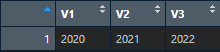
\includegraphics[width=6cm,height=1.5cm]{Images/I/I1.png}
		            \caption{Output i1}

		\end{center}
		\end{figure}
\end{frame}

\begin{frame}[fragile]
\frametitle{5.  Nhiệm vụ}
	i) \textcolor{orange}{Nhóm câu hỏi liên quan đến tổng quát dữ liệu}\\
	2) Số lượng đất nước và định danh của mỗi đất nước (hiển thị 10 đất nước đầu tiên).
		\begin{center}
			\begin{tabular}{ c l }
				iso\_code: & Country \\ 
				AFG & Afghanistan  \\ 
				OWID\_AFR & Africa \\
				ALB & Albania\\ 
				Count & Số đất nước
			\end{tabular}
		\end{center}
\end{frame}

\begin{frame}[fragile]
\frametitle{5.  Nhiệm vụ}
	i) \textcolor{orange}{Nhóm câu hỏi liên quan đến tổng quát dữ liệu}\\
	2) Số lượng đất nước và định danh của mỗi đất nước (hiển thị 10 đất nước đầu tiên).
	\begin{lstlisting}[frame=single]  
i2 <- function()
{
iso_code1 <- unique(data[,1])
location1 <- unique(data[,3])
output_i2 <- rbind(cbind
(iso_code1[1:10],location1[1:10]),
cbind("Count",length(iso_code1)))
colnames(output_i2) <- c("iso_code","location")
View(output_i2)
}
	\end{lstlisting}
\end{frame}

\begin{frame}[fragile]
\frametitle{5.  Nhiệm vụ}
	i) \textcolor{orange}{Nhóm câu hỏi liên quan đến tổng quát dữ liệu}\\
2) Số lượng đất nước và định danh của mỗi đất nước (hiển thị 10 đất nước đầu tiên).
\begin{figure}[h!]
	\begin{center}
		    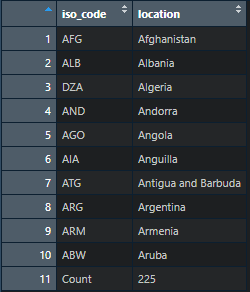
\includegraphics[scale = 0.5]{Images/I/I2.png}
		            \caption{Output i2}
		\end{center}
		\end{figure}
\end{frame}

\begin{frame}[fragile]
\frametitle{5.  Nhiệm vụ}
	i) \textcolor{orange}{Nhóm câu hỏi liên quan đến tổng quát dữ liệu}\\
	3) Số lượng châu lục trong tập mẫu
		\begin{center}
			\begin{tabular}{ c l }
				Continent : & Số châu lục \\ 
				Africa: & Châu phi \\ 
				Asia: & Châu Á \\
			\end{tabular}
		\end{center}
\end{frame}

\begin{frame}[fragile]
\frametitle{5.  Nhiệm vụ}
	i) \textcolor{orange}{Nhóm câu hỏi liên quan đến tổng quát dữ liệu}\\
	3) Số lượng châu lục trong tập mẫu
		\begin{lstlisting}[frame=single]  
i3 <- function()
{
conti <- cbind(unique(data$continent))
conti_trans <- rbind("Chau A","Chau Au",
                      "Chau Phi","Bac Mi",
                      "Nam Mi","Chau Dai Duong")
output_i3 <- data.frame(
conti,
conti_trans)
output_i3 = rbind(c
("Continent",length(conti)),output_i3)
View(output_i3)}
	\end{lstlisting}
\end{frame}

\begin{frame}[fragile]
\frametitle{5.  Nhiệm vụ}
	i) \textcolor{orange}{Nhóm câu hỏi liên quan đến tổng quát dữ liệu}\\
	3) Số lượng châu lục trong tập mẫu
\begin{figure}[h!]
	\begin{center}
		    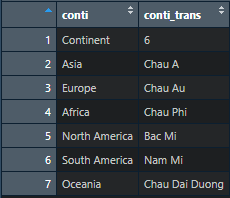
\includegraphics[scale = 0.7]{Images/I/I3.png}
		            \caption{Output i3}
		\end{center}
		\end{figure}
\end{frame}

\begin{frame}[fragile]
\frametitle{5.  Nhiệm vụ}
	i) \textcolor{orange}{Nhóm câu hỏi liên quan đến tổng quát dữ liệu}\\
	4) Số lượng dữ liệu thể hiện thu thập dữ liệu được trong từng từng châu lục và tổng số
		\begin{center}
			\begin{tabular}{ c l }
				Continent: & Observations \\ 
				Africa & value1  \\ 
				Asia & value2 \\
				Tổng: & giá trị tổng
			\end{tabular}
		\end{center}
\end{frame}

\begin{frame}[fragile]
\frametitle{5.  Nhiệm vụ}
	i) \textcolor{orange}{Nhóm câu hỏi liên quan đến tổng quát dữ liệu}\\
	4) Số lượng dữ liệu thể hiện thu thập dữ liệu được trong từng từng châu lục và tổng số
			\begin{lstlisting}[frame=single]  
i4 <- function()
{
con_data <- as.numeric(table(data$continent))
con <- sort(unique(data$continent))
sum <- c("Tong:",sum(con_data))
con_data <- data.frame(rbind(cbind(con,con_data),sum))
colnames(con_data) <- c("Continent:", "Observations")
rownames(con_data) <- c(1:nrow(con_data))
View(con_data)
}
	\end{lstlisting}
\end{frame}

\begin{frame}[fragile]
\frametitle{5.  Nhiệm vụ}
	i) \textcolor{orange}{Nhóm câu hỏi liên quan đến tổng quát dữ liệu}\\
	4) Số lượng dữ liệu thể hiện thu thập dữ liệu được trong từng từng châu lục và tổng số
\begin{figure}[h!]
	\begin{center}
		    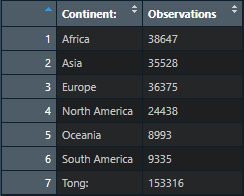
\includegraphics[scale = 0.7]{Images/I/I4.png}
		            \caption{Output i4}
		\end{center}
		\end{figure}
\end{frame}

\begin{frame}[fragile]
\frametitle{5.  Nhiệm vụ}
	i) \textcolor{orange}{Nhóm câu hỏi liên quan đến tổng quát dữ liệu}\\
	5) Số lượng dữ liệu thể hiện thu thập dữ liệu được trong từng từng đất nước (hiển thị 10 dất nước cuối cùng) và tổng số
		\begin{center}
			\begin{tabular}{ c l }
				iso\_code & Observations \\ 
				AFG & value1  \\ 
				OWID\_AFR & value2 \\
				ALB & value3\\
				Tổng: & giá trị tổng
			\end{tabular}
		\end{center}
\end{frame}

\begin{frame}[fragile]
\frametitle{5.  Nhiệm vụ}
	i) \textcolor{orange}{Nhóm câu hỏi liên quan đến tổng quát dữ liệu}\\
	5) Số lượng dữ liệu thể hiện thu thập dữ liệu được trong từng từng đất nước (hiển thị 10 dất nước cuối cùng) và tổng số
	\begin{lstlisting}[frame=single]  
con_data <- as.numeric(table(data$iso_code))
coun <- sort(unique(data$iso_code))
sum <- c("Tong:",sum(con_data))
con_data <- data.frame(rbind(cbind(coun,con_data),sum))
colnames(con_data) <- c("iso_code", "Observations")
rownames(con_data) <- c(1:nrow(con_data))
View(tail(con_data, n = 11))
	\end{lstlisting}
\end{frame}

\begin{frame}[fragile]
\frametitle{5.  Nhiệm vụ}
	i) \textcolor{orange}{Nhóm câu hỏi liên quan đến tổng quát dữ liệu}\\
	5) Số lượng dữ liệu thể hiện thu thập dữ liệu được trong từng từng đất nước (hiển thị 10 dất nước cuối cùng) và tổng số
\begin{figure}[h!]
	\begin{center}
		    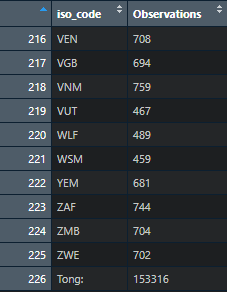
\includegraphics[scale = 0.5]{Images/I/I5.png}
		            \caption{Output i5}
		\end{center}
		\end{figure}
\end{frame}

\begin{frame}[fragile]
\frametitle{5.  Nhiệm vụ}
	i) \textcolor{orange}{Nhóm câu hỏi liên quan đến tổng quát dữ liệu}\\
	6) Cho biết các châu lục nào có lượng dữ liệu thu thập nhỏ nhất và giá trị nhó nhất đó?\\
	7) Cho biết các châu lục nào có lượng dữ liệu thu thập lớn nhất và giá trị lớn nhất đó?
\begin{figure}[h!]
	\begin{center}
		    
\includegraphics[scale = 1]{Images/I/I6.png}
		            \caption{Output i6}
		\end{center}
		\end{figure}
		\begin{figure}[h!]
	\begin{center}
		    
\includegraphics[scale = 1]{Images/I/I7.png}
		            \caption{Output i7}
		\end{center}
		\end{figure}
\end{frame}


\begin{frame}[fragile]
\frametitle{5.  Nhiệm vụ}
	i) \textcolor{orange}{Nhóm câu hỏi liên quan đến tổng quát dữ liệu}\\
	8) Cho biết các nước nào có lượng dữ liệu thu thập nhỏ nhất và giá trị nhó nhất đó?\\
	9) Cho biết các nước nào có lượng dữ liệu thu thập lớn nhất và giá trị lớn nhất đó?
		\begin{lstlisting}[frame=single]  
coun_data <- as.numeric(table(data$location))
coun <- sort(unique(data$location))
coun_data <- data.frame(cbind(coun,coun_data))
colnames(coun_data) <- c("Country", "Observations")
rownames(coun_data) <- c(1:nrow(coun_data))
coun_data[,2] <- as.numeric(coun_data[,2])
View(rbind(subset(coun_data, 
Observations == min(coun_data$Observations)),
           subset(coun_data, 
Observations == max(coun_data$Observations))))
	\end{lstlisting}
\end{frame}

\begin{frame}[fragile]
\frametitle{5.  Nhiệm vụ}
	i) \textcolor{orange}{Nhóm câu hỏi liên quan đến tổng quát dữ liệu}\\
	8) Cho biết các nước nào có lượng dữ liệu thu thập nhỏ nhất và giá trị nhó nhất đó?\\
	9) Cho biết các nước nào có lượng dữ liệu thu thập lớn nhất và giá trị lớn nhất đó?
\begin{figure}[h!]
	\begin{center}
		    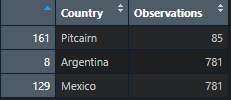
\includegraphics[scale = 1]{Images/I/I8+9.png}
		            \caption{Output i8+i9}
		\end{center}
		\end{figure}
\end{frame}

\begin{frame}[fragile]
\frametitle{5.  Nhiệm vụ}
	i) \textcolor{orange}{Nhóm câu hỏi liên quan đến tổng quát dữ liệu}\\
	10) Cho biết các date nào có lượng dữ liệu thu thập nhỏ nhất và giá trị nhó nhất đó?\\
	11) Cho biết các date nào có lượng dữ liệu thu thập lớn nhất và giá trị lớn nhất đó?
		\begin{lstlisting}[frame=single]  
coun_data <- as.numeric(table(data$location))
coun <- sort(unique(data$location))
coun_data <- data.frame(cbind(coun,coun_data))
colnames(coun_data) <- c("Country", "Observations")
rownames(coun_data) <- c(1:nrow(coun_data))
coun_data[,2] <- as.numeric(coun_data[,2])
View(rbind(subset(coun_data, 
Observations == min(coun_data$Observations)),
           subset(coun_data, 
Observations == max(coun_data$Observations))))
	\end{lstlisting}
\end{frame}

\begin{frame}[fragile]
\frametitle{5.  Nhiệm vụ}
	i) \textcolor{orange}{Nhóm câu hỏi liên quan đến tổng quát dữ liệu}\\
	10) Cho biết các date nào có lượng dữ liệu thu thập nhỏ nhất và giá trị nhó nhất đó?
\begin{figure}[h!]
	\begin{center}
		    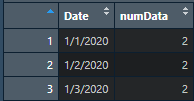
\includegraphics[scale = 1]{Images/I/I10.png}
		            \caption{Output i10}
		\end{center}
		\end{figure}
\end{frame}

\begin{frame}[fragile]
\frametitle{5.  Nhiệm vụ}
	i) \textcolor{orange}{Nhóm câu hỏi liên quan đến tổng quát dữ liệu}\\
	11) Cho biết các date nào có lượng dữ liệu thu thập lớn nhất và giá trị lớn nhất đó?
\begin{figure}[h!]
	\begin{center}
		    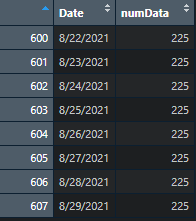
\includegraphics[scale = 0.7]{Images/I/I11.png}
		            \caption{Output i11}
		\end{center}
		\end{figure}
\end{frame}

\begin{frame}[fragile]
\frametitle{5.  Nhiệm vụ}
	i) \textcolor{orange}{Nhóm câu hỏi liên quan đến tổng quát dữ liệu}\\
		12) Cho biết số lượng dữ liệu thu thập được theo date và châu lục.\\
		13) Cho biết số lượng dữ liệu thu thập được là lớn nhất theo date và châu lục.\\
		14) Cho biết số lượng dữ liệu thu thập được là nhỏ nhất theo date và châu lục.
   \begin{lstlisting}[frame=single,basicstyle=\tiny]  
i12_i13_i14 <- function()
{
  df <- data.frame(data)
  df <- subset(df, continent != "")
  date_sort <- df %>% arrange(mdy(df$date))
  output_i12 <- date_sort %>% group_by(date, continent) 
                          %>% summarise(value = n())
  output_i12 <- output_i12 %>% arrange(mdy(output_i12$date))

  View(output_i12)

  output_i13 <- subset(output_i12, value == max(value))
  View(output_i13)

  output_i14 <- subset(output_i12, value == min(value))
  View(output_i14)
}
	\end{lstlisting}
\end{frame}

\begin{frame}[fragile]
\frametitle{5.  Nhiệm vụ}
	i) \textcolor{orange}{Nhóm câu hỏi liên quan đến tổng quát dữ liệu}\\
		12) Cho biết số lượng dữ liệu thu thập được theo date và châu lục.
\begin{figure}[h!]
	\begin{center}
		    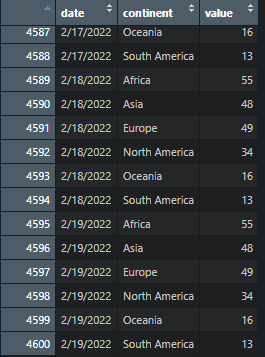
\includegraphics[scale = 0.5]{Images/I/I12.png}
		            \caption{Output i12}
		\end{center}
		\end{figure}
\end{frame}

\begin{frame}[fragile]
\frametitle{5.  Nhiệm vụ}
	i) \textcolor{orange}{Nhóm câu hỏi liên quan đến tổng quát dữ liệu}\\
	13) Cho biết số lượng dữ liệu thu thập được là lớn nhất theo date và châu lục.
	\begin{figure}[h!]
	\begin{center}
		    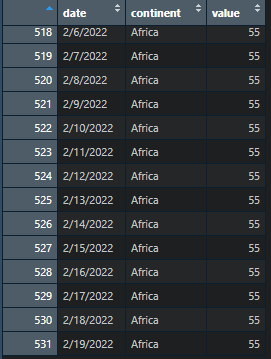
\includegraphics[scale = 0.4]{Images/I/I13.png}
		            \caption{Output i13}
		\end{center}
		\end{figure}
\end{frame}

\begin{frame}[fragile]
\frametitle{5.  Nhiệm vụ}
	i) \textcolor{orange}{Nhóm câu hỏi liên quan đến tổng quát dữ liệu}\\
	14) Cho biết số lượng dữ liệu thu thập được là nhỏ nhất theo date và châu lục.
	\begin{figure}[h!]
	\begin{center}
		    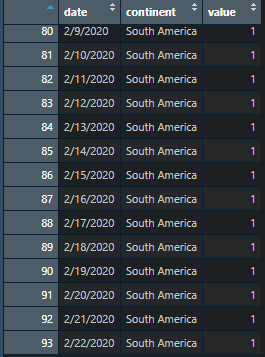
\includegraphics[scale = 0.4]{Images/I/I14.png}
		            \caption{Output i14}
		\end{center}
		\end{figure}
\end{frame}

\begin{frame}[fragile]
\frametitle{5.  Nhiệm vụ}
	i) \textcolor{orange}{Nhóm câu hỏi liên quan đến tổng quát dữ liệu}\\
	15) Với một date là k và châu lục t cho trước, hãy cho biết số lượng dữ liệu thể hiện thu thập dữ liệu được.
		\begin{lstlisting}[frame=single,basicstyle=\tiny]  
df <- data.frame(iso_code, continent,date, new_cases,death_cases)
df$date<-as.Date(df$date,format="%m/%d/%Y") 
k=readline
(prompt="Enter the k date with format %Y/%m/%d: ")
t=
readline(prompt="Enter the t continent: ")
datefilter = as.Date(k)
df <- df %>% filter(continent == t &date == datefilter)
print(df)
	\end{lstlisting}
\end{frame}

\begin{frame}[fragile]
\frametitle{5.  Nhiệm vụ}
	i) \textcolor{orange}{Nhóm câu hỏi liên quan đến tổng quát dữ liệu}\\
	15) Với một date là k và châu lục t cho trước, hãy cho biết số lượng dữ liệu thể hiện thu thập dữ liệu được.
	\begin{figure}[h!]
	\begin{center}
		    \includegraphics[scale = 0.7]{Images/I/I15.png}
		            \caption{Output i15}
		\end{center}
		\end{figure}
\end{frame}

\begin{frame}[fragile]
\frametitle{5.  Nhiệm vụ}
	i) \textcolor{orange}{Nhóm câu hỏi liên quan đến tổng quát dữ liệu}\\
	16) Có đất nước nào mà số lượng dữ liệu thu thập được là bằng nhau không? Hãy cho biết các iso\_code của đất nước đó.
		\begin{lstlisting}[frame=single]  
sub_con_data <- subset
(con_data,duplicated(con_data[,2])|
duplicated(con_data[,2],fromLast=TRUE))
sub_con_data <- 
sub_con_data[order(sub_con_data[,2]),]
View(sub_con_data)
	\end{lstlisting}
\end{frame}

\begin{frame}[fragile]
\frametitle{5.  Nhiệm vụ}
	i) \textcolor{orange}{Nhóm câu hỏi liên quan đến tổng quát dữ liệu}\\
	16) Có đất nước nào mà số lượng dữ liệu thu thập được là bằng nhau không? Hãy cho biết các iso\_code của đất nước đó.
	\begin{figure}[h!]
	\begin{center}
		    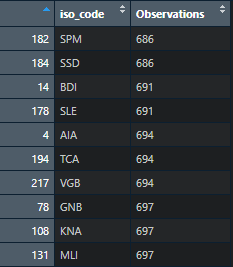
\includegraphics[scale = 1]{Images/I/I16.png}
		            \caption{Output i16}
		\end{center}
		\end{figure}
\end{frame}

\begin{frame}[fragile]
\frametitle{5.  Nhiệm vụ}
	i) \textcolor{orange}{Nhóm câu hỏi liên quan đến tổng quát dữ liệu}\\
	17) Liệt kê iso\_code, tên đất nước mà chiều dài iso\_code lớn hơn 3.
	\begin{lstlisting}[frame=single]  
i17 <- function()
{
temp <- cbind
(unique(data$iso_code),unique(data$location))
output_i17 <- temp[nchar(unique(data$iso_code))>3,]
View(output_i17)
}
	\end{lstlisting}
\end{frame}

\begin{frame}[fragile]
\frametitle{5.  Nhiệm vụ}
	i) \textcolor{orange}{Nhóm câu hỏi liên quan đến tổng quát dữ liệu}\\
	17) Liệt kê iso\_code, tên đất nước mà chiều dài iso\_code lớn hơn 3.
	\begin{figure}[h!]
	\begin{center}
		    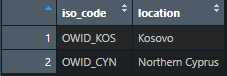
\includegraphics[scale = 1]{Images/I/I17.png}
		            \caption{Output i17}
		\end{center}
		\end{figure}
\end{frame}
\subsection{Câu ii}
\begin{frame}[fragile]
\frametitle{5.  Nhiệm vụ}
	ii) \textcolor{orange}{Nhóm câu hỏi liên quan đến mô tả thống kê cơ bản dữ liệu}\\
Với mỗi quốc gia mà thuộc về nhóm cần tính số liệu thống kê lần lượt cho nhiễm và tử vong do coronavirus được báo cáo mới:
    %%%%%%%%%ii1)%%%%%%%%%%%%%
    1) Tính giá trị nhỏ nhất, lớn nhất
    
    %%%%%%%%%%%%%ii2)%%%%%%%%%
    2) Tính tứ phân vị thứ nhất(Q1), thứ hai(Q2), thứ ba(Q3) 
    
    %%%%%%%%%%%%%ii3)%%%%%%%%%
    3) Tính giá trị trung bình (Avg)
    
    %%%%%%%%%%%%%ii4)%%%%%%%%%
    4) Tính giá trị độ lệch chuẩn (Std)
    
    %%%%%%%%%%%%%ii5)%%%%%%%%%
    5) Đếm xem có bao nhiêu outliers, một quan sát mà giá trị của nó nằm trong khoảng sau:\\
    $IQR = Q3 - Q1$\\
    $outliers < Q1 - 1.5*IQR$ hoặc $outliers > Q3 + 1.5*IQR$
    
    %%%%%%%%%%%%%ii6)%%%%%%%%%
    6) Lập bảng mô tả số liệu thống kê cho từng đất nước thuộc về nhóm: \\
\begin{center}
      \begin{tabular}{ c c c c c c c c c}
        Countries & Min & Q1 & Q2 & Q3 & Max & Avg & Std & Outlier \\ 
        ctr\_i & ? & ? & ? & ? & ? & ? & ? & ? \\ 
      \end{tabular}
    \end{center}
\end{frame}

\begin{frame}[fragile]
\frametitle{5.  Nhiệm vụ}
	ii) \textcolor{orange}{Nhóm câu hỏi liên quan đến mô tả thống kê cơ bản dữ liệu}\\
  \begin{lstlisting}[frame=single]
ii <- function(subdata, col)
{
  sum <- summary(subdata[,col])
  min <- as.numeric(sum[1])
  max <- as.numeric(sum[6])
  Q1 <- as.numeric(sum[2])
  Q2 <- as.numeric(sum[3])
  Q3 <- as.numeric(sum[5])
  avg <- as.numeric(sum[4])
  std <- sd(subdata[,col],na.rm = TRUE)
  outlier <- 0
	\end{lstlisting}
\end{frame}

\begin{frame}[fragile]
\frametitle{5.  Nhiệm vụ}
	ii) \textcolor{orange}{Nhóm câu hỏi liên quan đến mô tả thống kê cơ bản dữ liệu}\\
  \begin{lstlisting}[frame=single,basicstyle=\tiny]
  for(i in 1:nrow(subdata))
  {
    if(is.na(subdata[i,col])) next
    if(subdata[i,col] < (Q1 - (1.5*(Q3 - Q1))) || 
    subdata[i,col] > (Q3 + (1.5*(Q3 - Q1))))
    {
      outlier <- outlier + 1
    }
    else {}
  }
  return(as.numeric(c(min,Q1,Q2,Q3,max,avg,std,outlier)))
}
dfCountry <- data.frame(Countries = c("Indonesia", 
"Japan", "Vietnam"))
	\end{lstlisting}
\end{frame}

\begin{frame}[fragile]
\frametitle{5.  Nhiệm vụ}
	ii) \textcolor{orange}{Nhóm câu hỏi liên quan đến mô tả thống kê cơ bản dữ liệu}\\
\begin{lstlisting}[frame = single,basicstyle=\tiny]
id_data <- subset(data, location == "Indonesia")
jp_data <- subset(data, location == "Japan")
vn_data <- subset(data, location == "Vietnam")
tmp <- data.frame
(rbind(ii(id_data,5),ii(jp_data,5),ii(vn_data,5)))
colnames(tmp) <- c("Min", "Q1", "Q2", "Q3",
                   "Max", "Avg", "Std", "Outlier")
dfCountry_case <- cbind(dfCountry,tmp)
View(dfCountry_case)
tmp <- data.frame
(rbind(ii(id_data,6),ii(jp_data,6),ii(vn_data,6)))
colnames(tmp) <- c("Min", "Q1", "Q2", "Q3", 
                "Max", "Avg", "Std", "Outlier")
dfCountry_death <- cbind(dfCountry,tmp)
View(dfCountry_death)
	\end{lstlisting}
\end{frame}

\begin{frame}[fragile]
\frametitle{5.  Nhiệm vụ}
	ii) \textcolor{orange}{Nhóm câu hỏi liên quan đến mô tả thống kê cơ bản dữ liệu}\\
	\begin{figure}[h!]
	\begin{center}
		    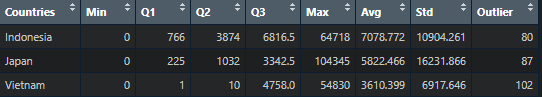
\includegraphics[scale = 0.4]{Images/II/ii1-6.png}
		            \caption{Output ii1-6: số liệu thống kê cho ca nhiễm của từng đất nước}
		\end{center}
		\end{figure}
		\begin{figure}[h!]
	\begin{center}
		    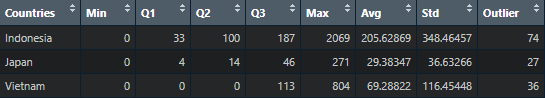
\includegraphics[scale = 0.4]{Images/II/ii1-6''.png}
		            \caption{Output ii1-6: số liệu thống kê cho tử vong của từng đất nước}
		\end{center}
		\end{figure}
\end{frame}

\begin{frame}[fragile]
\frametitle{5.  Nhiệm vụ}
	ii) \textcolor{orange}{Nhóm câu hỏi liên quan đến mô tả thống kê cơ bản dữ liệu}\\
	7) Vẽ biểu đồ boxplot hay còn được gọi là box-and-whisker cho nhiễm coronavirus
 \begin{lstlisting}[frame=single]  
boxplot(id_data[,5], jp_data[,5], vn_data[,5],
        main = "Plotbox for new cases",
        at = c(1,2,3),
        names = c("Indonesia", "Japan", "Vietnam"),
        col = c("orange","red","yellow"),
        border = "black",
        horizontal = TRUE,
        notch = TRUE
)
	\end{lstlisting}
\end{frame}

\begin{frame}[fragile]
\frametitle{5.  Nhiệm vụ}
	ii) \textcolor{orange}{Nhóm câu hỏi liên quan đến mô tả thống kê cơ bản dữ liệu}\\
	7) Vẽ biểu đồ boxplot hay còn được gọi là box-and-whisker cho nhiễm coronavirus
 \begin{lstlisting}[frame=single]  
boxplot(id_data[,6], jp_data[,6], vn_data[,6],
        main = "Plotbox for new deaths",
        at = c(1,2,3),
        names = c("Indonesia", "Japan", "Vietnam"),
        col = c("orange","red","yellow"),
        border = "black",
        horizontal = TRUE,
        notch = TRUE
)
	\end{lstlisting}
\end{frame}

\begin{frame}[fragile]
\frametitle{5.  Nhiệm vụ}
	ii) \textcolor{orange}{Nhóm câu hỏi liên quan đến mô tả thống kê cơ bản dữ liệu}\\
	7) Vẽ biểu đồ boxplot hay còn được gọi là box-and-whisker cho nhiễm coronavirus
	\begin{figure}[h!]
	\begin{center}
		    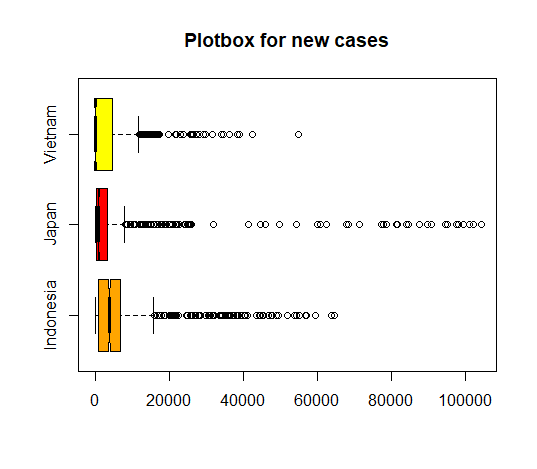
\includegraphics[scale = 0.4]{Images/II/ii7.png}
		     \caption{Output ii7}
		\end{center}
		\end{figure}
\end{frame}

\begin{frame}[fragile]
\frametitle{5.  Nhiệm vụ}
	ii) \textcolor{orange}{Nhóm câu hỏi liên quan đến mô tả thống kê cơ bản dữ liệu}\\
	7) Vẽ biểu đồ boxplot hay còn được gọi là box-and-whisker cho nhiễm coronavirus
	\begin{figure}[h!]
	\begin{center}
		    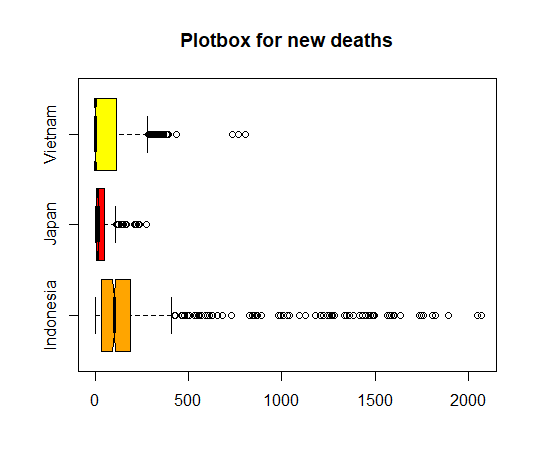
\includegraphics[scale = 0.4]{Images/II/ii7death.png}
		     \caption{Output ii7}
		\end{center}
		\end{figure}
\end{frame}

\begin{frame}[fragile]
\frametitle{5.  Nhiệm vụ}
	iii) \textcolor{orange}{Nhóm câu hỏi liên quan đến dữ liệu thể hiện thu thập dữ liệu}\\
Với mỗi quốc gia mà thuộc về nhóm cần tính số liệu thống kê lần lượt cho nhiễm và tử vong do coronavirus:
\begin{lstlisting}[frame=single]  
indo <- data[data[,1]=="IDN",]
vn <- data[data[,1]=="VNM",]
jp <- data[data[,1]=="JPN",]
	\end{lstlisting}
\end{frame}
\subsection{Câu iii}
\begin{frame}[fragile]
\frametitle{5.  Nhiệm vụ}
	iii) \textcolor{orange}{Nhóm câu hỏi liên quan đến dữ liệu thể hiện thu thập dữ liệu}\\%%%
    1) Có bao nhiêu ngày có số lần dữ liệu không được báo cáo mới
 \begin{lstlisting}[frame=single]  
nnreportcindo <- indo[is.na(indo[,5]) | indo[,5]==0,]
indo1.1 <- nrow(nnreportcindo)
view(indo1.1)
nnreportdindo <- indo[is.na(indo[,6]) | indo[,6]==0,]
indo1.2 <- nrow(nnreportdindo)
view(indo1.2)
nnreportcvn <- vn[is.na(vn[,5]) | vn[,5]==0,]
vn1.1 <- nrow(nnreportcvn)
	\end{lstlisting}
\end{frame}

\begin{frame}[fragile]
\frametitle{5.  Nhiệm vụ}
	iii) \textcolor{orange}{Nhóm câu hỏi liên quan đến dữ liệu thể hiện thu thập dữ liệu}\\%%%
    1) Có bao nhiêu ngày có số lần dữ liệu không được báo cáo mới
 \begin{lstlisting}[frame=single]  
nnreportdvn <- indo[is.na(vn[,6]) | vn[,6]==0,]
vn1.2 <- nrow(nnreportdvn)
view(vn1.1)
nnreportcjp <- jp[is.na(jp[,5]) | jp[,5]==0,]
jp1.1 <- nrow(nnreportcjp)
view(jp1.1)
nnreportdjp <- jp[is.na(jp[,6]) | jp[,6]==0,]
jp1.2 <- nrow(nnreportdjp)
view(jp1.1))
	\end{lstlisting}
\end{frame}

\begin{frame}[fragile]
\frametitle{5.  Nhiệm vụ}
	iii) \textcolor{orange}{Nhóm câu hỏi liên quan đến dữ liệu thể hiện thu thập dữ liệu}\\%%%
    1) Có bao nhiêu ngày có số lần dữ liệu không được báo cáo mới
	\begin{figure}[h!]
	\begin{center}
		    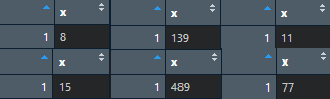
\includegraphics[scale = 1]{Images/III/iii1.png}
		     \caption{Output iii1}
		\end{center}
		\end{figure}
\end{frame}

\begin{frame}[fragile]
\frametitle{5.  Nhiệm vụ}
	iii) \textcolor{orange}{Nhóm câu hỏi liên quan đến dữ liệu thể hiện thu thập dữ liệu}\\%%%
    2) Có bao nhiêu ngày có số ca nhiễm/ tử vong là thấp nhất được báo cáo mới.
    \begin{lstlisting}[frame=single]
newreportindo<-indo[!is.na(indo[,5]) & !is.na(indo[,6]) 
                      & indo[,5]!=0 & indo[,6]!=0,]
newreportvn<-vn[!is.na(vn[,5]) & !is.na(vn[,6]) 
                  & vn[,5]!=0 & vn[,6]!=0,]
newreportjp<-jp[!is.na(jp[,5]) & !is.na(jp[,6]) 
                  & jp[,5]!=0 & jp[,6]!=0,]
newreport <- rbind
(newreportindo,newreportvn,newreportjp)
indominc <- newreportindo
[newreportindo[,5]==min(newreportindo[,5]),4]
indo2.1 <- length(indominc)
view(indo2.1)
	\end{lstlisting}
\end{frame}

\begin{frame}[fragile]
\frametitle{5.  Nhiệm vụ}
	iii) \textcolor{orange}{Nhóm câu hỏi liên quan đến dữ liệu thể hiện thu thập dữ liệu}\\%%%
    2) Có bao nhiêu ngày có số ca nhiễm/ tử vong là thấp nhất được báo cáo mới.
    \begin{lstlisting}[frame=single]  
indomind <- newreportindo
[newreportindo[,6]==min(newreportindo[,6]),4] 
indo2.2 <- length(indomind)
view(indo2.2)
vnminc <- newreportvn
[newreportvn[,5]==min(newreportvn[,5]),4] 
vn2.1 <- length(vnminc)
view(vn2.1)
vnmind <- newreportvn
[newreportvn[,6]==min(newreportvn[,6]),4] 
vn2.2 <- length(vnmind)
view(vn2.2)
	\end{lstlisting}
\end{frame}

\begin{frame}[fragile]
\frametitle{5.  Nhiệm vụ}
	iii) \textcolor{orange}{Nhóm câu hỏi liên quan đến dữ liệu thể hiện thu thập dữ liệu}\\%%%
    2) Có bao nhiêu ngày có số ca nhiễm/ tử vong là thấp nhất được báo cáo mới.
    \begin{lstlisting}[frame=single]  
jpminc <- newreportjp
[newreportjp[,5]==min(newreportjp[,5]),4] 
jp2.1 <- length(jpminc)
view(jp2.1)
jpmind <- newreportjp
[newreportjp[,6]==min(newreportjp[,6]),4] 
jp2.2 <- length(jpmind)
view(jp2.2)
	\end{lstlisting}
\end{frame}

\begin{frame}[fragile]
\frametitle{5.  Nhiệm vụ}
	iii) \textcolor{orange}{Nhóm câu hỏi liên quan đến dữ liệu thể hiện thu thập dữ liệu}\\%%%
    2) Có bao nhiêu ngày có số ca nhiễm/ tử vong là thấp nhất được báo cáo mới.
    \begin{lstlisting}[frame=single]  
jpminc <- newreportjp
[newreportjp[,5]==min(newreportjp[,5]),4] 
jp2.1 <- length(jpminc)
view(jp2.1)
jpmind <- newreportjp
[newreportjp[,6]==min(newreportjp[,6]),4] 
jp2.2 <- length(jpmind)
view(jp2.2)
	\end{lstlisting}
\end{frame}

\begin{frame}[fragile]
\frametitle{5.  Nhiệm vụ}
	iii) \textcolor{orange}{Nhóm câu hỏi liên quan đến dữ liệu thể hiện thu thập dữ liệu}\\%%%
    2) Có bao nhiêu ngày có số ca nhiễm/ tử vong là thấp nhất được báo cáo mới.
	\begin{figure}[h!]
	\begin{center}
		    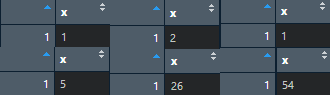
\includegraphics[scale = 1]{Images/III/iii2.png}
		     \caption{Output iii2}
		\end{center}
		\end{figure}
\end{frame}

\begin{frame}[fragile]
\frametitle{5.  Nhiệm vụ}
	iii) \textcolor{orange}{Nhóm câu hỏi liên quan đến dữ liệu thể hiện thu thập dữ liệu}\\%%%
    3) Có bao nhiêu ngày có số ca nhiễm/ tử vong là cao nhất được báo cáo mới    \begin{lstlisting}[frame=single]  
indomaxc <- newreportindo
[newreportindo[,5]==max(newreportindo[,5]),4] 
indo3.1 <- length(indomaxc)
view(indo3.1)
indomaxd <- newreportindo
[newreportindo[,6]==max(newreportindo[,6]),4] 
indo3.2 <- length(indomaxd)
view(indo3.2)
vnmaxc <- newreportvn
[newreportvn[,5]==max(newreportvn[,5]),4] 
vn3.1 <- length(vnmaxc)
view(vn3.1)
	\end{lstlisting}
\end{frame}

\begin{frame}[fragile]
\frametitle{5.  Nhiệm vụ}
	iii) \textcolor{orange}{Nhóm câu hỏi liên quan đến dữ liệu thể hiện thu thập dữ liệu}\\%%%
    3) Có bao nhiêu ngày có số ca nhiễm/ tử vong là cao nhất được báo cáo mới    \begin{lstlisting}[frame=single]  
vnmaxd <- newreportvn
[newreportvn[,6]==max(newreportvn[,6]),4] 
vn3.2 <- length(vnmaxd)
view(vn3.2)
jpmaxc <- newreportjp
[newreportjp[,5]==max(newreportjp[,5]),4] 
jp3.1 <- length(jpmaxc)
view(jp3.1)
jpmaxd <- newreportjp
[newreportjp[,6]==max(newreportjp[,6]),4] 
jp3.2 <- length(jpmaxd)
view(jp3.2)
	\end{lstlisting}
\end{frame}

\begin{frame}[fragile]
\frametitle{5.  Nhiệm vụ}
	iii) \textcolor{orange}{Nhóm câu hỏi liên quan đến dữ liệu thể hiện thu thập dữ liệu}\\%%%
    3) Có bao nhiêu ngày có số ca nhiễm/ tử vong là cao nhất được báo cáo mới 	\begin{figure}[h!]
	\begin{center}
		    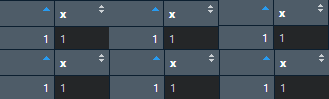
\includegraphics[scale = 1]{Images/III/iii3.png}
		     \caption{Output iii3}
		\end{center}
		\end{figure}
\end{frame}

\begin{frame}[fragile]
\frametitle{5.  Nhiệm vụ}
	iii) \textcolor{orange}{Nhóm câu hỏi liên quan đến dữ liệu thể hiện thu thập dữ liệu}\\%%%
    4) Thể hiện bảng số liệu như sau:\\
    Không được báo cáo mới:
    \begin{center}
      \begin{tabular}{ c c c }
        Countries & Infections & Deaths \\ 
        ctr\_i & value  & value\\ 
      \end{tabular}
    \end{center}
    Báo cáo mới:
    \begin{center}
      \begin{tabular}{ c c c }
        Countries & Infections & Deaths \\ 
        ctr\_i & value  & value\\ 
      \end{tabular}
    \end{center}
\end{frame}

\begin{frame}[fragile]
\frametitle{5.  Nhiệm vụ}
	iii) \textcolor{orange}{Nhóm câu hỏi liên quan đến dữ liệu thể hiện thu thập dữ liệu}\\%%%
     \begin{lstlisting}[frame=single]  
nnreport <- rbind
(indo[is.na(indo[,5]) | is.na(indo[,6]) 
| indo[,6]==0 | indo[,5]==0,],
vn[is.na(vn[,5]) | is.na(vn[,6]) 
| vn[,5]==0 | vn[,6] ==0,],
jp[is.na(jp[,5]) | is.na(jp[,6]) 
| jp[,5]==0 | jp[,6]==0,]) 
iii4.1 <- nnreport[,-c(1,2,4)]
colnames(iii4.1) <- 
c("Countries","Infections value","Deaths value")
view(iii4.1)
iii4.2 <- newreport[,-c(1,2,4)]
colnames(iii4.2) <- 
c("Countries","Infections value","Deaths value")
view(iii4.2)
	\end{lstlisting}
\end{frame}

\begin{frame}[fragile]
\frametitle{5.  Nhiệm vụ}
	iii) \textcolor{orange}{Nhóm câu hỏi liên quan đến dữ liệu thể hiện thu thập dữ liệu}\\%%%
	\begin{figure}[h!]
	\begin{center}
		    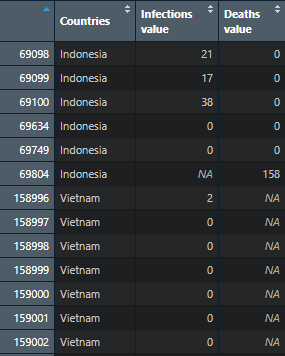
\includegraphics[scale = 0.5]{Images/III/iii4.1.png}
		     \caption{Output iii4}
		\end{center}
		\end{figure}
\end{frame}

\begin{frame}[fragile]
\frametitle{5.  Nhiệm vụ}
	iii) \textcolor{orange}{Nhóm câu hỏi liên quan đến dữ liệu thể hiện thu thập dữ liệu}\\%%%
	\begin{figure}[h!]
	\begin{center}
		    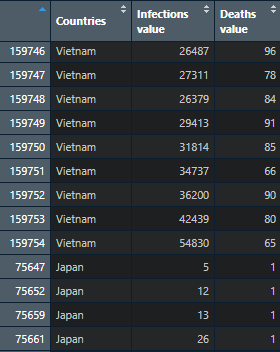
\includegraphics[scale = 0.5]{Images/III/iii4.2.png}
		     \caption{Output iii4}
		\end{center}
		\end{figure}
\end{frame}

\begin{frame}[fragile]
\frametitle{5.  Nhiệm vụ}
	iii) \textcolor{orange}{Nhóm câu hỏi liên quan đến dữ liệu thể hiện thu thập dữ liệu}\\%%%
	5) Cho biết số ngày ngắn nhất liên tiếp mà không có dữ liệu được báo cáo
     \begin{lstlisting}[frame=single]  
indo5_case <- 0
for (i in 1:nrow(indo)){
  if (is.na(indo[i,5])){
    indo5_case <- indo5_case + 1
    break}
}
view(indo5_case)
indo5_death <- 0
for (i in 1:nrow(indo)){
  if (is.na(indo[i,6])){
    indo5_death <- indo5_death + 1
    break}
}
view(indo5_death)
	\end{lstlisting}
\end{frame}

\begin{frame}[fragile]
\frametitle{5.  Nhiệm vụ}
	iii) \textcolor{orange}{Nhóm câu hỏi liên quan đến dữ liệu thể hiện thu thập dữ liệu}\\%%%
	5) Cho biết số ngày ngắn nhất liên tiếp mà không có dữ liệu được báo cáo
     \begin{lstlisting}[frame=single]  
vn5_case <- 0
for (i in 1:nrow(vn)){
  if (is.na(vn[i,5])){
    vn5_case <- vn5_case + 1
    break}
}
view(vn5_case)
vn5_death <- 0
for (i in 1:nrow(vn)){
  if (is.na(vn[i,6])){
    vn5_death <- vn5_death + 1
    break}
}
view(vn5_death)
	\end{lstlisting}
\end{frame}

\begin{frame}[fragile]
\frametitle{5.  Nhiệm vụ}
	iii) \textcolor{orange}{Nhóm câu hỏi liên quan đến dữ liệu thể hiện thu thập dữ liệu}\\%%%
	5) Cho biết số ngày ngắn nhất liên tiếp mà không có dữ liệu được báo cáo
     \begin{lstlisting}[frame=single]  
jp5_case <- 0
for (i in 1:nrow(jp)){
  if (is.na(jp[i,5])){
    jp5_case <- jp5_case + 1
    break}
}
view(jp5_case)
jp5_death <- 0
for (i in 1:nrow(jp)){
  if (is.na(jp[i,6])){
    jp5_death <- jp5_death + 1
    break}
}
view(jp5_death)
	\end{lstlisting}
\end{frame}

\begin{frame}[fragile]
\frametitle{5.  Nhiệm vụ}
	iii) \textcolor{orange}{Nhóm câu hỏi liên quan đến dữ liệu thể hiện thu thập dữ liệu}\\%%%
	\begin{figure}[h!]
	\begin{center}
		    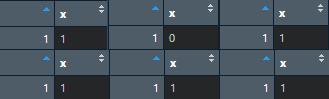
\includegraphics[scale = 1]{Images/III/iii5.png}
		     \caption{Output iii5}
		\end{center}
		\end{figure}
\end{frame}

\begin{frame}[fragile]
\frametitle{5.  Nhiệm vụ}
	iii) \textcolor{orange}{Nhóm câu hỏi liên quan đến dữ liệu thể hiện thu thập dữ liệu}\\%%%
    6) Cho biết số ngày dài nhất liên tiếp mà không có dữ liệu được báo cáo     \begin{lstlisting}[frame=single]  
indo6_case <- 0
temp <- 0
for (i in 1:nrow(indo)){
  if (is.na(indo[i,5])){
    temp <- temp + 1
    if (temp>indo6_case) {
      indo6_case <- temp
    }
  }
  else{
    temp <- 0
  }
}
view(indo6_case)
	\end{lstlisting}
\end{frame}

\begin{frame}[fragile]
\frametitle{5.  Nhiệm vụ}
	iii) \textcolor{orange}{Nhóm câu hỏi liên quan đến dữ liệu thể hiện thu thập dữ liệu}\\%%%
    6) Cho biết số ngày dài nhất liên tiếp mà không có dữ liệu được báo cáo     \begin{lstlisting}[frame=single]  
indo6_death <- 0
temp <- 0
for (i in 1:nrow(indo)){
  if (is.na(indo[i,6])){
    temp <- temp + 1
    if (temp>indo6_death) {
      indo6_death <- temp
    }
  }
  else{
    temp <- 0
  }
}
view(indo6_death)
	\end{lstlisting}
\end{frame}

\begin{frame}[fragile]
\frametitle{5.  Nhiệm vụ}
	iii) \textcolor{orange}{Nhóm câu hỏi liên quan đến dữ liệu thể hiện thu thập dữ liệu}\\%%%
    6) Cho biết số ngày dài nhất liên tiếp mà không có dữ liệu được báo cáo     \begin{lstlisting}[frame=single]  
vn6_case <- 0
temp <- 0
for (i in 1:nrow(vn)){
  if (is.na(vn[i,5])){
    temp <- temp + 1
    if (temp>vn6_case) {
      vn6_case <- temp
    }
  }
  else{
    temp <- 0
  }
}
view(vn6_case)
	\end{lstlisting}
\end{frame}

\begin{frame}[fragile]
\frametitle{5.  Nhiệm vụ}
	iii) \textcolor{orange}{Nhóm câu hỏi liên quan đến dữ liệu thể hiện thu thập dữ liệu}\\%%%
    6) Cho biết số ngày dài nhất liên tiếp mà không có dữ liệu được báo cáo     \begin{lstlisting}[frame=single]  
vn6_death <- 0
temp <- 0
for (i in 1:nrow(vn)){
  if (is.na(vn[i,6])){
    temp <- temp + 1
    if (temp>vn6_death) {
      vn6_death <- temp
    }
  }
  else{
    temp <- 0
  }
}
view(vn6_death)
	\end{lstlisting}
\end{frame}

\begin{frame}[fragile]
\frametitle{5.  Nhiệm vụ}
	iii) \textcolor{orange}{Nhóm câu hỏi liên quan đến dữ liệu thể hiện thu thập dữ liệu}\\%%%
    6) Cho biết số ngày dài nhất liên tiếp mà không có dữ liệu được báo cáo     \begin{lstlisting}[frame=single]  
jp6_case <- 0
temp <- 0
for (i in 1:nrow(jp)){
  if (is.na(jp[i,5])){
    temp <- temp + 1
    if (temp>jp6_case) {
      jp6_case <- temp
    }
  }
  else{
    temp <- 0
  }
}
view(jp6_case)
	\end{lstlisting}
\end{frame}

\begin{frame}[fragile]
\frametitle{5.  Nhiệm vụ}
	iii) \textcolor{orange}{Nhóm câu hỏi liên quan đến dữ liệu thể hiện thu thập dữ liệu}\\%%%
    6) Cho biết số ngày dài nhất liên tiếp mà không có dữ liệu được báo cáo     \begin{lstlisting}[frame=single]  
jp6_death <- 0
temp <- 0
for (i in 1:nrow(jp)){
  if (is.na(jp[i,6])){
    temp <- temp + 1
    if (temp>jp6_death) {
      jp6_death <- temp
    }
  }
  else{
    temp <- 0
  }
}
view(jp6_death)
	\end{lstlisting}
\end{frame}

\begin{frame}[fragile]
\frametitle{5.  Nhiệm vụ}
	iii) \textcolor{orange}{Nhóm câu hỏi liên quan đến dữ liệu thể hiện thu thập dữ liệu}\\%%%
    6) Cho biết số ngày dài nhất liên tiếp mà không có dữ liệu được báo cáo  
	\begin{figure}[h!]
	\begin{center}
		    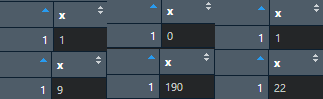
\includegraphics[scale = 1]{Images/III/iii6.png}
		     \caption{Output iii6}
		\end{center}
		\end{figure}
\end{frame}

\begin{frame}[fragile]
\frametitle{5.  Nhiệm vụ}
	iii) \textcolor{orange}{Nhóm câu hỏi liên quan đến dữ liệu thể hiện thu thập dữ liệu}\\%%%
    7) Cho biết số ngày ngắn nhất liên tiếp mà không có người nhiễm bệnh mới     \begin{lstlisting}[frame=single]  
indo7 <- 0
for (i in 1:nrow(nnreportcindo)){
  if (nnreportcindo[i,5]==0){
    indo7 <- indo7 + 1
    break}
}
view(indo7)
vn7 <- 0
for (i in 1:nrow(nnreportcvn)){
  if (nnreportcvn[i,5]==0){
    vn7 <- vn7 + 1
    break}
}
view(vn7)
jp7 <- 0
for (i in 1:nrow(nnreportcjp)){
  if (nnreportcindo[i,5]==0){
    jp7 <- jp7 + 1
    break }
}
view(jp7)
	\end{lstlisting}
\end{frame}

\begin{frame}[fragile]
\frametitle{5.  Nhiệm vụ}
	iii) \textcolor{orange}{Nhóm câu hỏi liên quan đến dữ liệu thể hiện thu thập dữ liệu}\\%%%
    7) Cho biết số ngày ngắn nhất liên tiếp mà không có người nhiễm bệnh mới
	\begin{figure}[h!]
	\begin{center}
		    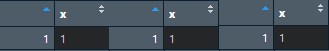
\includegraphics[scale = 1]{Images/III/iii7.png}
		     \caption{Output iii7}
		\end{center}
		\end{figure}
\end{frame}

\begin{frame}[fragile]
\frametitle{5.  Nhiệm vụ}
	iii) \textcolor{orange}{Nhóm câu hỏi liên quan đến dữ liệu thể hiện thu thập dữ liệu}\\%%%
    8) Cho biết số ngày dài nhất liên tiếp mà không có người nhiễm bệnh mới   \begin{lstlisting}[frame=single]  
indo8 <- 0
temp <- 0
for (i in 1:nrow(indo)){
  if(!is.na(indo[i,5]) & indo[i,5]==0){
    temp <- 0
  }
  else{
    temp <- temp + 1
    if (temp>indo8) {
      indo8 <- temp
    }
  }
}
view(indo8)

vn8 <- 0
temp <- 0
for (i in 1:nrow(vn)){
  if(!is.na(vn[i,5]) & vn[i,5]==0){
    temp <- 0
  }
  else{
	\end{lstlisting}
\end{frame}

\begin{frame}[fragile]
\frametitle{5.  Nhiệm vụ}
	iii) \textcolor{orange}{Nhóm câu hỏi liên quan đến dữ liệu thể hiện thu thập dữ liệu}\\%%%
    8) Cho biết số ngày dài nhất liên tiếp mà không có người nhiễm bệnh mới   \begin{lstlisting}[frame=single]  
  else{
    temp <- temp + 1
    if (temp>vn8) {
      vn8 <- temp
    }
  }
}
view(vn8)
jp8 <- 0
temp <- 0
for (i in 1:nrow(jp)){
  if(!is.na(jp[i,5]) & jp[i,5]==0){
    temp <- 0
  }
  else{
    temp <- temp + 1
    if (temp>jp8) {
      jp8 <- temp
    }
  }
}
view(jp8)
	\end{lstlisting}
\end{frame}

\begin{frame}[fragile]
\frametitle{5.  Nhiệm vụ}
	iii) \textcolor{orange}{Nhóm câu hỏi liên quan đến dữ liệu thể hiện thu thập dữ liệu}\\%%%
    8) Cho biết số ngày ngắn nhất liên tiếp mà không có người nhiễm bệnh mới
	\begin{figure}[h!]
	\begin{center}
		    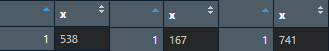
\includegraphics[scale = 1]{Images/III/iii8.png}
		     \caption{Output iii8}
		\end{center}
		\end{figure}
\end{frame}

\begin{frame}[fragile]
\frametitle{5.  Nhiệm vụ}
\subsection{Câu iv}
iv) \textcolor{red}{Nhóm câu hỏi liên quan đến trực quan dữ liệu}
    \lstset{
    title=Prep for iv1-2}
    \begin{lstlisting}[frame=single]  
freg <- data[!duplicated(data[,c('location')]),]
coun_num <- nrow(freg)
x_con <- c("Africa","Asia","Europe",
            "North America","Oceania","South America")
\end{lstlisting}
\end{frame}
\begin{frame}[fragile]
\frametitle{5.  Nhiệm vụ}
iv) \textcolor{red}{Nhóm câu hỏi liên quan đến trực quan dữ liệu}\\
   1) Vẽ biểu đồ tần số tích lũy quốc gia cho các châu lục
\begin{lstlisting}[frame=single]  
y_con <- cumsum(as.numeric(table(freg$continent)))
df_iv1 <- data.frame(Continent = x_con,Freg = y_con)
ggplot(data = df_iv1, 
aes(x = Continent, y = Freg, fill = Continent)) 
        + geom_bar(stat = "Identity", colour = "black")
\end{lstlisting}
\end{frame}

\begin{frame}[fragile]
\frametitle{5.  Nhiệm vụ}
iv) \textcolor{red}{Nhóm câu hỏi liên quan đến trực quan dữ liệu}\\
   1) Vẽ biểu đồ tần số tích lũy quốc gia cho các châu lục
	\begin{figure}[h!]
	\begin{center}
		    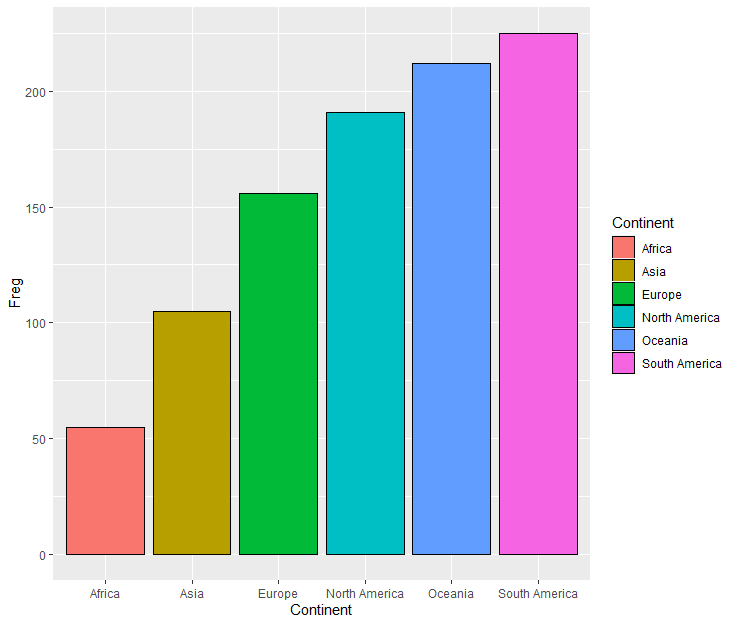
\includegraphics[scale = 0.4]{Images/IV/iv (1).png}
		     \caption{Output iv1}
		\end{center}
		\end{figure}
\end{frame}

\begin{frame}[fragile]
\frametitle{5.  Nhiệm vụ}
iv) \textcolor{red}{Nhóm câu hỏi liên quan đến trực quan dữ liệu}\\
    2) Vẽ biểu đồ tần số tương đối quốc gia cho các châu lục
\begin{lstlisting}[frame=single,basicstyle=\tiny]  
y_con <- y_con/coun_num
df_iv2 <- data.frame(Continent = x_con,Freg = y_con)
ggplot(data = df_iv2, aes(x = Continent, y = Freg, fill = Continent)) 
        + geom_bar(stat = "Identity", colour = "black")
\end{lstlisting}
\end{frame}

\begin{frame}[fragile]
\frametitle{5.  Nhiệm vụ}
	iv) \textcolor{red}{Nhóm câu hỏi liên quan đến dữ liệu thể hiện thu thập dữ liệu}\\%%%
    2) Vẽ biểu đồ tần số tương đối quốc gia cho các châu lục
	\begin{figure}[h!]
	\begin{center}
		    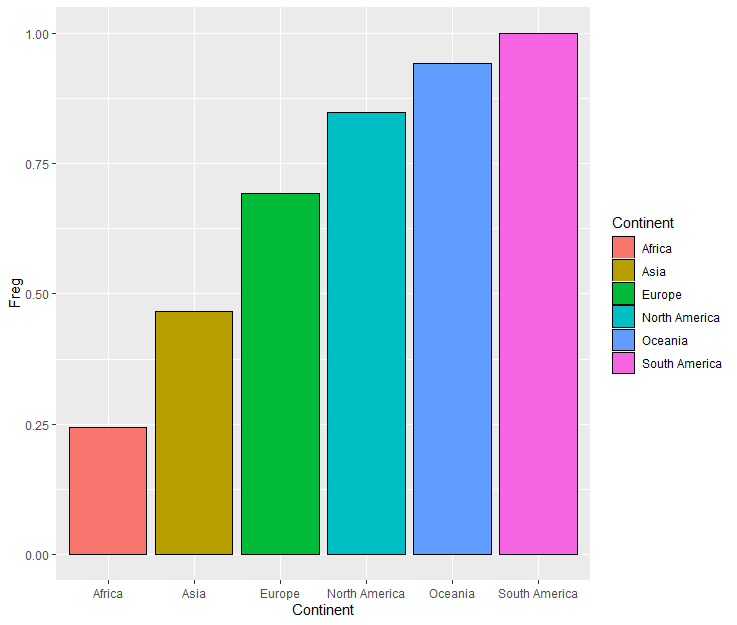
\includegraphics[scale = 0.4]{Images/IV/iv (2).png}
		     \caption{Output iv2}
		\end{center}
		\end{figure}
\end{frame}

\begin{frame}[fragile]
\frametitle{5.  Nhiệm vụ}
iv) \textcolor{red}{Nhóm câu hỏi liên quan đến trực quan dữ liệu}\\
 \lstset{
    title=Prep for iv3-4}
\begin{lstlisting}[frame=single]  
x_coun <- c("Indonesia","Japan","Vietnam")
id_data <- subset(data, location == "Indonesia")
jp_data <- subset(data, location == "Japan")
vn_data <- subset(data, location == "Vietnam")

id_date <- tail(id_data[order(as.Date(id_data$date,
                format="%d/%m/%Y")),],n=7)
jp_date <- tail(jp_data[order(as.Date(jp_data$date,
                format="%d/%m/%Y")),],n=7)
vn_date <- tail(vn_data[order(as.Date(vn_data$date,
                format="%d/%m/%Y")),],n=7)

dfDate <- data.frame(rbind(id_date,jp_date,vn_date))
\end{lstlisting}
\end{frame}

\begin{frame}[fragile]
\frametitle{5.  Nhiệm vụ}
iv) \textcolor{red}{Nhóm câu hỏi liên quan đến trực quan dữ liệu}\\
    3) Vẽ biểu đồ thể hiện nhiễm bệnh đã báo cáo của các quốc gia  mà thuộc về nhóm trong 7 ngày cuối của năm cuối cùng
\begin{lstlisting}[frame=single]  
ggplot(data = dfDate, 
aes(x = location, y = new_cases, fill = date)) 
    + geom_bar
(stat = "Identity",colour = "black",position = "dodge")
\end{lstlisting}
\end{frame}

\begin{frame}[fragile]
\frametitle{5.  Nhiệm vụ}
iv) \textcolor{red}{Nhóm câu hỏi liên quan đến trực quan dữ liệu}\\
    3) Vẽ biểu đồ thể hiện nhiễm bệnh đã báo cáo của các quốc gia  mà thuộc về nhóm trong 7 ngày cuối của năm cuối cùng
	\begin{figure}[h!]
	\begin{center}
		    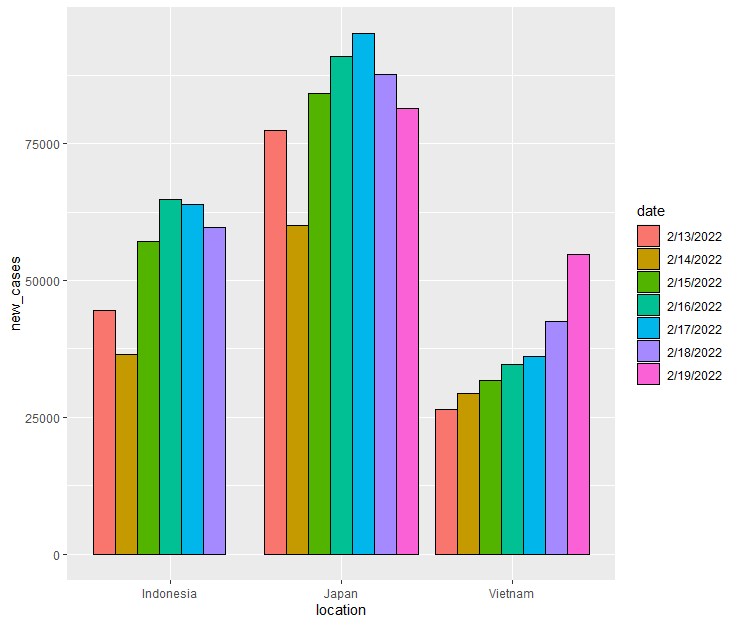
\includegraphics[scale = 0.4]{Images/IV/iv (3).png}
		     \caption{Output iv3}
		\end{center}
		\end{figure}
\end{frame}

\begin{frame}[fragile]
\frametitle{5.  Nhiệm vụ}
iv) \textcolor{red}{Nhóm câu hỏi liên quan đến trực quan dữ liệu}\\
    4) Vẽ biểu đồ thể hiện tử vong đã báo cáo của các quốc gia  mà thuộc về nhóm trong 7 ngày cuối của năm cuối cùng
\begin{lstlisting}[frame=single]  
ggplot(data = dfDate, 
aes(x = location, y = new_deaths, fill = date)) 
    + geom_bar
(stat = "Identity",colour = "black",position = "dodge")
\end{lstlisting}
\end{frame}

\begin{frame}[fragile]
\frametitle{5.  Nhiệm vụ}
	iv) \textcolor{red}{Nhóm câu hỏi liên quan đến trực quan dữ liệu}\\%%%
    4) Vẽ biểu đồ thể hiện tử vong đã báo cáo của các quốc gia  mà thuộc về nhóm trong 7 ngày cuối của năm cuối cùng
	\begin{figure}[h!]
	\begin{center}
		    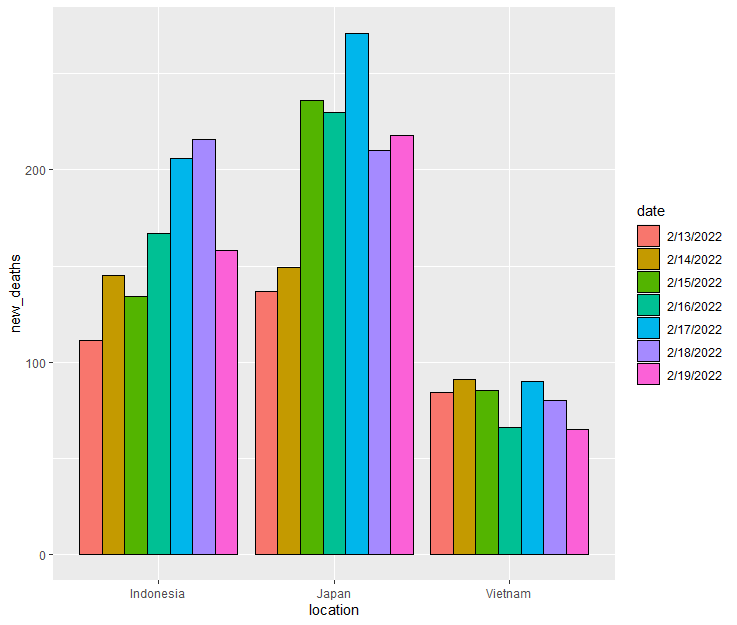
\includegraphics[scale = 0.4]{Images/IV/iv (4).png}
		     \caption{Output iv4}
		\end{center}
		\end{figure}
\end{frame}

\begin{frame}[fragile]
\frametitle{5.  Nhiệm vụ}
iv) \textcolor{red}{Nhóm câu hỏi liên quan đến trực quan dữ liệu}\\
\lstset{
    title=Function and Prep for iv5-6}
\begin{lstlisting}[frame=single]  
iv_5_6 <- function(data, name, col)
{
  subdata <- subset(data,location==name)
  sum <- summary(subdata[,col])
  Q1 <- as.numeric(sum[2])
  Q3 <- as.numeric(sum[5])
  outlier <- 0
  for(i in 1:nrow(subdata))
  {
    if(is.na(subdata[i,col])) next
    if(subdata[i,col] < (Q1 - (1.5*(Q3 - Q1))) 
       || subdata[i,col] > (Q3 + (1.5*(Q3 - Q1))))
    {
      outlier <- outlier + 1
    }
  }
  return(c(name,outlier))
}

coun_name <- unique(data[,3])
\end{lstlisting}
\end{frame}

\begin{frame}[fragile]
\frametitle{5.  Nhiệm vụ}
iv) \textcolor{red}{Nhóm câu hỏi liên quan đến trực quan dữ liệu}\\
\lstset{
    title=Function and Prep for iv5-6}
\begin{lstlisting}[frame=single]  
iv_5_6 <- function(data, name, col)
{
  subdata <- subset(data,location==name)
  sum <- summary(subdata[,col])
  Q1 <- as.numeric(sum[2])
  Q3 <- as.numeric(sum[5])
  outlier <- 0
  for(i in 1:nrow(subdata))
  {
    if(is.na(subdata[i,col])) next
    if(subdata[i,col] < (Q1 - (1.5*(Q3 - Q1))) 
       || subdata[i,col] > (Q3 + (1.5*(Q3 - Q1))))
    {
      outlier <- outlier + 1
    }
  }
  return(c(name,outlier))
}

coun_name <- unique(data[,3])
\end{lstlisting}
\end{frame}

\begin{frame}[fragile]
\frametitle{5.  Nhiệm vụ}
iv) \textcolor{red}{Nhóm câu hỏi liên quan đến trực quan dữ liệu}\\
    5) Vẽ biểu đồ phổ đất nước xuất hiện outliers cho nhiễm bệnh
\begin{lstlisting}[frame=single]  
dfOutlier <- data.frame
(Countries = c("tmp"), Outlier = c(0))
for(i in 1:length(coun_name))
{
  dfOutlier <- rbind
  (dfOutlier, iv_5_6(data,coun_name[i],5))
}
dfOutlier[,2] <- as.numeric(dfOutlier[,2])
dfOutlier <- subset(dfOutlier, Outlier != 0)
view_dfOutlier <- data.frame(rbind(subset(dfOutlier, 
                 Countries == "Indonesia"),
                 subset(dfOutlier, 
                 Countries == "Japan"),
                 subset(dfOutlier, 
                 Countries == "Vietnam")))
ggplot(data=dfOutlier, aes(x=Countries, y=Outlier))+
geom_bar(stat=Identity", colour="black")
ggplot(data = view_dfOutlier, 
      aes(x = Countries, y=Outlier, fill=Countries))+
      geom_bar(stat="Identity", colour="black")
\end{lstlisting}
\end{frame}

\begin{frame}[fragile]
\frametitle{5.  Nhiệm vụ}
	iv) \textcolor{red}{Nhóm câu hỏi liên quan đến trực quan dữ liệu}\\%%%
    5) Vẽ biểu đồ phổ đất nước xuất hiện outliers cho nhiễm bệnh
	\begin{figure}[h!]
	\begin{center}
		    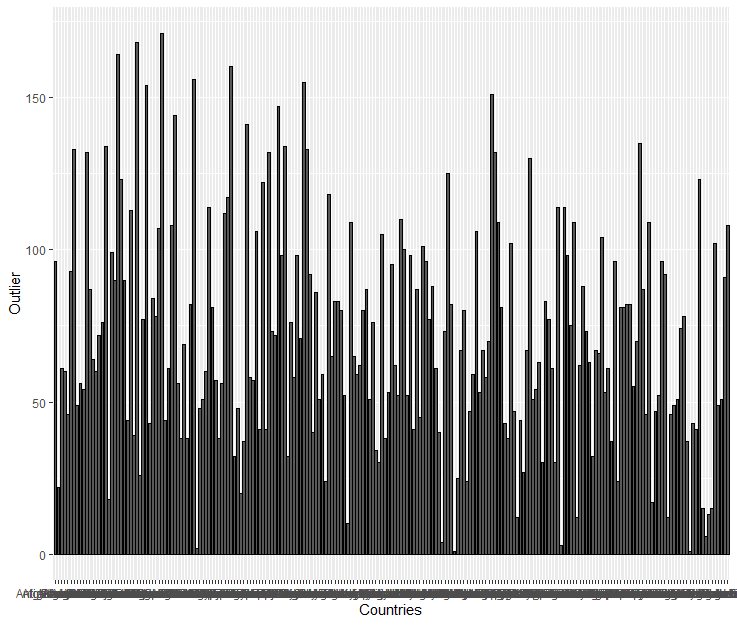
\includegraphics[scale = 0.4]{Images/IV/iv (5) - 1.png}
		     \caption{Output iv5 - 1}
		\end{center}
		\end{figure}
\end{frame}

\begin{frame}[fragile]
\frametitle{5.  Nhiệm vụ}
	iv) \textcolor{red}{Nhóm câu hỏi liên quan đến trực quan dữ liệu}\\%%%
    5) Vẽ biểu đồ phổ đất nước xuất hiện outliers cho nhiễm bệnh
	\begin{figure}[h!]
	\begin{center}
		    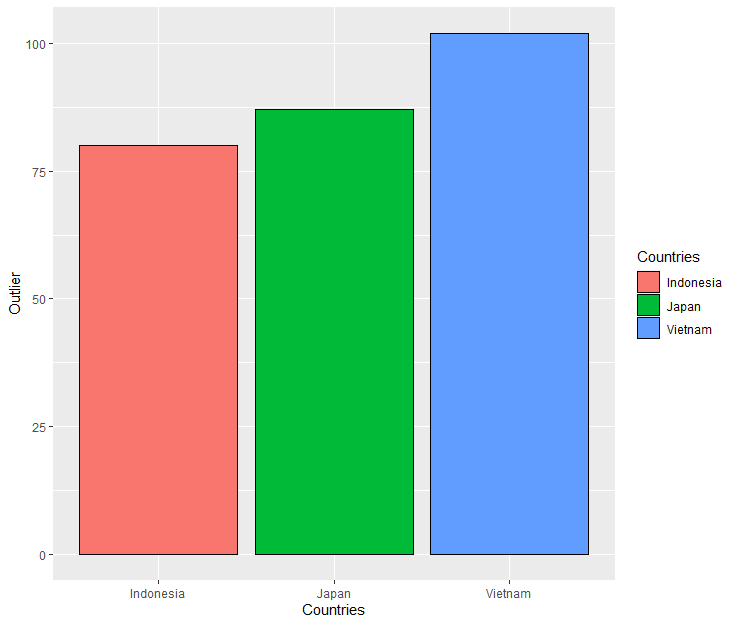
\includegraphics[scale = 0.4]{Images/IV/iv (5) - 2.png}
		     \caption{Output iv5 - 2}
		\end{center}
		\end{figure}
\end{frame}

\begin{frame}[fragile]
\frametitle{5.  Nhiệm vụ}
iv) \textcolor{red}{Nhóm câu hỏi liên quan đến trực quan dữ liệu}\\
    6) Vẽ biểu đồ phổ đất nước xuất hiện outliers cho tử vong
\begin{lstlisting}[frame=single]  
dfOutlier <- 
data.frame(Countries = c("tmp"), Outlier = c(0))
for(i in 1:length(coun_name))
{
  dfOutlier <- 
  rbind(dfOutlier, iv_5_6(data,coun_name[i],6))
}
dfOutlier[,2] <- as.numeric(dfOutlier[,2])
dfOutlier <- subset(dfOutlier, Outlier != 0)
view_dfOutlier <- data.frame(rbind(subset(dfOutlier, 
                Countries == "Indonesia"),
                subset(dfOutlier, 
                Countries == "Japan"),
                subset(dfOutlier, 
                Countries == "Vietnam")))
ggplot(data = dfOutlier, aes(x=Countries, y=Outlier))+
geom_bar(stat="Identity", colour="black")
ggplot(data=view_dfOutlier, 
aes(x=Countries, y=Outlier, 
        fill=Countries))+ 
        geom_bar(stat="Identity", colour="black")
\end{lstlisting}
\end{frame}

\begin{frame}[fragile]
\frametitle{5.  Nhiệm vụ}
	iv) \textcolor{red}{Nhóm câu hỏi liên quan đến trực quan dữ liệu}\\%%%
    6) Vẽ biểu đồ phổ đất nước xuất hiện outliers cho tử vong
	\begin{figure}[h!]
	\begin{center}
		    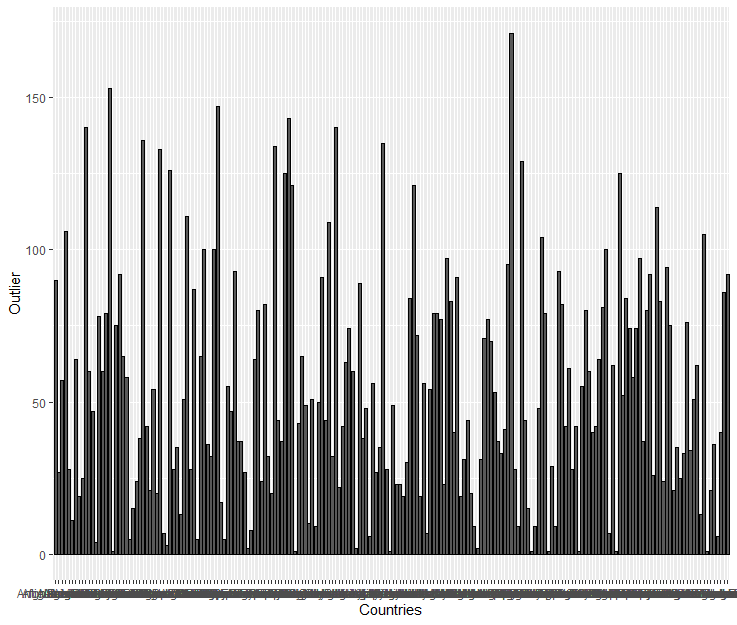
\includegraphics[scale = 0.4]{Images/IV/iv (6) - 1.png}
		     \caption{Output iv6 - 1}
		\end{center}
		\end{figure}
\end{frame}

\begin{frame}[fragile]
\frametitle{5.  Nhiệm vụ}
	iv) \textcolor{red}{Nhóm câu hỏi liên quan đến trực quan dữ liệu}\\%%%
    6) Vẽ biểu đồ phổ đất nước xuất hiện outliers cho tử vong
	\begin{figure}[h!]
	\begin{center}
		    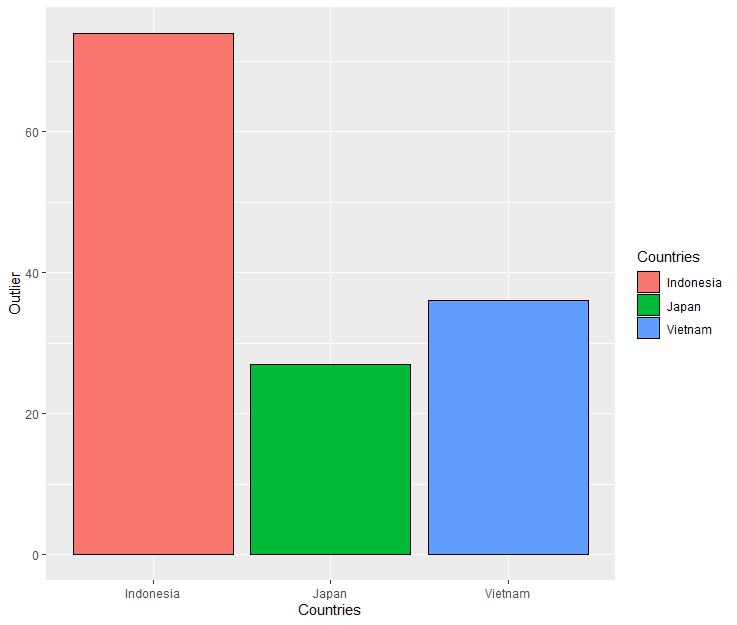
\includegraphics[scale = 0.4]{Images/IV/iv (6) - 2.png}
		     \caption{Output iv6 - 2}
		\end{center}
		\end{figure}
\end{frame}

\begin{frame}[fragile]
\frametitle{5.  Nhiệm vụ}
\lstset{
    title=Function and data for v vi vii viii}
\begin{lstlisting}[frame = single,basicstyle=\tiny]
data2 <- data
[data[,3]%in%c("Vietnam","Japan","Indonesia"),]
data2 <- rbind(data2,world_data)
data2[,4] <- as.POSIXct(data2[,4], format = "%m/%d/%Y")
y2020 <- data2[format(data2[,4],format="%Y")=="2020"& 
(format(data2[,4],format="%m")=="02" | 
format(data2[,4],format="%m")=="01" | 
format(data2[,4],format="%m")=="07" | 
format(data2[,4],format="%m")=="09"),]
y2021 <- data2[format(data2[,4],format="%Y")=="2021"& 
(format(data2[,4],format="%m")=="02" | 
format(data2[,4],format="%m")=="01" | 
format(data2[,4],format="%m")=="07" | 
format(data2[,4],format="%m")=="09"),]
y2022 <- data2[format(data2[,4],format="%Y")=="2022"& 
(format(data2[,4],format="%m")=="02" | 
format(data2[,4],format="%m")=="01" | 
format(data2[,4],format="%m")=="07" | 
format(data2[,4],format="%m")=="09"),]
y2022 <- data2[format(data2[,4],format="%Y")=="2022"& 
(format(data2[,4],format="%m")=="02" | 
format(data2[,4],format="%m")=="01" | 
format(data2[,4],format="%m")=="07" | 
format(data2[,4],format="%m")=="09"),]
\end{lstlisting}
\end{frame}

\begin{frame}[fragile]
\frametitle{5.  Nhiệm vụ}
\lstset{
    title=Function and data for v vi vii viii}
\begin{lstlisting}[frame = single,basicstyle=\tiny]
y2020_1 <- data2[format(data2[,4],format="%Y")=="2020"& 
            (format(data2[,4],format="%m")=="11" | 
             format(data2[,4],format="%m")=="12"),]

y2021_1 <- data2[format(data2[,4],format="%Y")=="2021"& 
            (format(data2[,4],format="%m")=="11" | 
            format(data2[,4],format="%m")=="12"),]

y2022_1 <- data2[format(data2[,4],format="%Y")=="2022"& 
            (format(data2[,4],format="%m")=="11" | 
            format(data2[,4],format="%m")=="12"),]
\end{lstlisting}
\end{frame}

\begin{frame}[fragile]
\frametitle{5.  Nhiệm vụ}
\lstset{
    title=Function and data for v vi vii viii}
\begin{lstlisting}[frame = single,basicstyle=\tiny]
draw_chart <- function(year_data, month_data, yyyy,cases_or_deaths,avg_or_not="")
{
  if(dim(year_data) == 0)
  return(ggplot()+labs(x="",y=paste(cases_or_deaths,"",yyyy))+
  theme(legend.position="top")+ggtitle("NA"))
  amedumb <- 5
  pain <- "Cases"
  if(cases_or_deaths == "deaths"){
    pain <- "Deaths"
    amedumb <- 6 }
  if(avg_or_not == "avg")
  {
    tmp <- ave_handle(year_data, month_data, amedumb)
    year_data[,amedumb] <- tmp
  }
  chart_out <- ggplot(data=year_data, aes(x=format(year_data[,4],format="%d"),
  y=year_data[,amedumb],color=month_data,group=month_data))+
    geom_line(lwd=1)+
    labs(x="",y=paste(pain,"",yyyy))+
    theme(legend.position="top")
  return(chart_out)
}

\end{lstlisting}
\end{frame}

\begin{frame}[fragile]
\frametitle{5.  Nhiệm vụ}
\lstset{
    title=Function and data for v vi vii viii}
\begin{lstlisting}[frame = single,basicstyle=\tiny]
cum_rel <- function(year_data, month_data, yyyy, 
 cases_or_deaths,avg_or_not=""){
  if(dim(year_data) == 0)
  return(ggplot()+
  labs(x="",y=paste(cases_or_deaths,"",yyyy))+
  theme(legend.position="top")+ggtitle("NA"))
  amedumb <- 5
  pain <- "Cases"
  if(cases_or_deaths == "deaths"){
    pain <- "Deaths"
    amedumb <- 6   }
  if(avg_or_not == "avg"){
    tmp <- ave_handle(year_data,month_data,amedumb)
    year_data[,amedumb] <- tmp}
  cum_sum_data <- cbind(cumsum(year_data[,amedumb]))
  prob <- cum_sum_data/sum(year_data[,amedumb])
  year_data[,amedumb] <- prob      
  chart_out <- ggplot(data=year_data,aes(x=year_data[,4],y=ear_data[,amedumb],group=1))+
    geom_line(lwd=1)+
    labs(x="Dates",y=paste(pain,"_crf",yyyy))+
scale_x_datetime(date_labels = "%m/%d/%Y",date_breaks = "1 week")+
    theme(legend.position="top")
  return(chart_out)}
\end{lstlisting}
\end{frame}

\begin{frame}[fragile]
\frametitle{5.  Nhiệm vụ}
\lstset{
    title=Function and data for v vi vii viii}
\begin{lstlisting}[frame = single,basicstyle=\tiny]
cum <- function(year_data,
month_data,yyyy,cases_or_deaths,avg_or_not="")
{
  if(dim(year_data) == 0) return(ggplot()+
  labs(x="",y=paste(cases_or_deaths,"",yyyy))+
  theme(legend.position="top")+ggtitle("NA"))
  amedumb <- 5
  pain <- "Cases"
  if(cases_or_deaths == "deaths"){
    pain <- "Deaths"
    amedumb <- 6 
  }
  if(avg_or_not == "avg")
  {
    tmp <- ave_handle(year_data, month_data, amedumb)
    year_data[,amedumb] <- tmp
  }
  cum_sum_data <- cbind(cumsum(year_data[,amedumb]))
  prob <- cum_sum_data
  year_data[,amedumb] <- prob
  chart_out <- ggplot(data=year_data,aes(x=format(year_data[,4],format="%d"),
  y=year_data[,amedumb],
  color=month_data,group=month_data))+geom_line(lwd=1)+
    labs(x="",y=paste("Cumulavite of",pain,"",yyyy))+
    theme(legend.position="top")
  return(chart_out)}
\end{lstlisting}
\end{frame}

\begin{frame}[fragile]
\frametitle{5.  Nhiệm vụ}
\begin{lstlisting}[frame = single,basicstyle=\tiny]

two_line_chart <- function(year_data, month_data, yyyy,
cases_or_deaths,avg_or_not="")
{
  if(dim(year_data) == 0) 
  return(ggplot()+labs(x="",y=paste("Cases and Deaths","",yyyy))+
  theme(legend.position="top")+ggtitle("NA"))
  cases <- c()
  deaths <- c()
  mon_uni <- cbind(month_data)
  if(avg_or_not == "avg")
  {
  tmp <- ave_handle(year_data, month_data, 5)
  year_data[,5] <- tmp
  tmp <- ave_handle(year_data, month_data, 6)
  year_data[,6] <- tmp
  }
\end{lstlisting}
\end{frame}

\begin{frame}[fragile]
\frametitle{5.  Nhiệm vụ}
\begin{lstlisting}[frame = single,basicstyle=\tiny]
for(x in 1:length(mon_uni))
  {
    cases <- rbind(cases,paste("New_cases",toString(mon_uni[x])))
    deaths <- rbind(deaths,paste("New_deaths",toString(mon_uni[x])))
  }
  cases_and_deaths <- rbind(cases,deaths)
  chart_out <- ggplot(data=year_data,
  aes(x=format(year_data[,4],format="%d"),group=month_data))+
    geom_line(lwd=1, aes(y = year_data[,5], colour = cases))+
    geom_line(lwd=1, aes(y = year_data[,6], colour = deaths))+
    labs(x="",y=paste("Cases and Deaths","",yyyy))+
    theme(legend.position="top")
  return(chart_out)
}
\end{lstlisting}
\end{frame}

\begin{frame}[fragile]
\frametitle{5.  Nhiệm vụ}
\begin{lstlisting}[frame = single,basicstyle=\tiny]
ave_7days <- function(mon)
{
  i <- 1
  j <- 1
  arr <- cbind(mon)
  arr[is.na(arr)] <- 0
  wah <- arr
  lenlen <- length(arr)
  while(i < lenlen + 1)
  {
    wah[i] <- arr[j:i]/(i - j + 1)
    if(i >= 7)
    {
      j <- j + 1
    }
    i <- i + 1
  }
  while(j < i)
  {
    wah[j] <- arr[j:i]/(i - j + 1)
    #print(i - j + 1)
    j <- j + 1
  }
  return(wah)
}
\end{lstlisting}
\end{frame}

\begin{frame}[fragile]
\frametitle{5.  Nhiệm vụ}
\begin{lstlisting}[frame = single,basicstyle=\tiny]
ave_handle <- function(df, mon, amedumb)
{
  mon_uni <- cbind(unique(mon))
  df[is.na(df)] <- 0
  arr <- c()
  for(x in mon_uni)
  {
    tmp <- df[format(df[,4],format="%m")==x,]
    arr <- rbind(arr,ave_7days(tmp[,amedumb]))
  }
  return(arr)
}

country_chart <- function(country, type_w, made, cases_or_deaths = "", 
chart_name, avg_or_not = "")
{
\end{lstlisting}
\end{frame}

\begin{frame}[fragile]
\frametitle{5.  Nhiệm vụ}
\begin{lstlisting}[frame = single,basicstyle=\tiny]
Months_2020<-format(y2020[y2020[,3]==country,4],format="%m")
  Months_2021<-format(y2021[y2021[,3]==country,4],format="%m")
  Months_2022<-format(y2022[y2022[,3]==country,4],format="%m")
  
  Last_months_2020<-format(y2020_1[y2020_1[,3]==country,4],format="%m")
  Last_months_2021<-format(y2021_1[y2021_1[,3]==country,4],format="%m")
  Last_months_2022<-format(y2022_1[y2022_1[,3]==country,4],format="%m")
  if(type_w == "line_chart")
  {
    if(made == "2_1_7_9")
    {
      chart_2020 <- draw_chart(y2020[y2020[,3] == country,], 
      Months_2020, "2020", cases_or_deaths,avg_or_not)
      chart_2021 <- draw_chart(y2021[y2021[,3] == country,], 
      Months_2021, "2021", cases_or_deaths,avg_or_not)
      chart_2022 <- draw_chart(y2022[y2022[,3] == country,], 
      Months_2022, "2022", cases_or_deaths,avg_or_not)
      ggsave(filename = paste(chart_name,country,".jpeg"), 
      plot = arrangeGrob(chart_2020, chart_2021, chart_2022), 
      device = "jpeg", scale = 1, width = 9, height = 9)
    }
\end{lstlisting}
\end{frame}

\begin{frame}[fragile]
\frametitle{5.  Nhiệm vụ}
\begin{lstlisting}[frame = single,basicstyle=\tiny]
 else
    {
      chart_2020 <- draw_chart(y2020_1[y2020_1[,3] == country,],
      Last_months_2020, "2020", cases_or_deaths,avg_or_not)
      chart_2021 <- draw_chart(y2021_1[y2021_1[,3] == country,],
      Last_months_2021, "2021", cases_or_deaths,avg_or_not)
      chart_2022 <- draw_chart(y2022_1[y2022_1[,3] == country,],
      Last_months_2022, "2022", cases_or_deaths,avg_or_not)
      ggsave(filename = paste(chart_name,country,".jpeg"), 
      plot = arrangeGrob(chart_2020, chart_2021, chart_2022), 
      device = "jpeg", scale = 1, width = 9, height = 9)
    }
  }
  else if(type_w == "two_line")
  {
    if(made == "2_1_7_9")
    {
      chart_2020 <- two_line_chart(y2020[y2020[,3] == country,], 
      Months_2020, "2020", cases_or_deaths,avg_or_not)
      chart_2021 <- two_line_chart(y2021[y2021[,3] == country,], 
      Months_2021, "2021", cases_or_deaths,avg_or_not)
      chart_2022 <- two_line_chart(y2022[y2022[,3] == country,], 
      Months_2022, "2022", cases_or_deaths,avg_or_not)
      ggsave(filename = paste(chart_name,country,".jpeg"), 
      plot = arrangeGrob(chart_2020, chart_2021, chart_2022), 
      device = "jpeg", scale = 1, width = 9, height = 9)
    }
\end{lstlisting}
\end{frame}

\begin{frame}[fragile]
\frametitle{5.  Nhiệm vụ}
\begin{lstlisting}[frame = single,basicstyle=\tiny]
 else
    {
      chart_2020 <- two_line_chart(y2020_1[y2020_1[,3] == country,],
      Last_months_2020, "2020", cases_or_deaths,avg_or_not)
      chart_2021 <- two_line_chart(y2021_1[y2021_1[,3] == country,],
      Last_months_2021, "2021", cases_or_deaths,avg_or_not)
      chart_2022 <- two_line_chart(y2022_1[y2022_1[,3] == country,],
      Last_months_2022, "2022", cases_or_deaths,avg_or_not)
      ggsave(filename = paste(chart_name,country,".jpeg"), 
      plot = arrangeGrob(chart_2020, chart_2021, chart_2022), 
      device = "jpeg", scale = 1, width = 9, height = 9)
    }
  }
  else if(type_w == "cum") 
  {
    if(made == "2_1_7_9")
    {
      chart_2020 <- cum(y2020[y2020[,3] == country,],
      Months_2020, "2020", cases_or_deaths,avg_or_not)
      chart_2021 <- cum(y2021[y2021[,3] == country,], 
      Months_2021, "2021", cases_or_deaths,avg_or_not)
      chart_2022 <- cum(y2022[y2022[,3] == country,], 
      Months_2022, "2022", cases_or_deaths,avg_or_not)
      ggsave(filename = paste(chart_name,country,".jpeg"), 
      plot = arrangeGrob(chart_2020, chart_2021, chart_2022), 
      device = "jpeg", scale = 1, width = 9, height = 9)
    }
\end{lstlisting}
\end{frame}

\begin{frame}[fragile]
\frametitle{5.  Nhiệm vụ}
\begin{lstlisting}[frame = single,basicstyle=\tiny]
 else if(made == "11_12")
    {
      chart_2020 <- cum(y2020_1[y2020_1[,3] == country,], 
      Last_months_2020, "2020", cases_or_deaths,avg_or_not)
      chart_2021 <- cum(y2021_1[y2021_1[,3] == country,], 
      Last_months_2021, "2021", cases_or_deaths,avg_or_not)
      chart_2022 <- cum(y2022_1[y2022_1[,3] == country,], 
      Last_months_2022, "2022", cases_or_deaths,avg_or_not)
      ggsave(filename = paste(chart_name,country,".jpeg"), 
      plot = arrangeGrob(chart_2020, chart_2021, chart_2022), 
      device = "jpeg", scale = 1, width = 9, height = 9)
    }
  }
  else 
  {
    if(made == "2_1_7_9")
    {
      chart_2020 <- cum_rel(y2020[y2020[,3] == country,], 
      Months_2020, "2020", cases_or_deaths,avg_or_not)
      chart_2021 <- cum_rel(y2021[y2021[,3] == country,],
      Months_2021, "2021", cases_or_deaths,avg_or_not)
      chart_2022 <- cum_rel(y2022[y2022[,3] == country,], 
      Months_2022, "2022", cases_or_deaths,avg_or_not)
      ggsave(filename = paste(chart_name,country,".jpeg"), 
      plot = arrangeGrob(chart_2020, chart_2021, chart_2022), 
      device = "jpeg", scale = 1, width = 9, height = 9)
    }
\end{lstlisting}
\end{frame}

\begin{frame}[fragile]
\frametitle{5.  Nhiệm vụ}
\begin{lstlisting}[frame = single,basicstyle=\tiny]
  else if(made == "11_12")
    {
      chart_2020 <- cum_rel(y2020_1[y2020_1[,3] == country,], 
      Last_months_2020, "2020", cases_or_deaths,avg_or_not)
      chart_2021 <- cum_rel(y2021_1[y2021_1[,3] == country,], 
      Last_months_2021, "2021", cases_or_deaths,avg_or_not)
      chart_2022 <- cum_rel(y2022_1[y2022_1[,3] == country,], 
      Last_months_2022, "2022", cases_or_deaths,avg_or_not)
      ggsave(filename = paste(chart_name,country,".jpeg"), 
      plot = arrangeGrob(chart_2020, chart_2021, chart_2022), 
      device = "jpeg", scale = 1, width = 9, height = 9)
    }
  }
}
\end{lstlisting}
\end{frame}
\subsection{Câu v}
\begin{frame}[fragile]
\frametitle{5.  Nhiệm vụ}
v) \textcolor{red}{Nhóm câu hỏi liên quan đến trực quan dữ liệu theo thời gian là tháng}\\
Với mỗi quốc gia mà thuộc về nhóm, trên từng năm hãy vẽ biểu đồ thể hiện trục Ox là thời gian, trục Oy là nhiễm bệnh/tử vong. Hãy dùng 4 ký số của mã đề để vẽ 4 tháng tương ứng theo ký số đó. Nếu ký số là 0 thì lấy tháng là 10\\
    1) Biểu đồ thể hiện thu thập dữ liệu nhiễm bệnh cho từng tháng
    	\begin{lstlisting}[frame=single,basicstyle=\tiny]  
country_chart("Vietnam","line_chart","2_1_7_9","cases","v1")
country_chart("Japan","line_chart","2_1_7_9","cases","v1")
country_chart("Indonesia","line_chart","2_1_7_9","cases","v1")
		\end{lstlisting}
\end{frame}

\begin{frame}[fragile]
\frametitle{5.  Nhiệm vụ}
v) \textcolor{red}{Nhóm câu hỏi liên quan đến trực quan dữ liệu theo thời gian là tháng}\\
    1) Biểu đồ thể hiện thu thập dữ liệu nhiễm bệnh cho từng tháng
	\begin{figure}[h!]
	\begin{center}
		    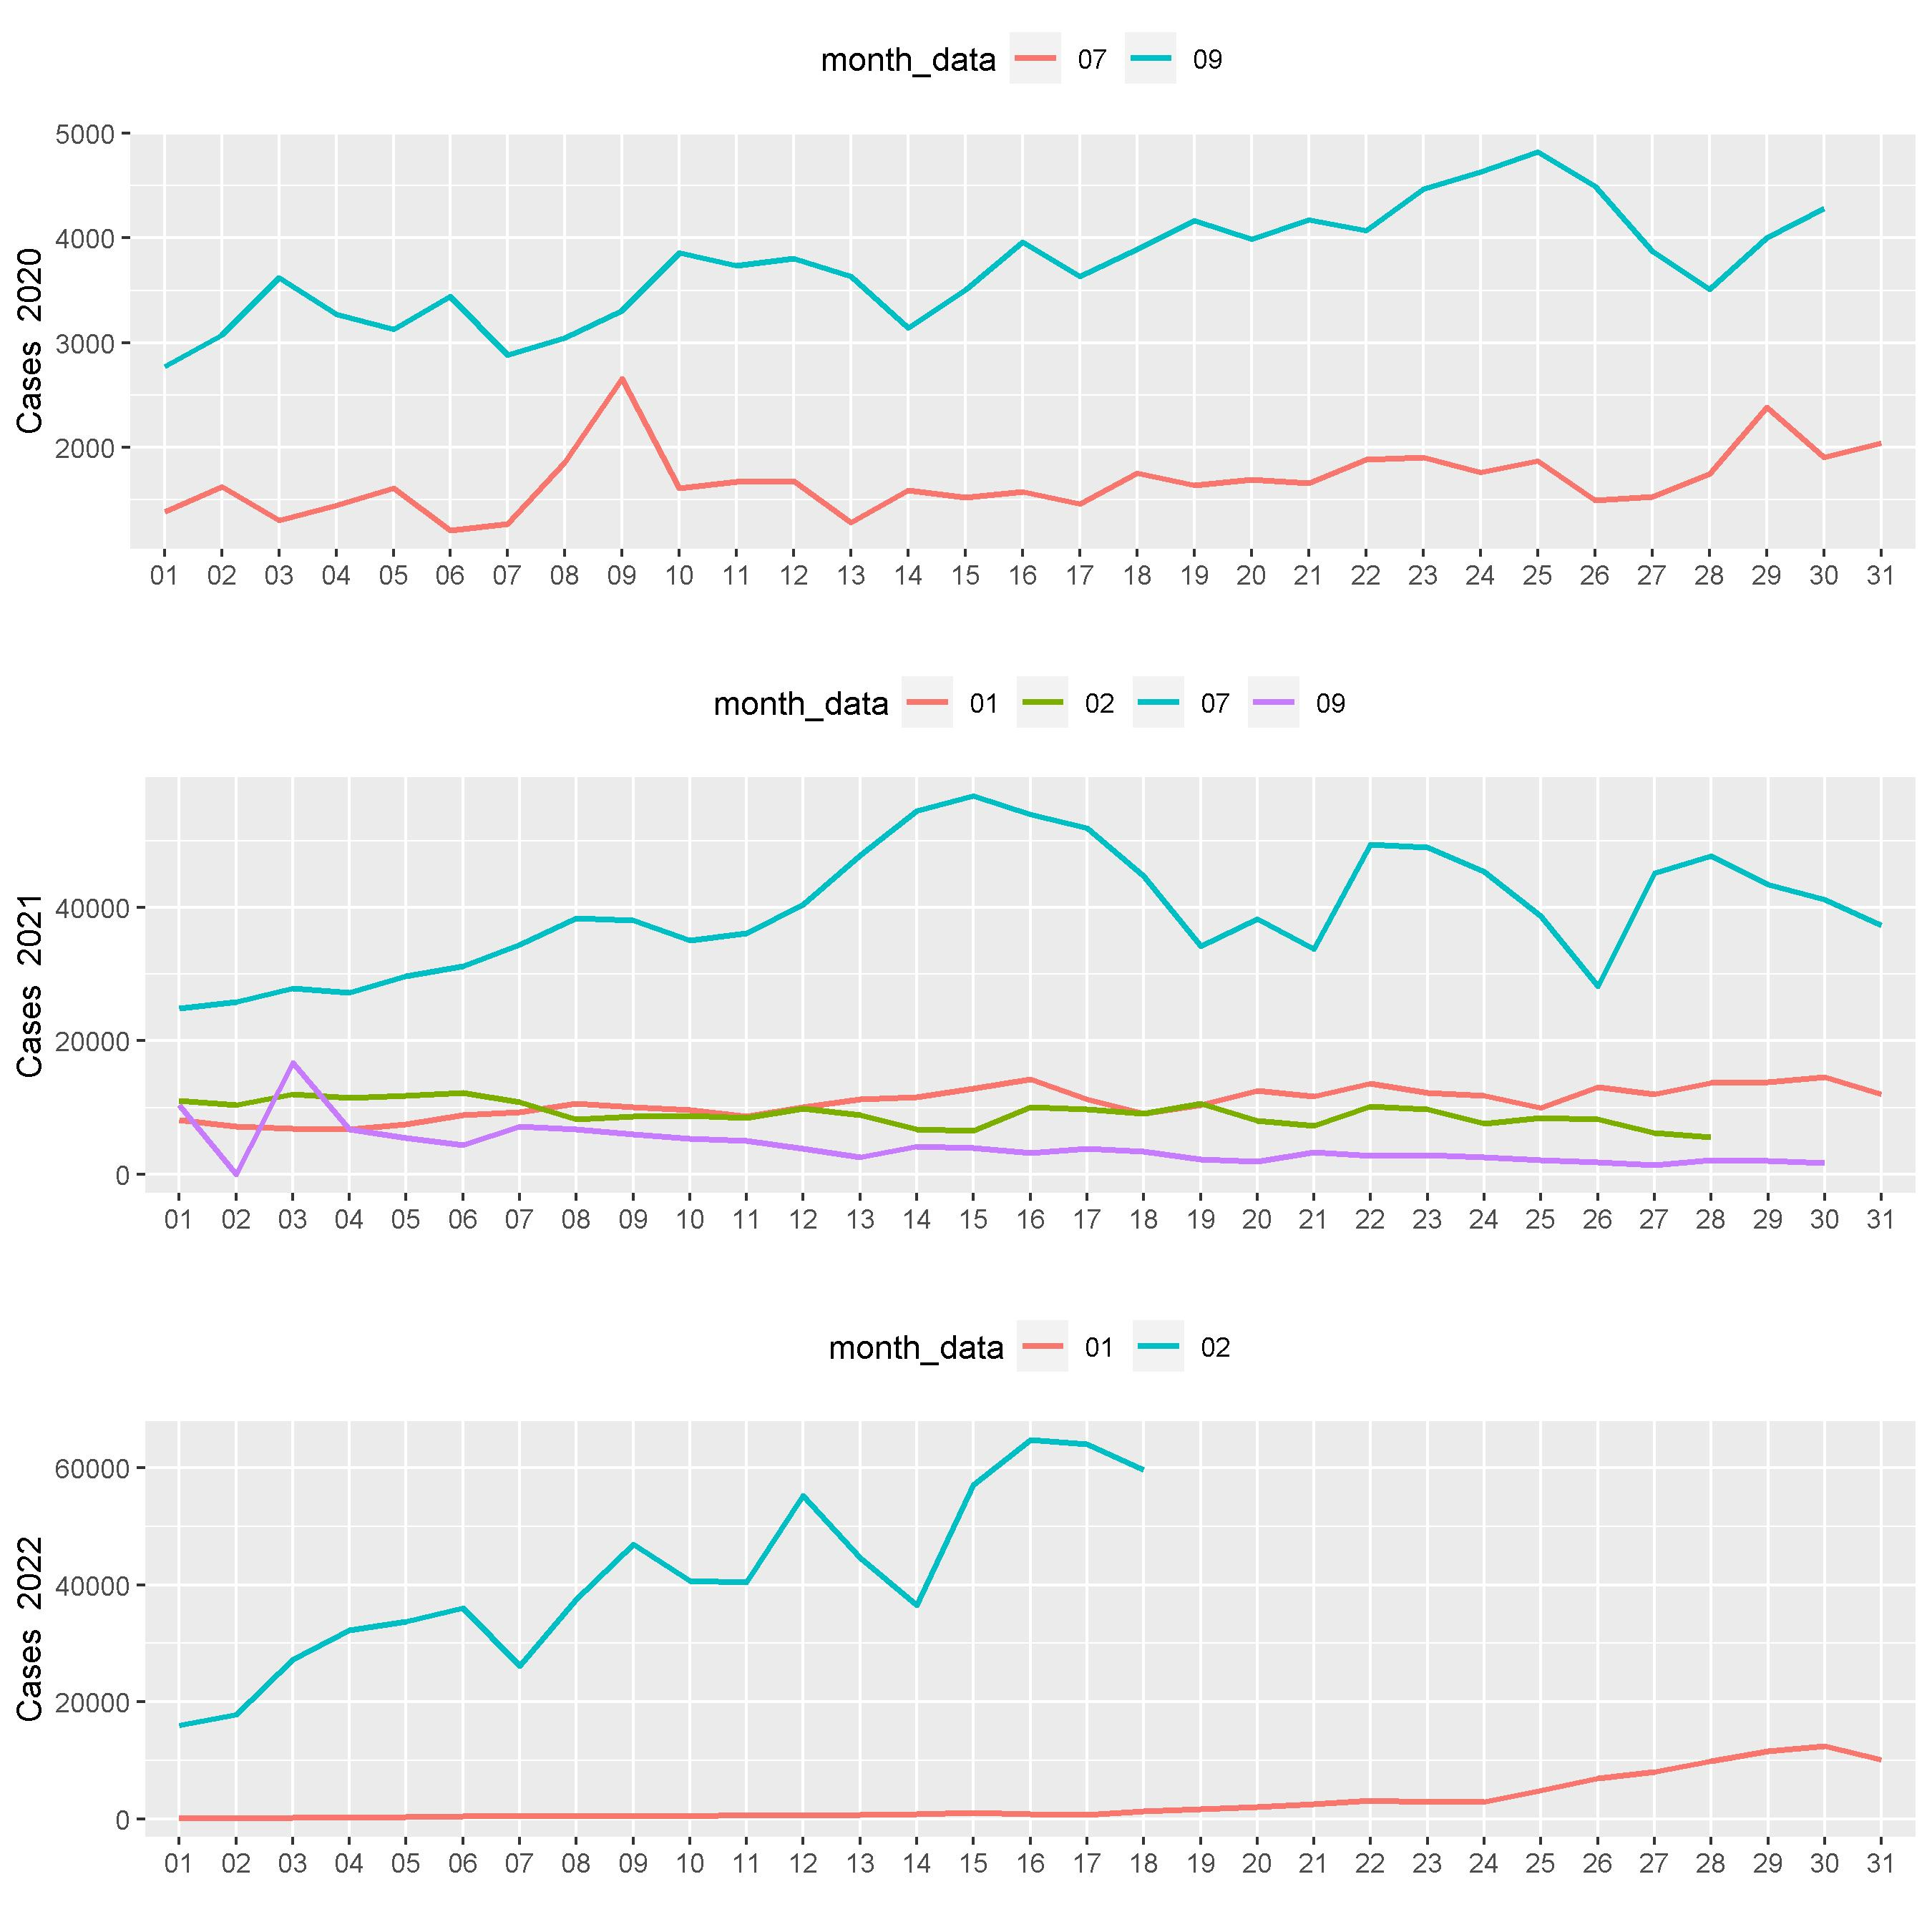
\includegraphics[scale = 0.28]{Images/V/v1 Indonesia .jpeg}
		     \caption{Output v1: Biểu đồ thể hiện thu thập dữ liệu nhiễm bệnh của Indonesia}
		\end{center}
		\end{figure}
\end{frame}

\begin{frame}[fragile]
\frametitle{5.  Nhiệm vụ}
v) \textcolor{red}{Nhóm câu hỏi liên quan đến trực quan dữ liệu theo thời gian là tháng}\\
    1) Biểu đồ thể hiện thu thập dữ liệu nhiễm bệnh cho từng tháng
	\begin{figure}[h!]
	\begin{center}
		    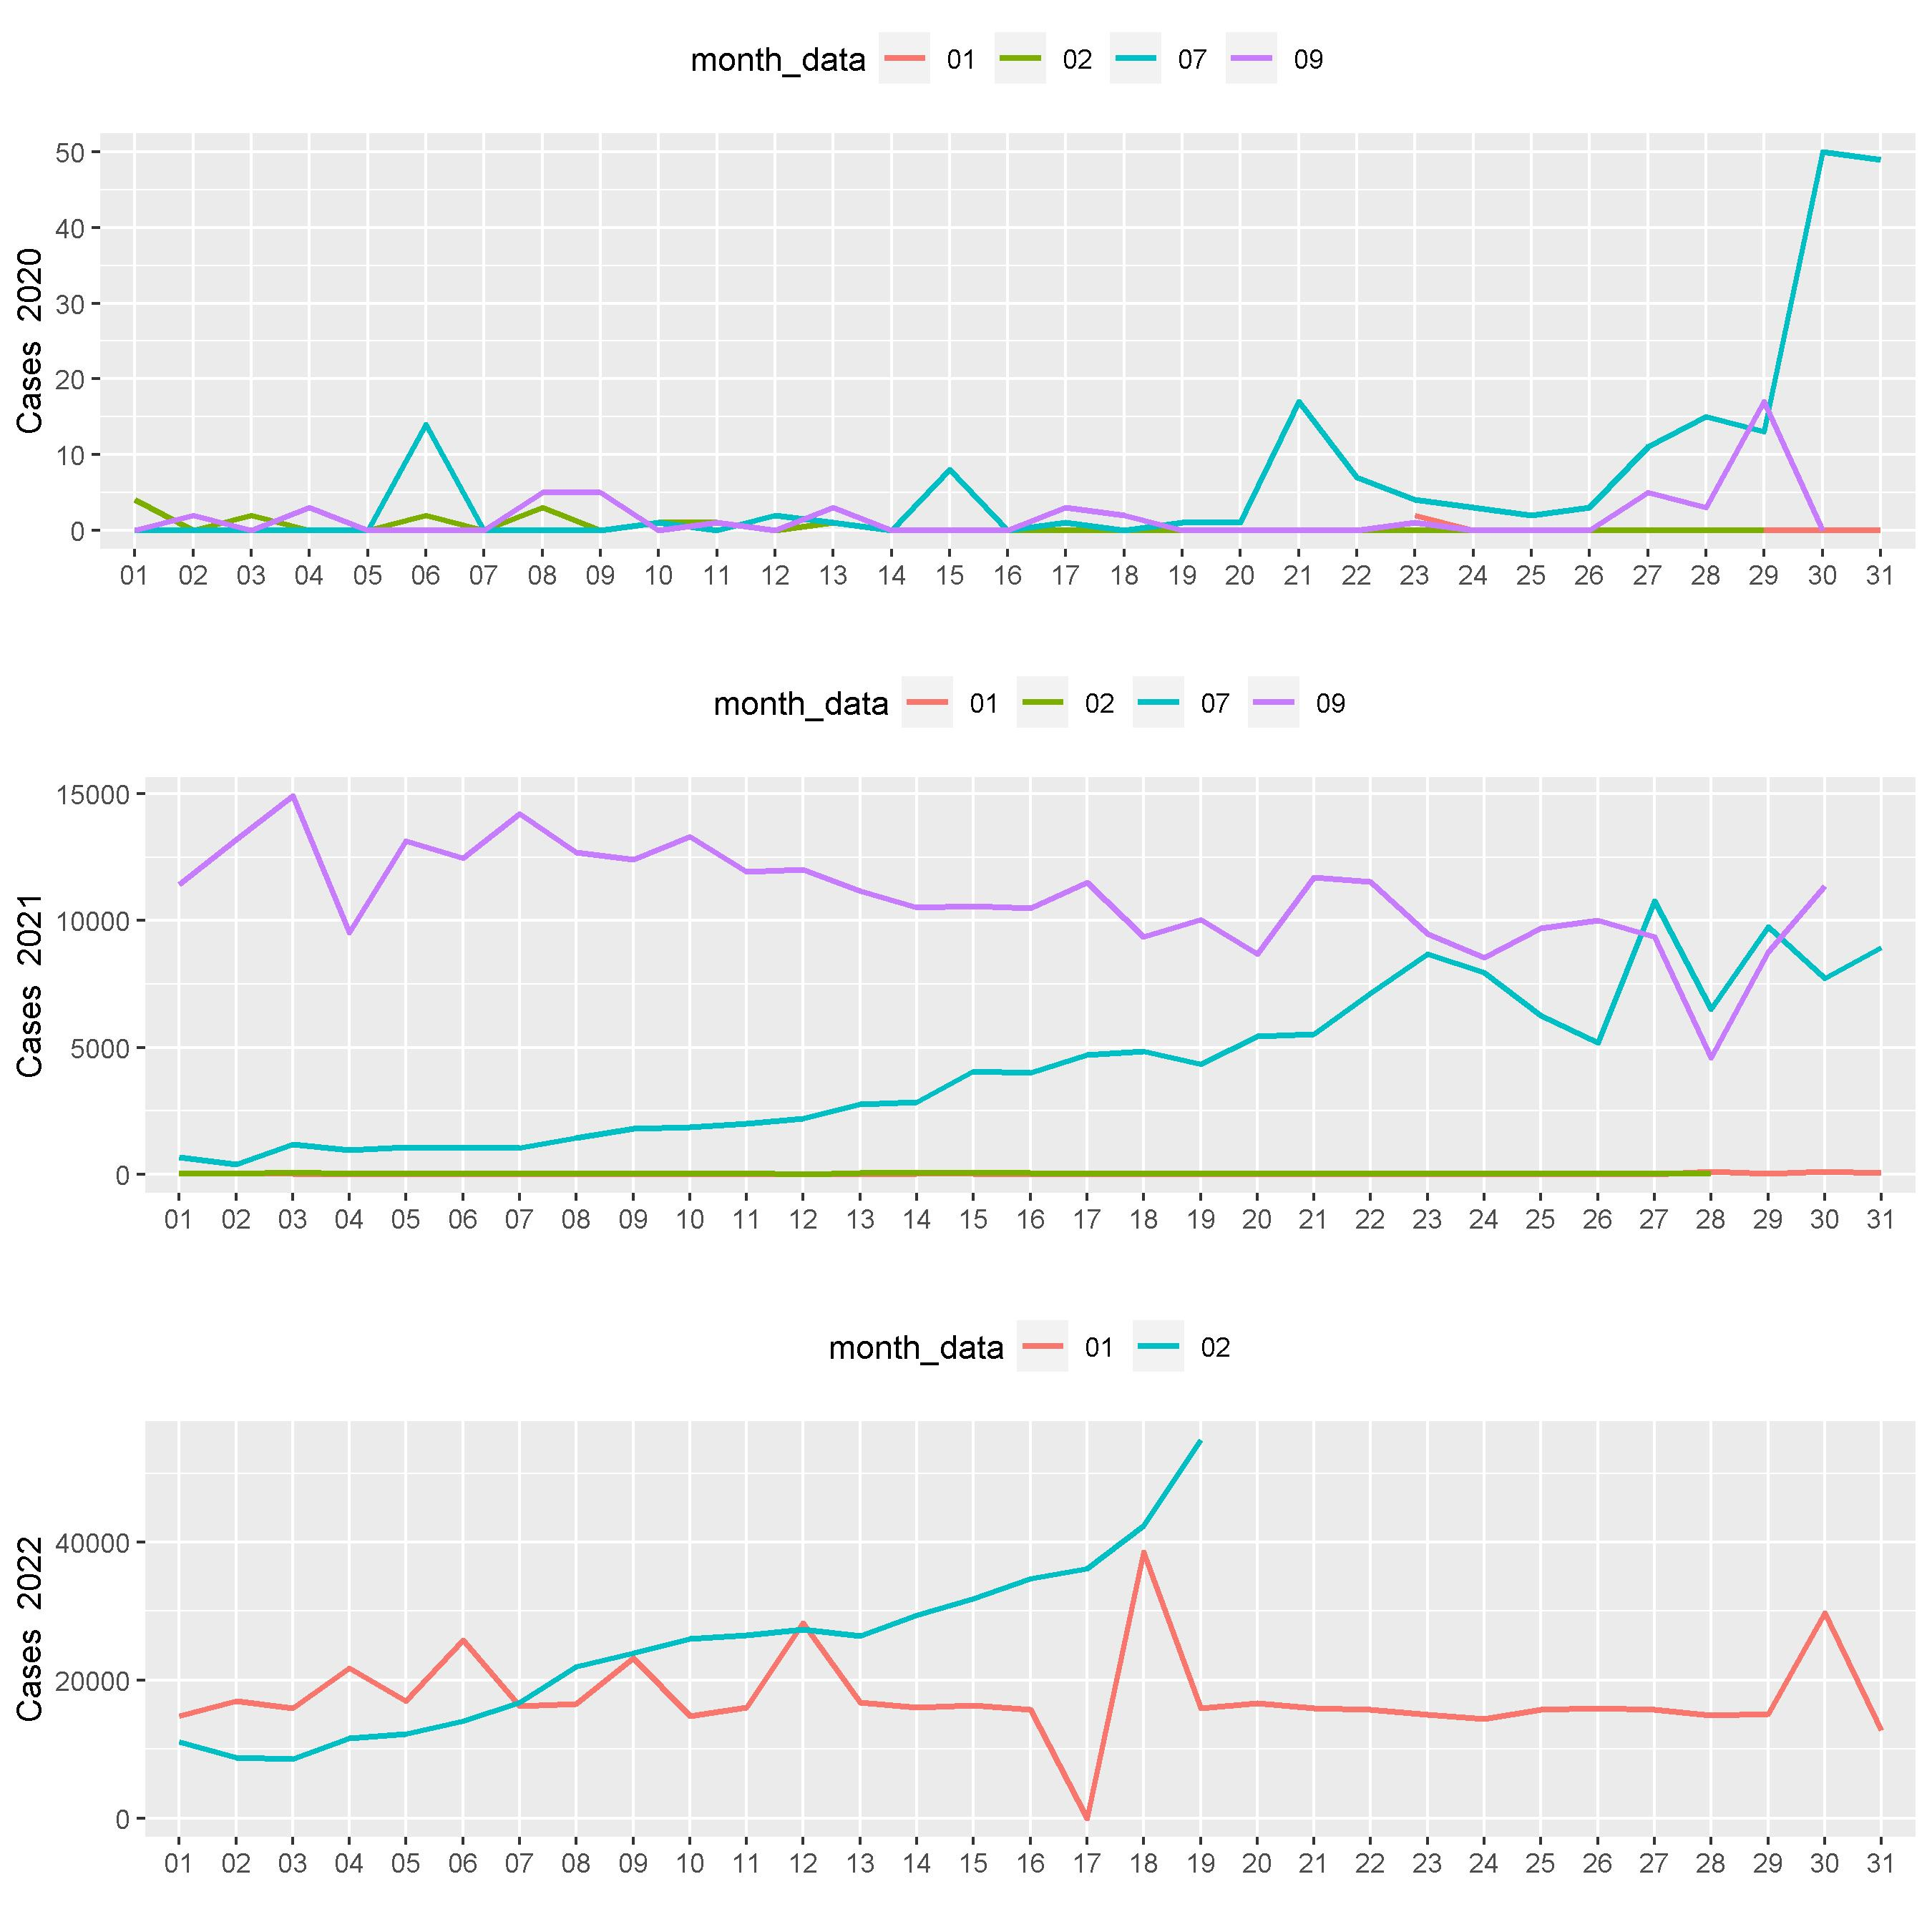
\includegraphics[scale = 0.28]{Images/V/v1 Vietnam .jpeg}
		     \caption{Output v1: Biểu đồ thể hiện thu thập dữ liệu nhiễm bệnh của Việt Nam}
		\end{center}
		\end{figure}
\end{frame}

\begin{frame}[fragile]
\frametitle{5.  Nhiệm vụ}
v) \textcolor{red}{Nhóm câu hỏi liên quan đến trực quan dữ liệu theo thời gian là tháng}\\
    1) Biểu đồ thể hiện thu thập dữ liệu nhiễm bệnh cho từng tháng
	\begin{figure}[h!]
	\begin{center}
		    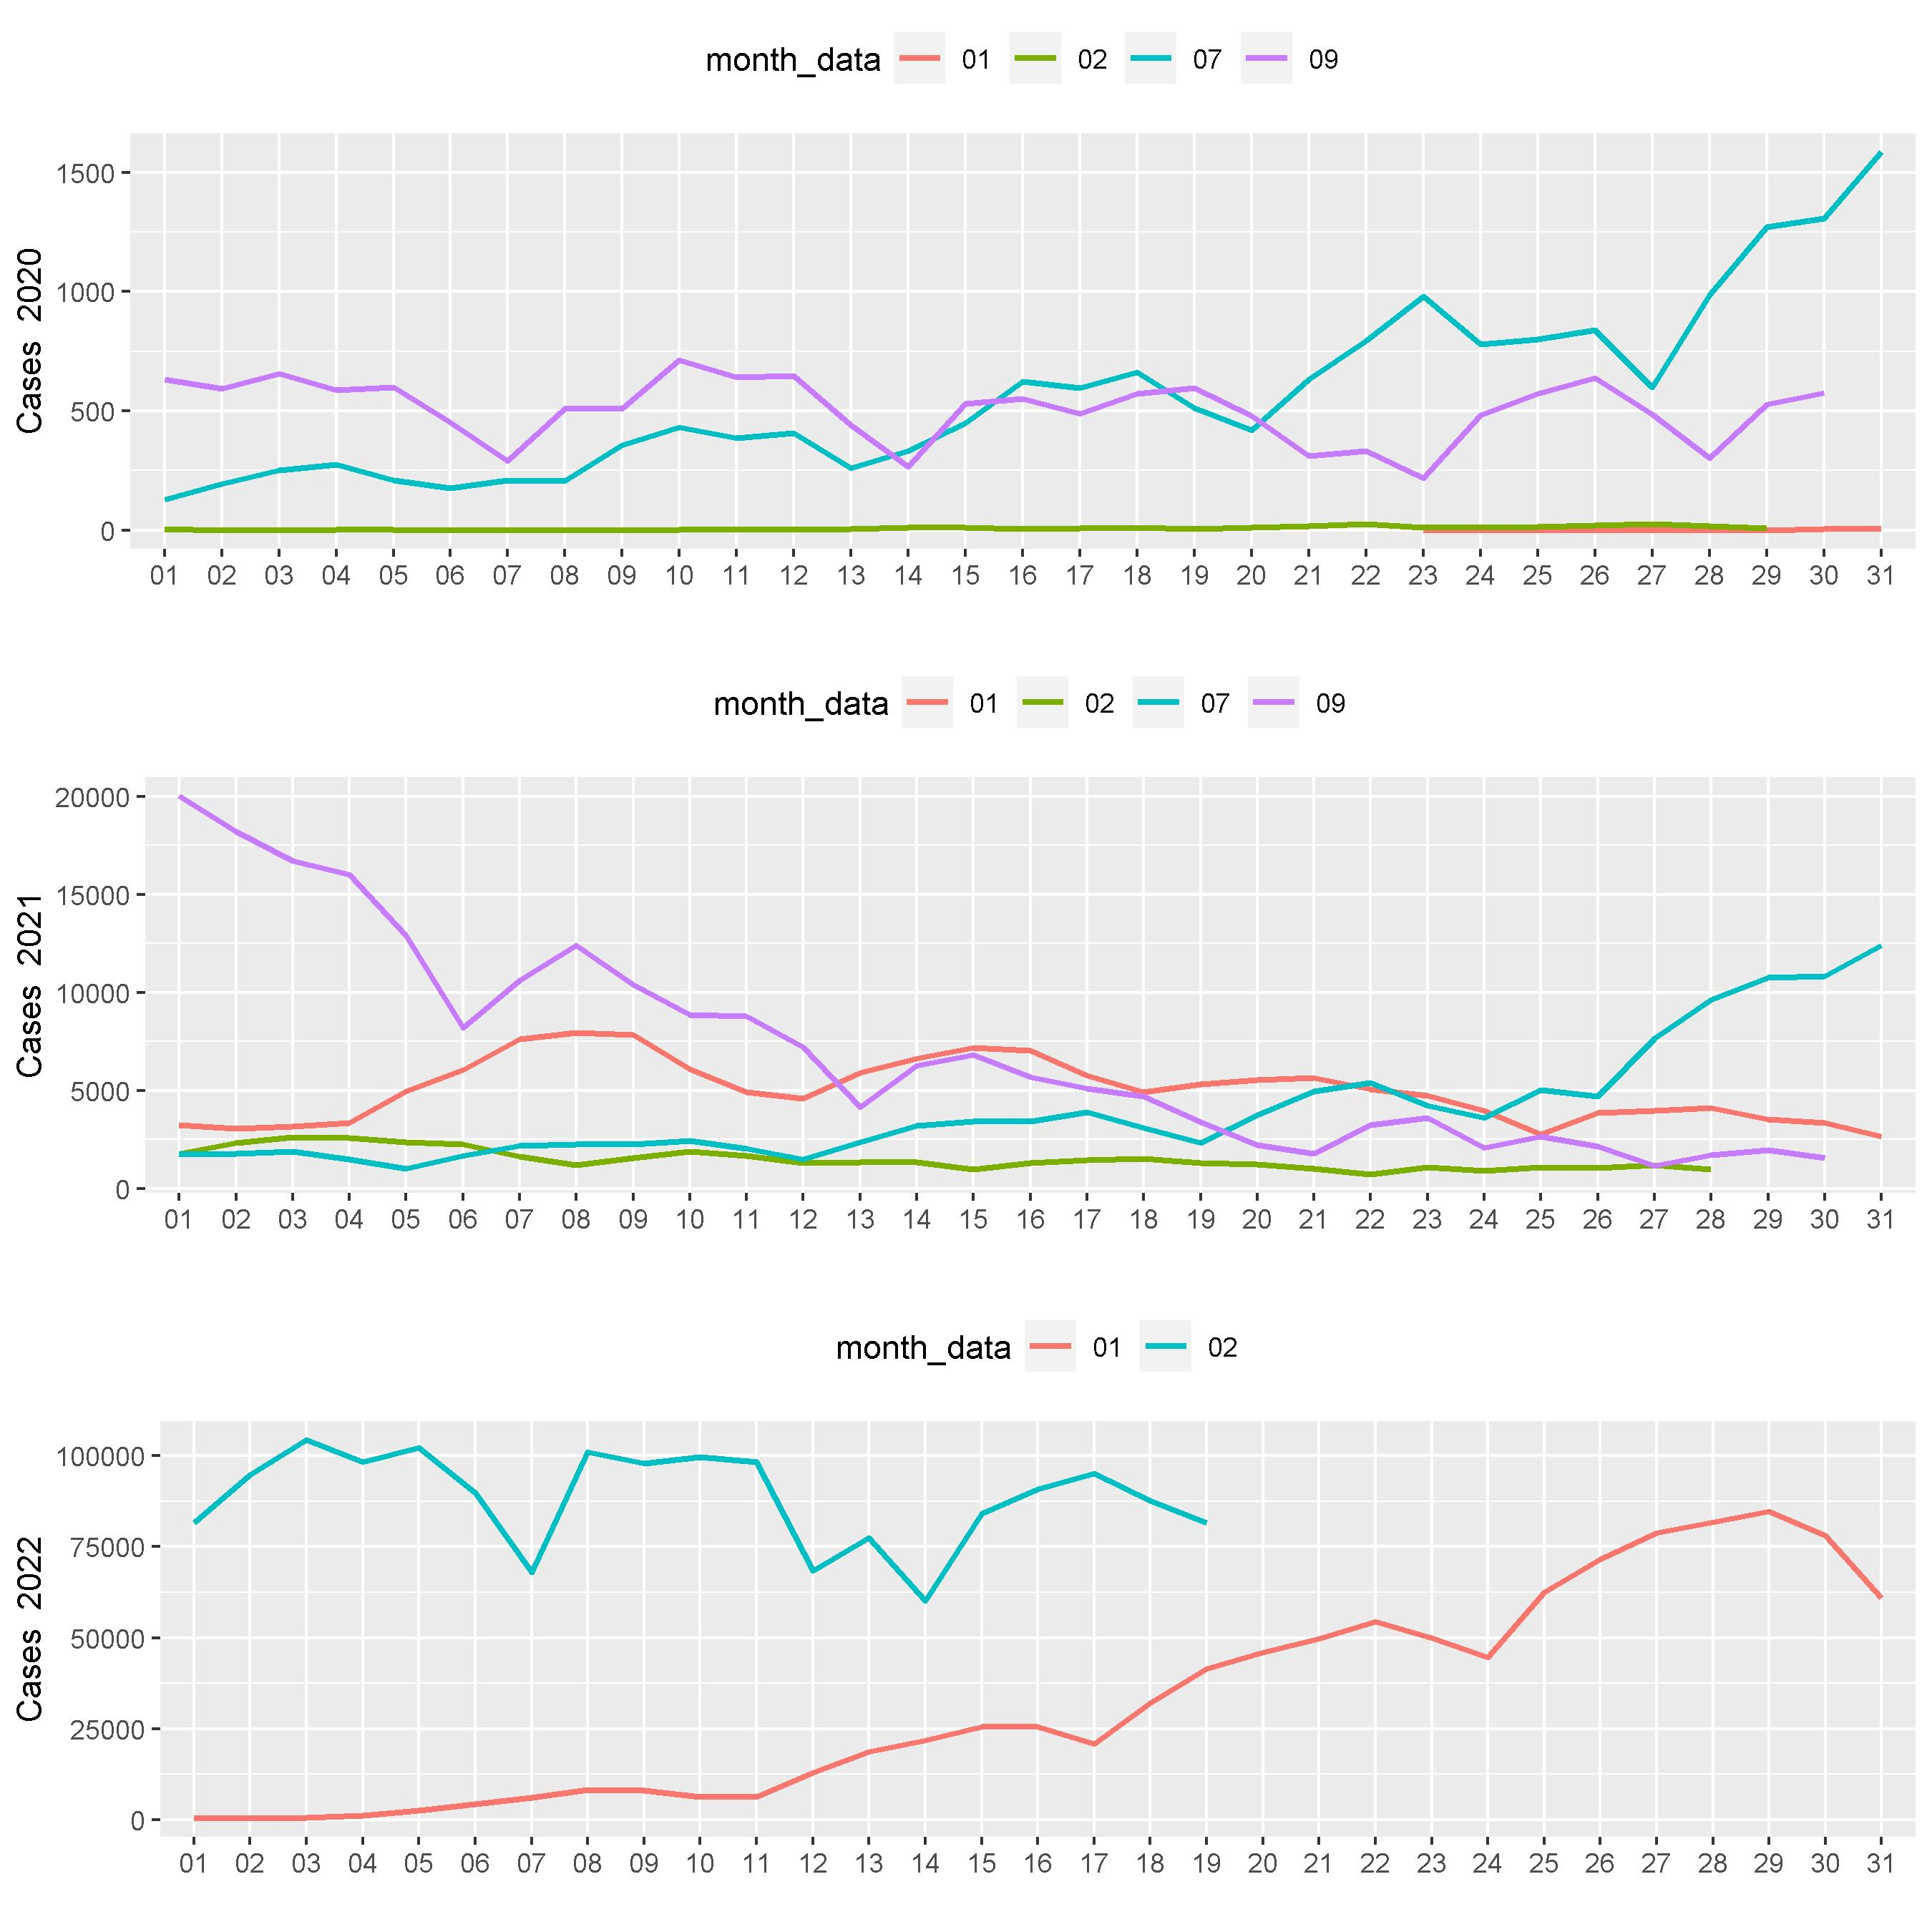
\includegraphics[scale = 0.28]{Images/V/v1 Japan .jpeg}
		     \caption{Output v1: Biểu đồ thể hiện thu thập dữ liệu nhiễm bệnh của Nhật Bản}
		\end{center}
		\end{figure}
\end{frame}

\begin{frame}[fragile]
\frametitle{5.  Nhiệm vụ}
v) \textcolor{red}{Nhóm câu hỏi liên quan đến trực quan dữ liệu theo thời gian là tháng}\\
    2) Biểu đồ thể hiện thu thập dữ liệu tử vong cho từng tháng
    	\begin{lstlisting}[frame=single,basicstyle=\tiny] 
country_chart("Vietnam","line_chart","2_1_7_9","deaths","v2")
country_chart("Japan","line_chart","2_1_7_9","deaths","v2")
country_chart("Indonesia","line_chart","2_1_7_9","deaths","v2")
		\end{lstlisting}	
\end{frame}

\begin{frame}[fragile]
\frametitle{5.  Nhiệm vụ}
v) \textcolor{red}{Nhóm câu hỏi liên quan đến trực quan dữ liệu theo thời gian là tháng}\\
    2) Biểu đồ thể hiện thu thập dữ liệu tử vong cho từng tháng
	\begin{figure}[h!]
	\begin{center}
		    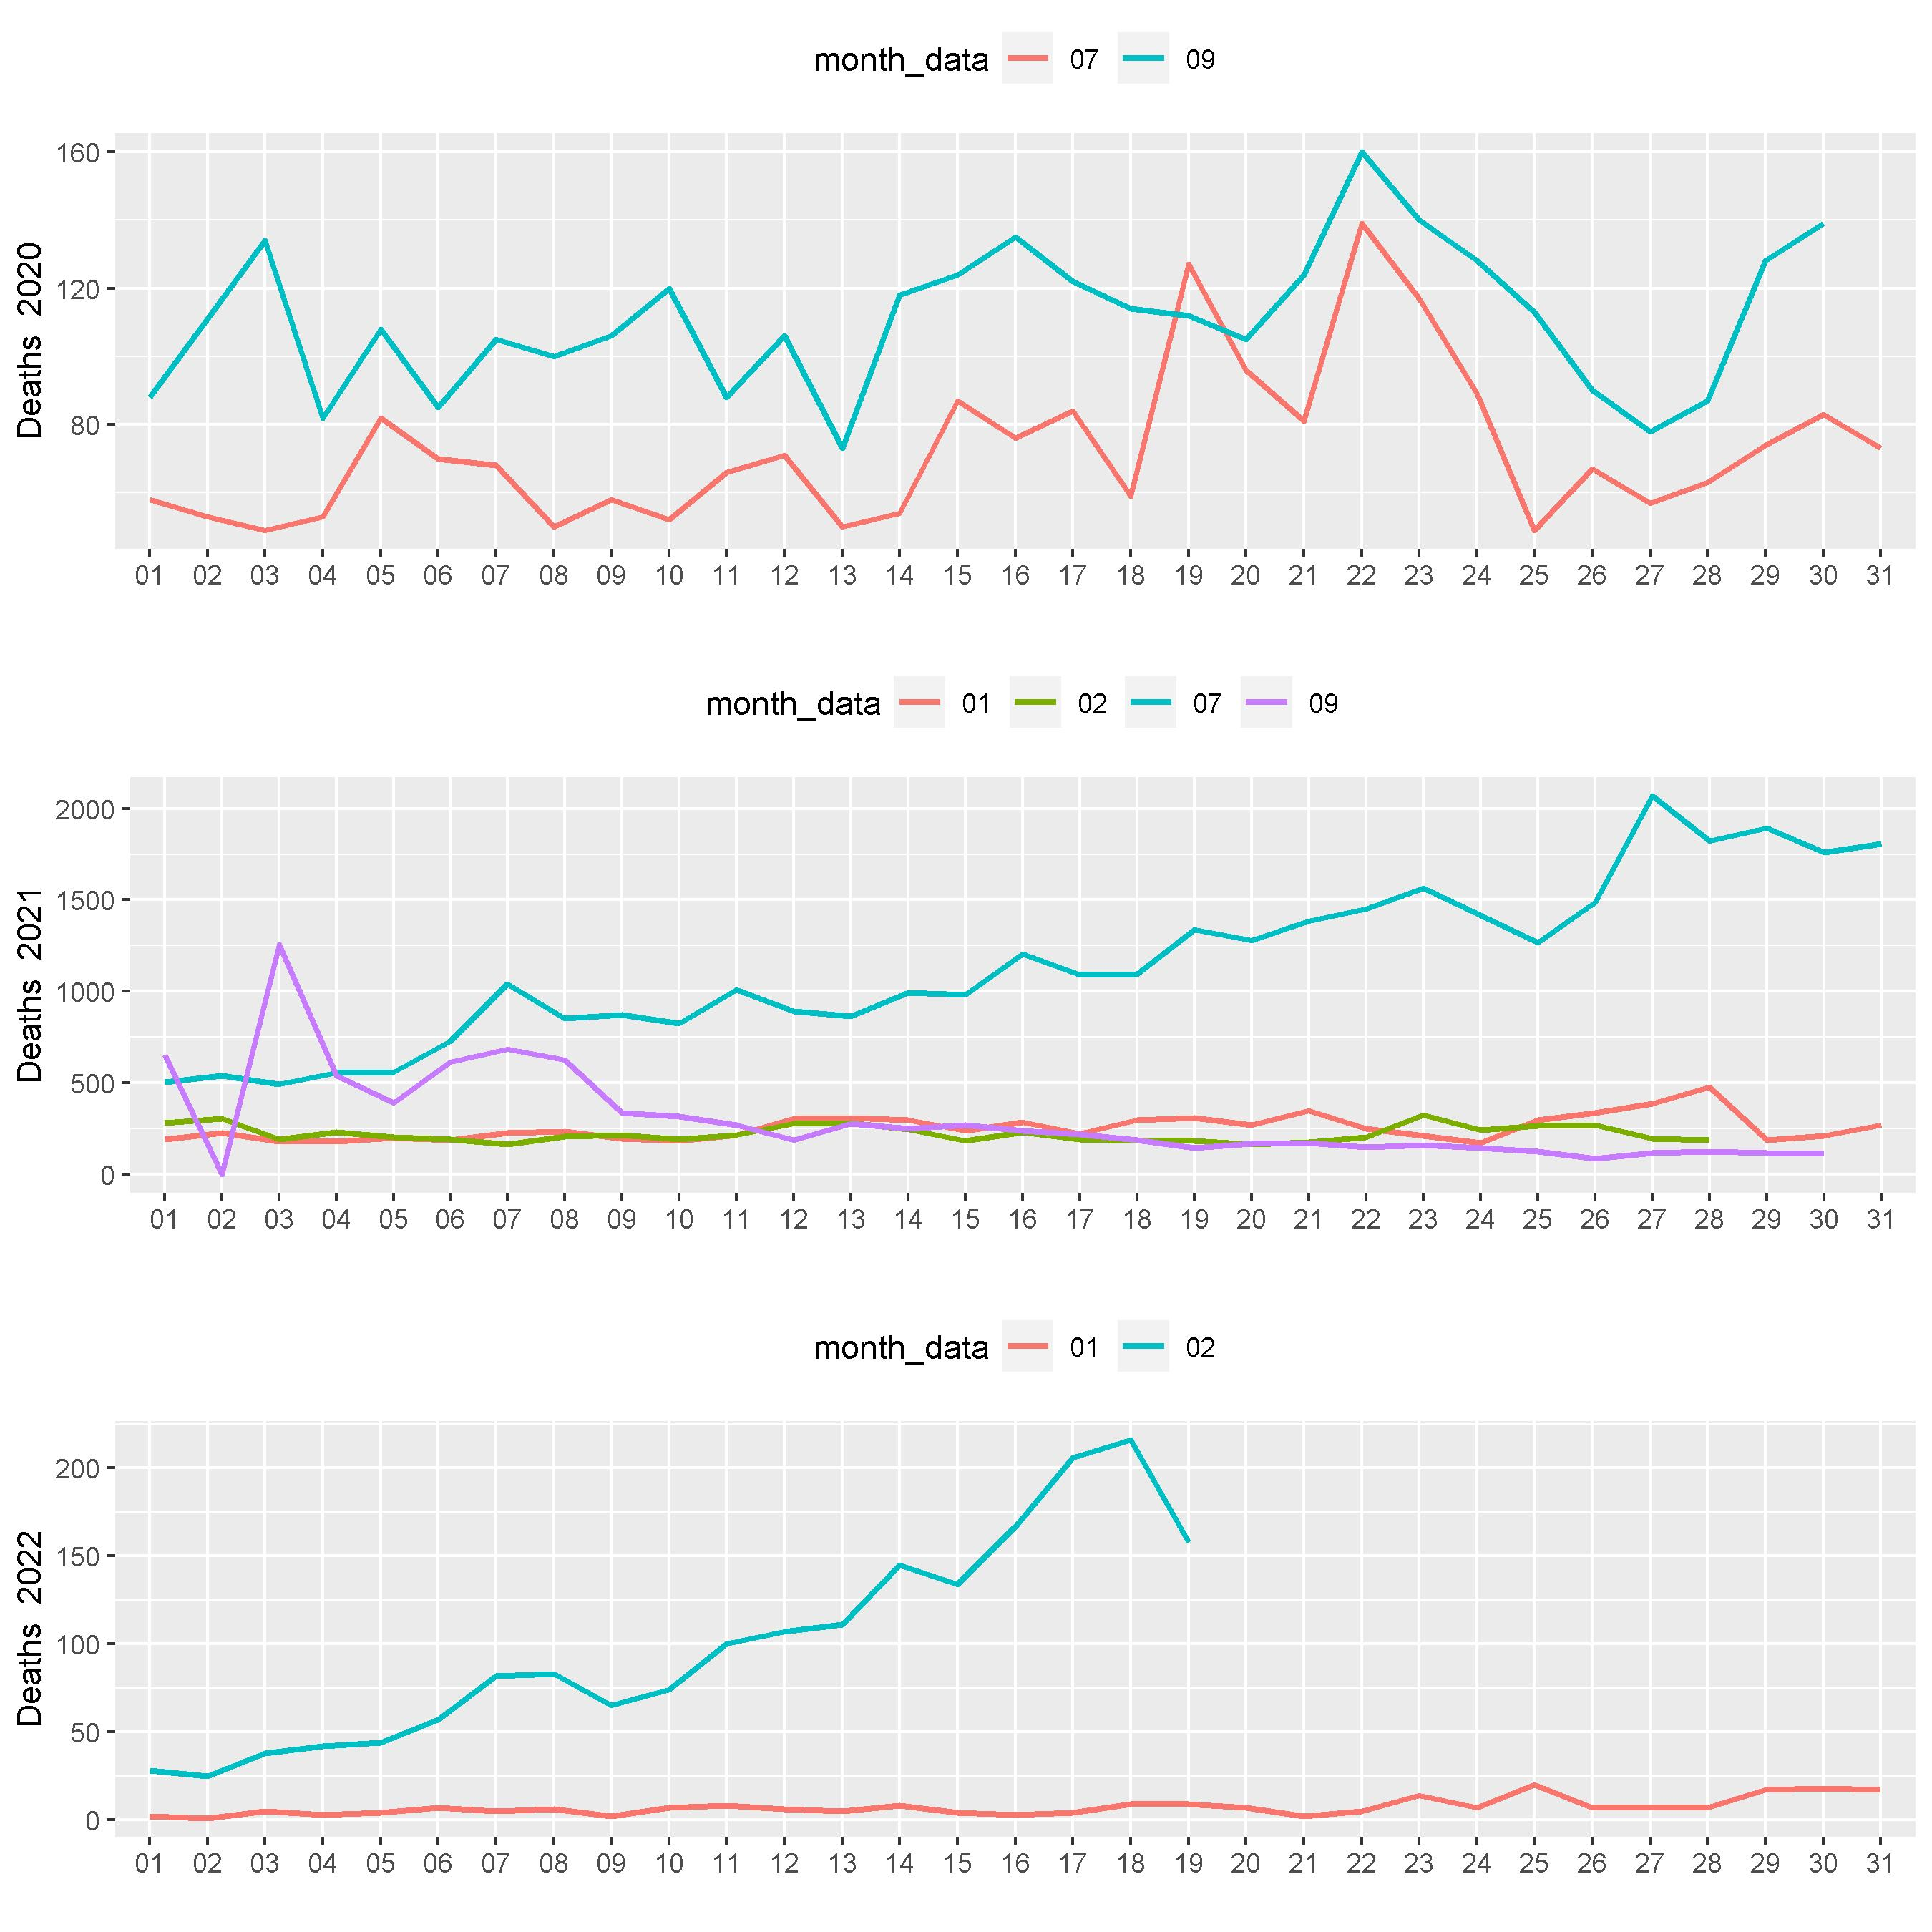
\includegraphics[scale = 0.28]{Images/V/v2 Indonesia .jpeg}
		     \caption{Output v2: Biểu đồ thể hiện thu thập dữ liệu tử vong của Indonesia}
		\end{center}
		\end{figure}
\end{frame}

\begin{frame}[fragile]
\frametitle{5.  Nhiệm vụ}
v) \textcolor{red}{Nhóm câu hỏi liên quan đến trực quan dữ liệu theo thời gian là tháng}\\
    2) Biểu đồ thể hiện thu thập dữ liệu tử vong cho từng tháng
	\begin{figure}[h!]
	\begin{center}
		    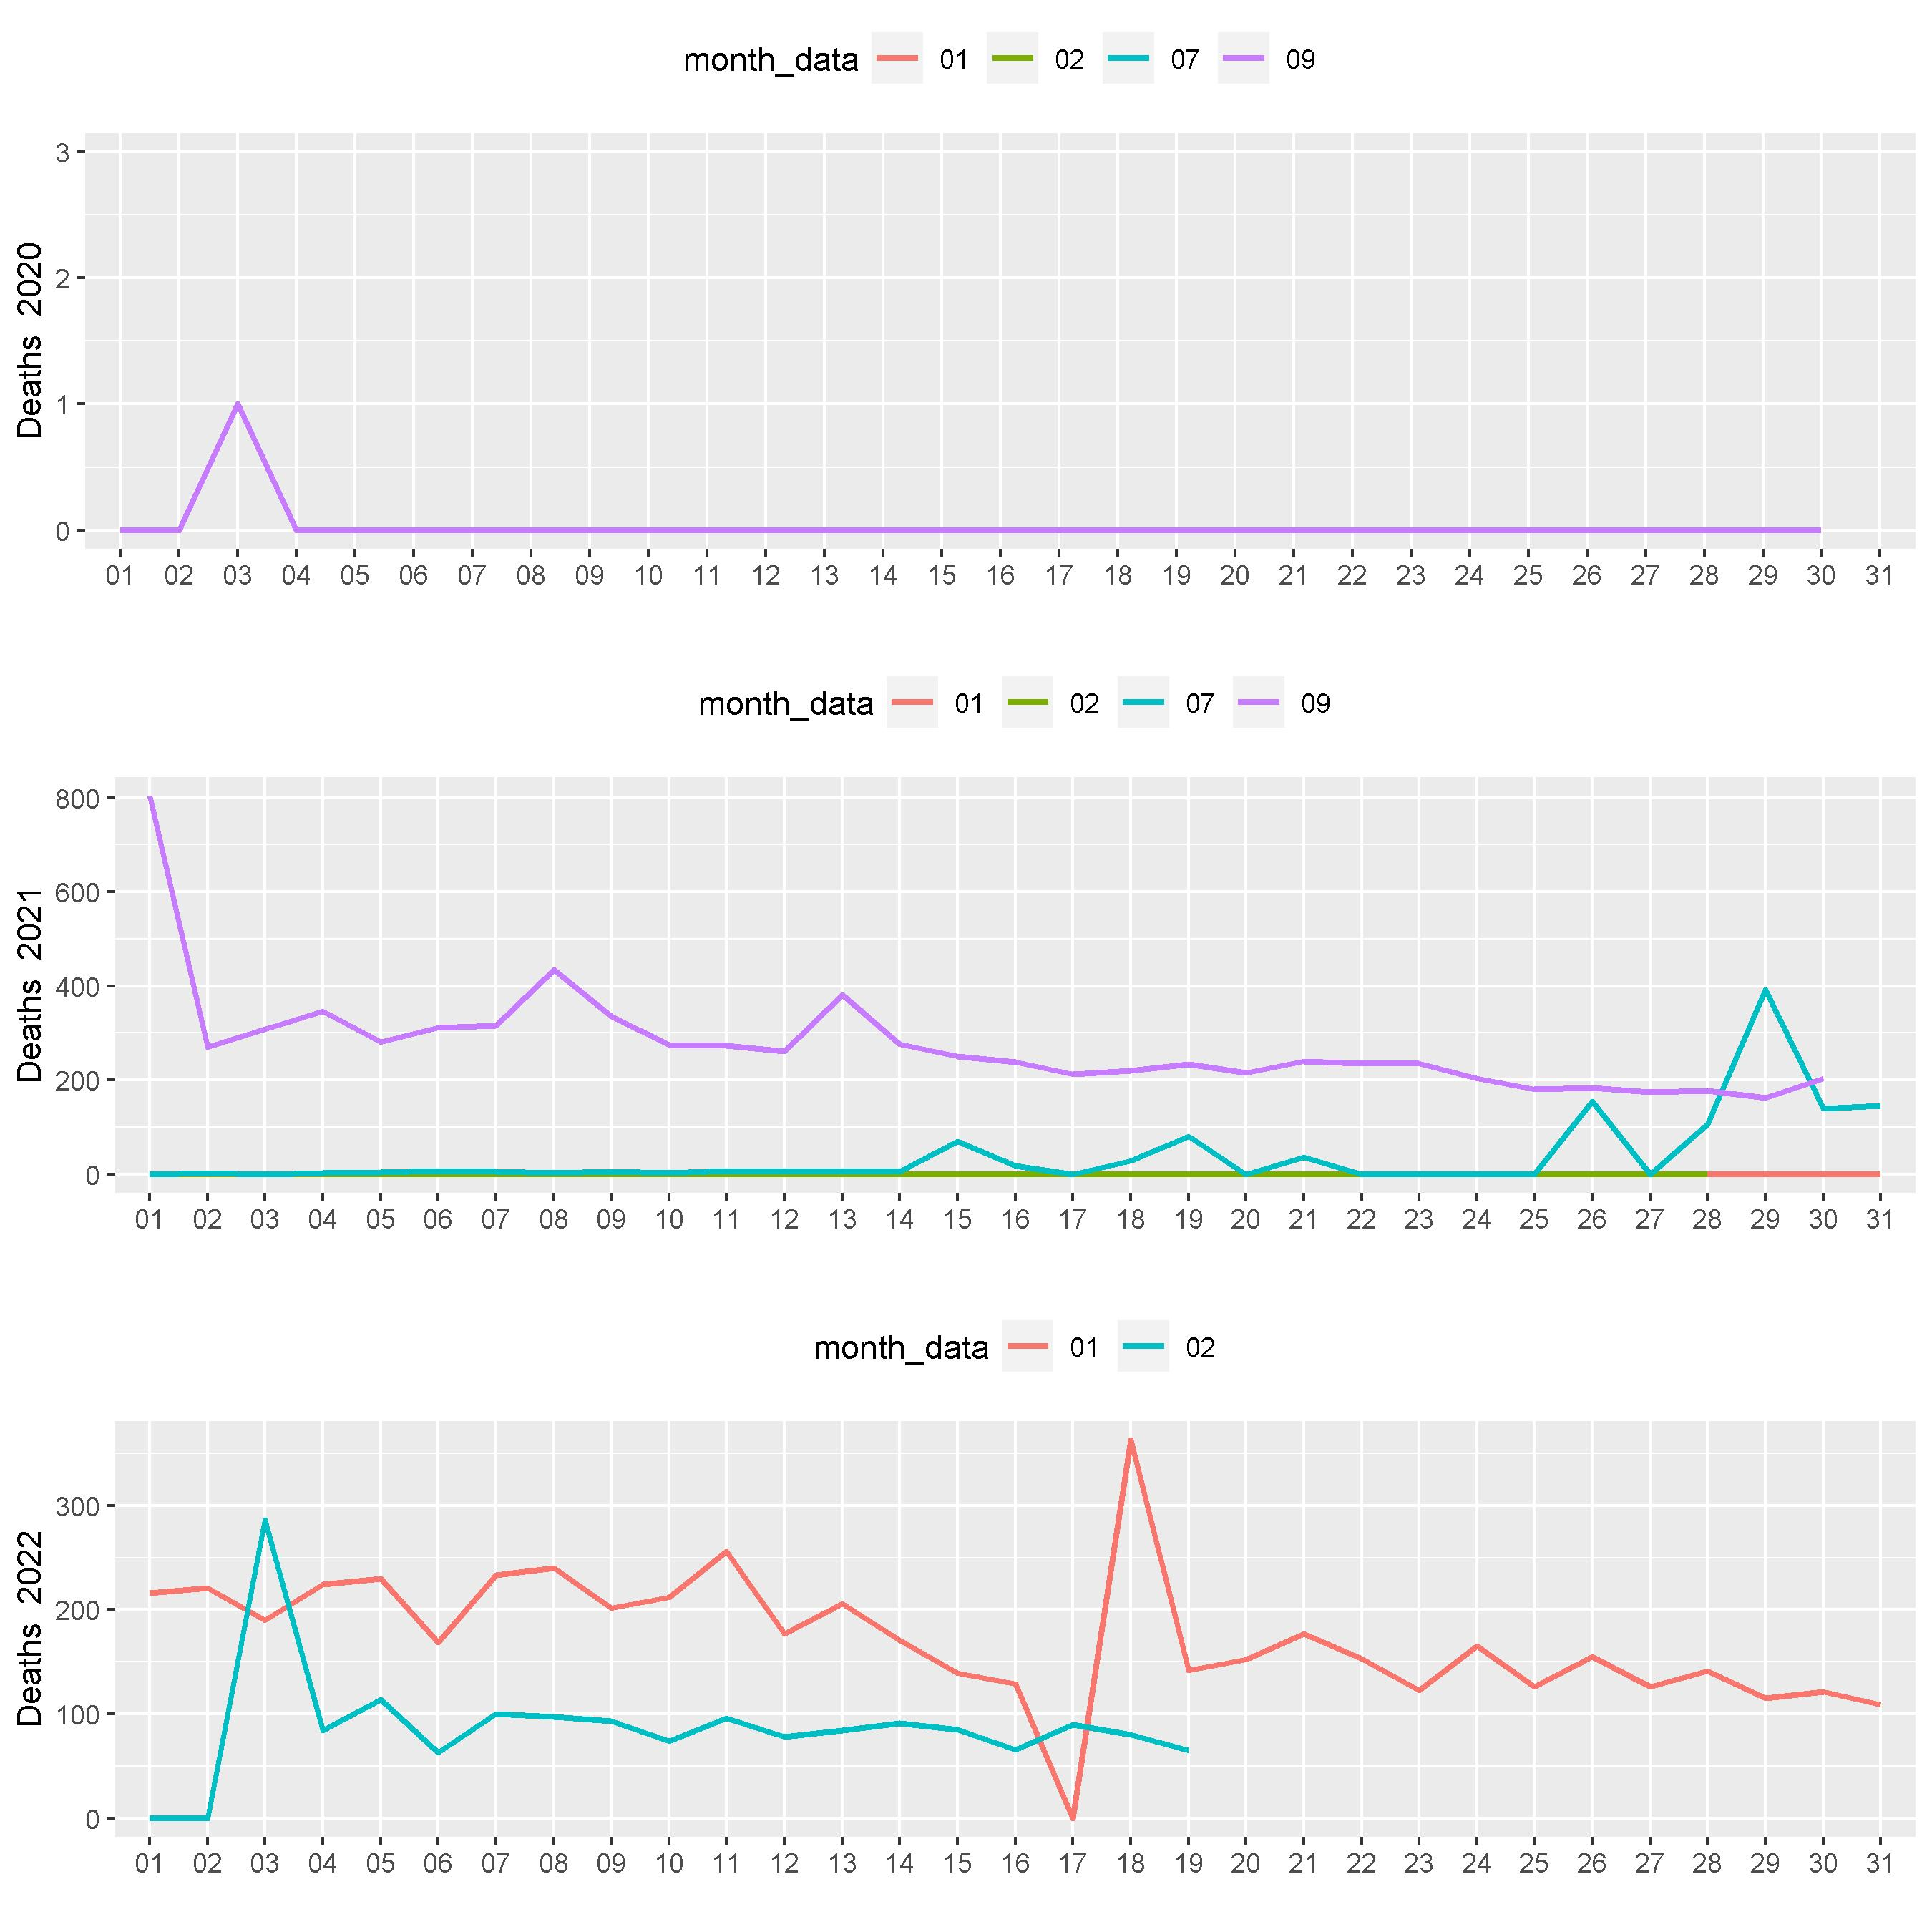
\includegraphics[scale = 0.28]{Images/V/v2 Vietnam .jpeg}
		     \caption{Output v2: Biểu đồ thể hiện thu thập dữ liệu tử vong của Việt Nam}
		\end{center}
		\end{figure}
\end{frame}

\begin{frame}[fragile]
\frametitle{5.  Nhiệm vụ}
v) \textcolor{red}{Nhóm câu hỏi liên quan đến trực quan dữ liệu theo thời gian là tháng}\\
    2) Biểu đồ thể hiện thu thập dữ liệu tử vong cho từng tháng
	\begin{figure}[h!]
	\begin{center}
		    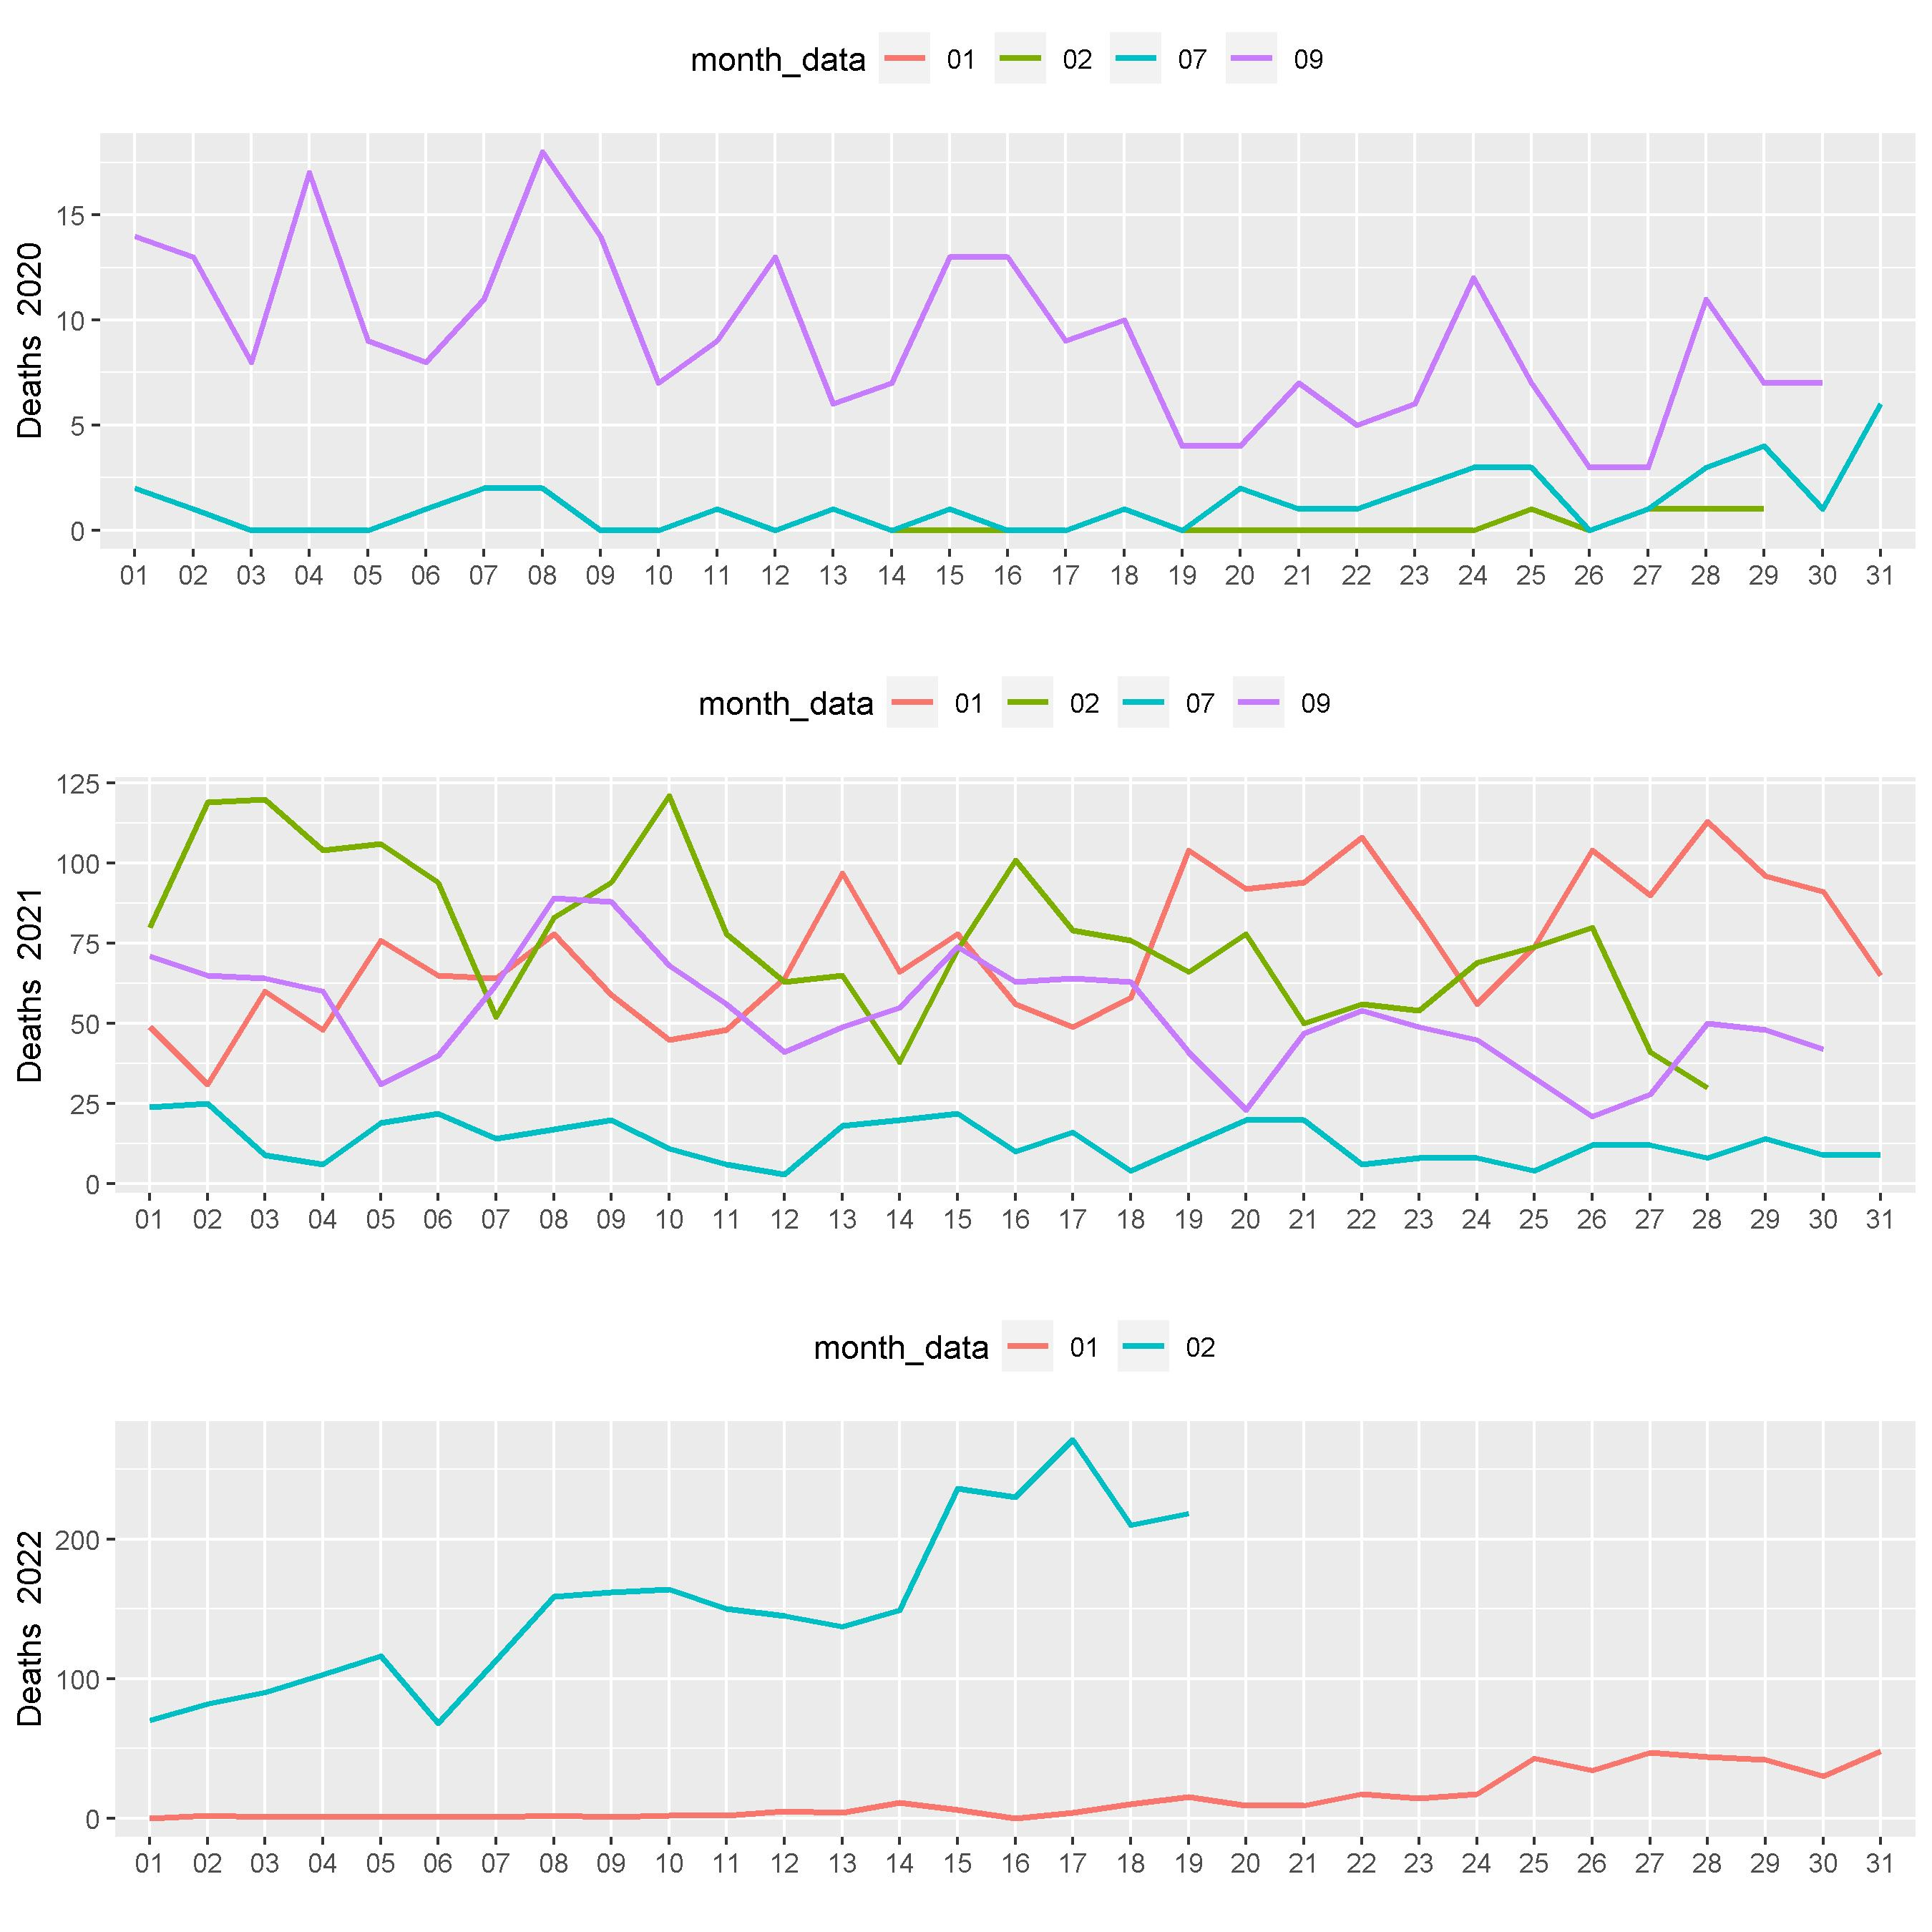
\includegraphics[scale = 0.28]{Images/V/v2 Japan .jpeg}
		     \caption{Output v2: Biểu đồ thể hiện dữ liệu tử vong của Nhật Bản}
		\end{center}
		\end{figure}
\end{frame}

\begin{frame}[fragile]
\frametitle{5.  Nhiệm vụ}
v) \textcolor{red}{Nhóm câu hỏi liên quan đến trực quan dữ liệu theo thời gian là tháng}\\
    3) Biểu đồ thể hiện thu thập dữ liệu gồm nhiễm bệnh và tử vong cho từng tháng
    	\begin{lstlisting}[frame=single,basicstyle=\tiny]  
country_chart("Vietnam","two_line","2_1_7_9","","v3")
country_chart("Japan","two_line","2_1_7_9","","v3")
country_chart("Indonesia","two_line","2_1_7_9","","v3")
		\end{lstlisting}	
\end{frame}

\begin{frame}[fragile]
\frametitle{5.  Nhiệm vụ}
v) \textcolor{red}{Nhóm câu hỏi liên quan đến trực quan dữ liệu theo thời gian là tháng}\\
    3) Biểu đồ thể hiện thu thập dữ liệu gồm nhiễm bệnh và tử vong cho từng tháng
	\begin{figure}[h!]
	\begin{center}
		    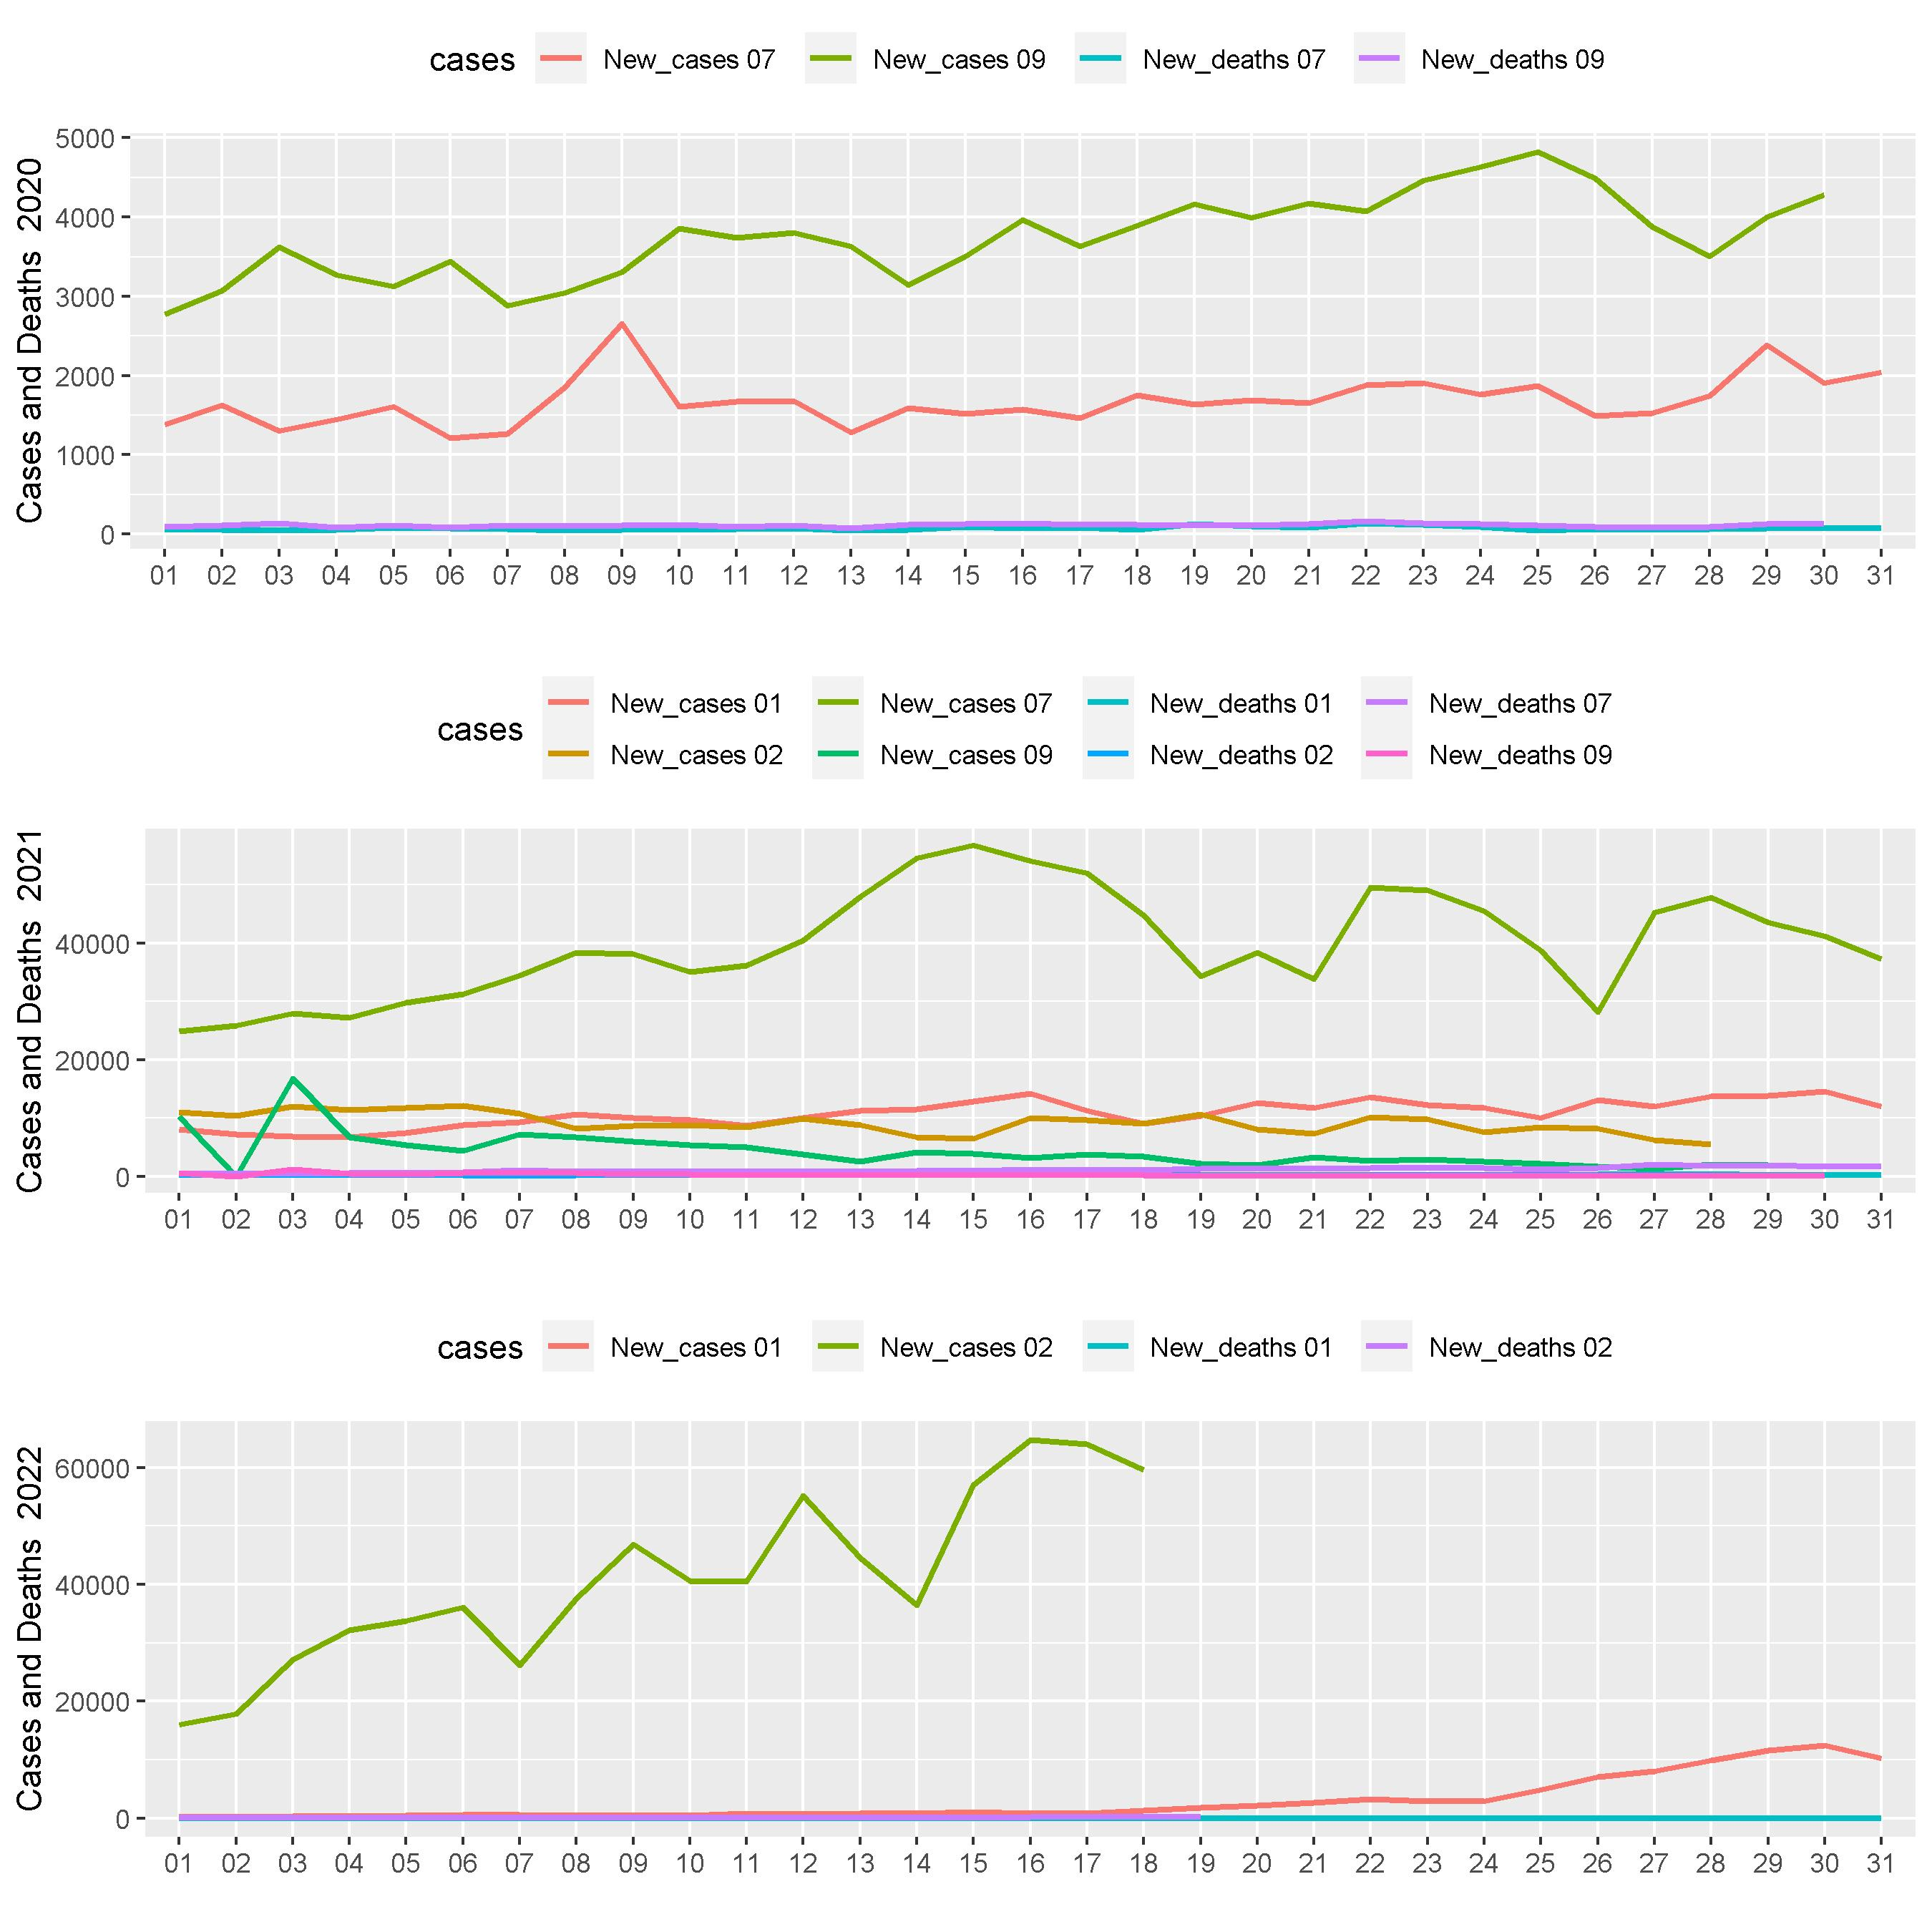
\includegraphics[scale = 0.25]{Images/V/v3 Indonesia .jpeg}
		     \caption{Output v3: Biểu đồ thể hiện thu thập dữ liệu nhiễm bệnh và tử vong của Indonesia}
		\end{center}
		\end{figure}
\end{frame}

\begin{frame}[fragile]
\frametitle{5.  Nhiệm vụ}
v) \textcolor{red}{Nhóm câu hỏi liên quan đến trực quan dữ liệu theo thời gian là tháng}\\
    3) Biểu đồ thể hiện thu thập dữ liệu gồm nhiễm bệnh và tử vong cho từng tháng
	\begin{figure}[h!]
	\begin{center}
		    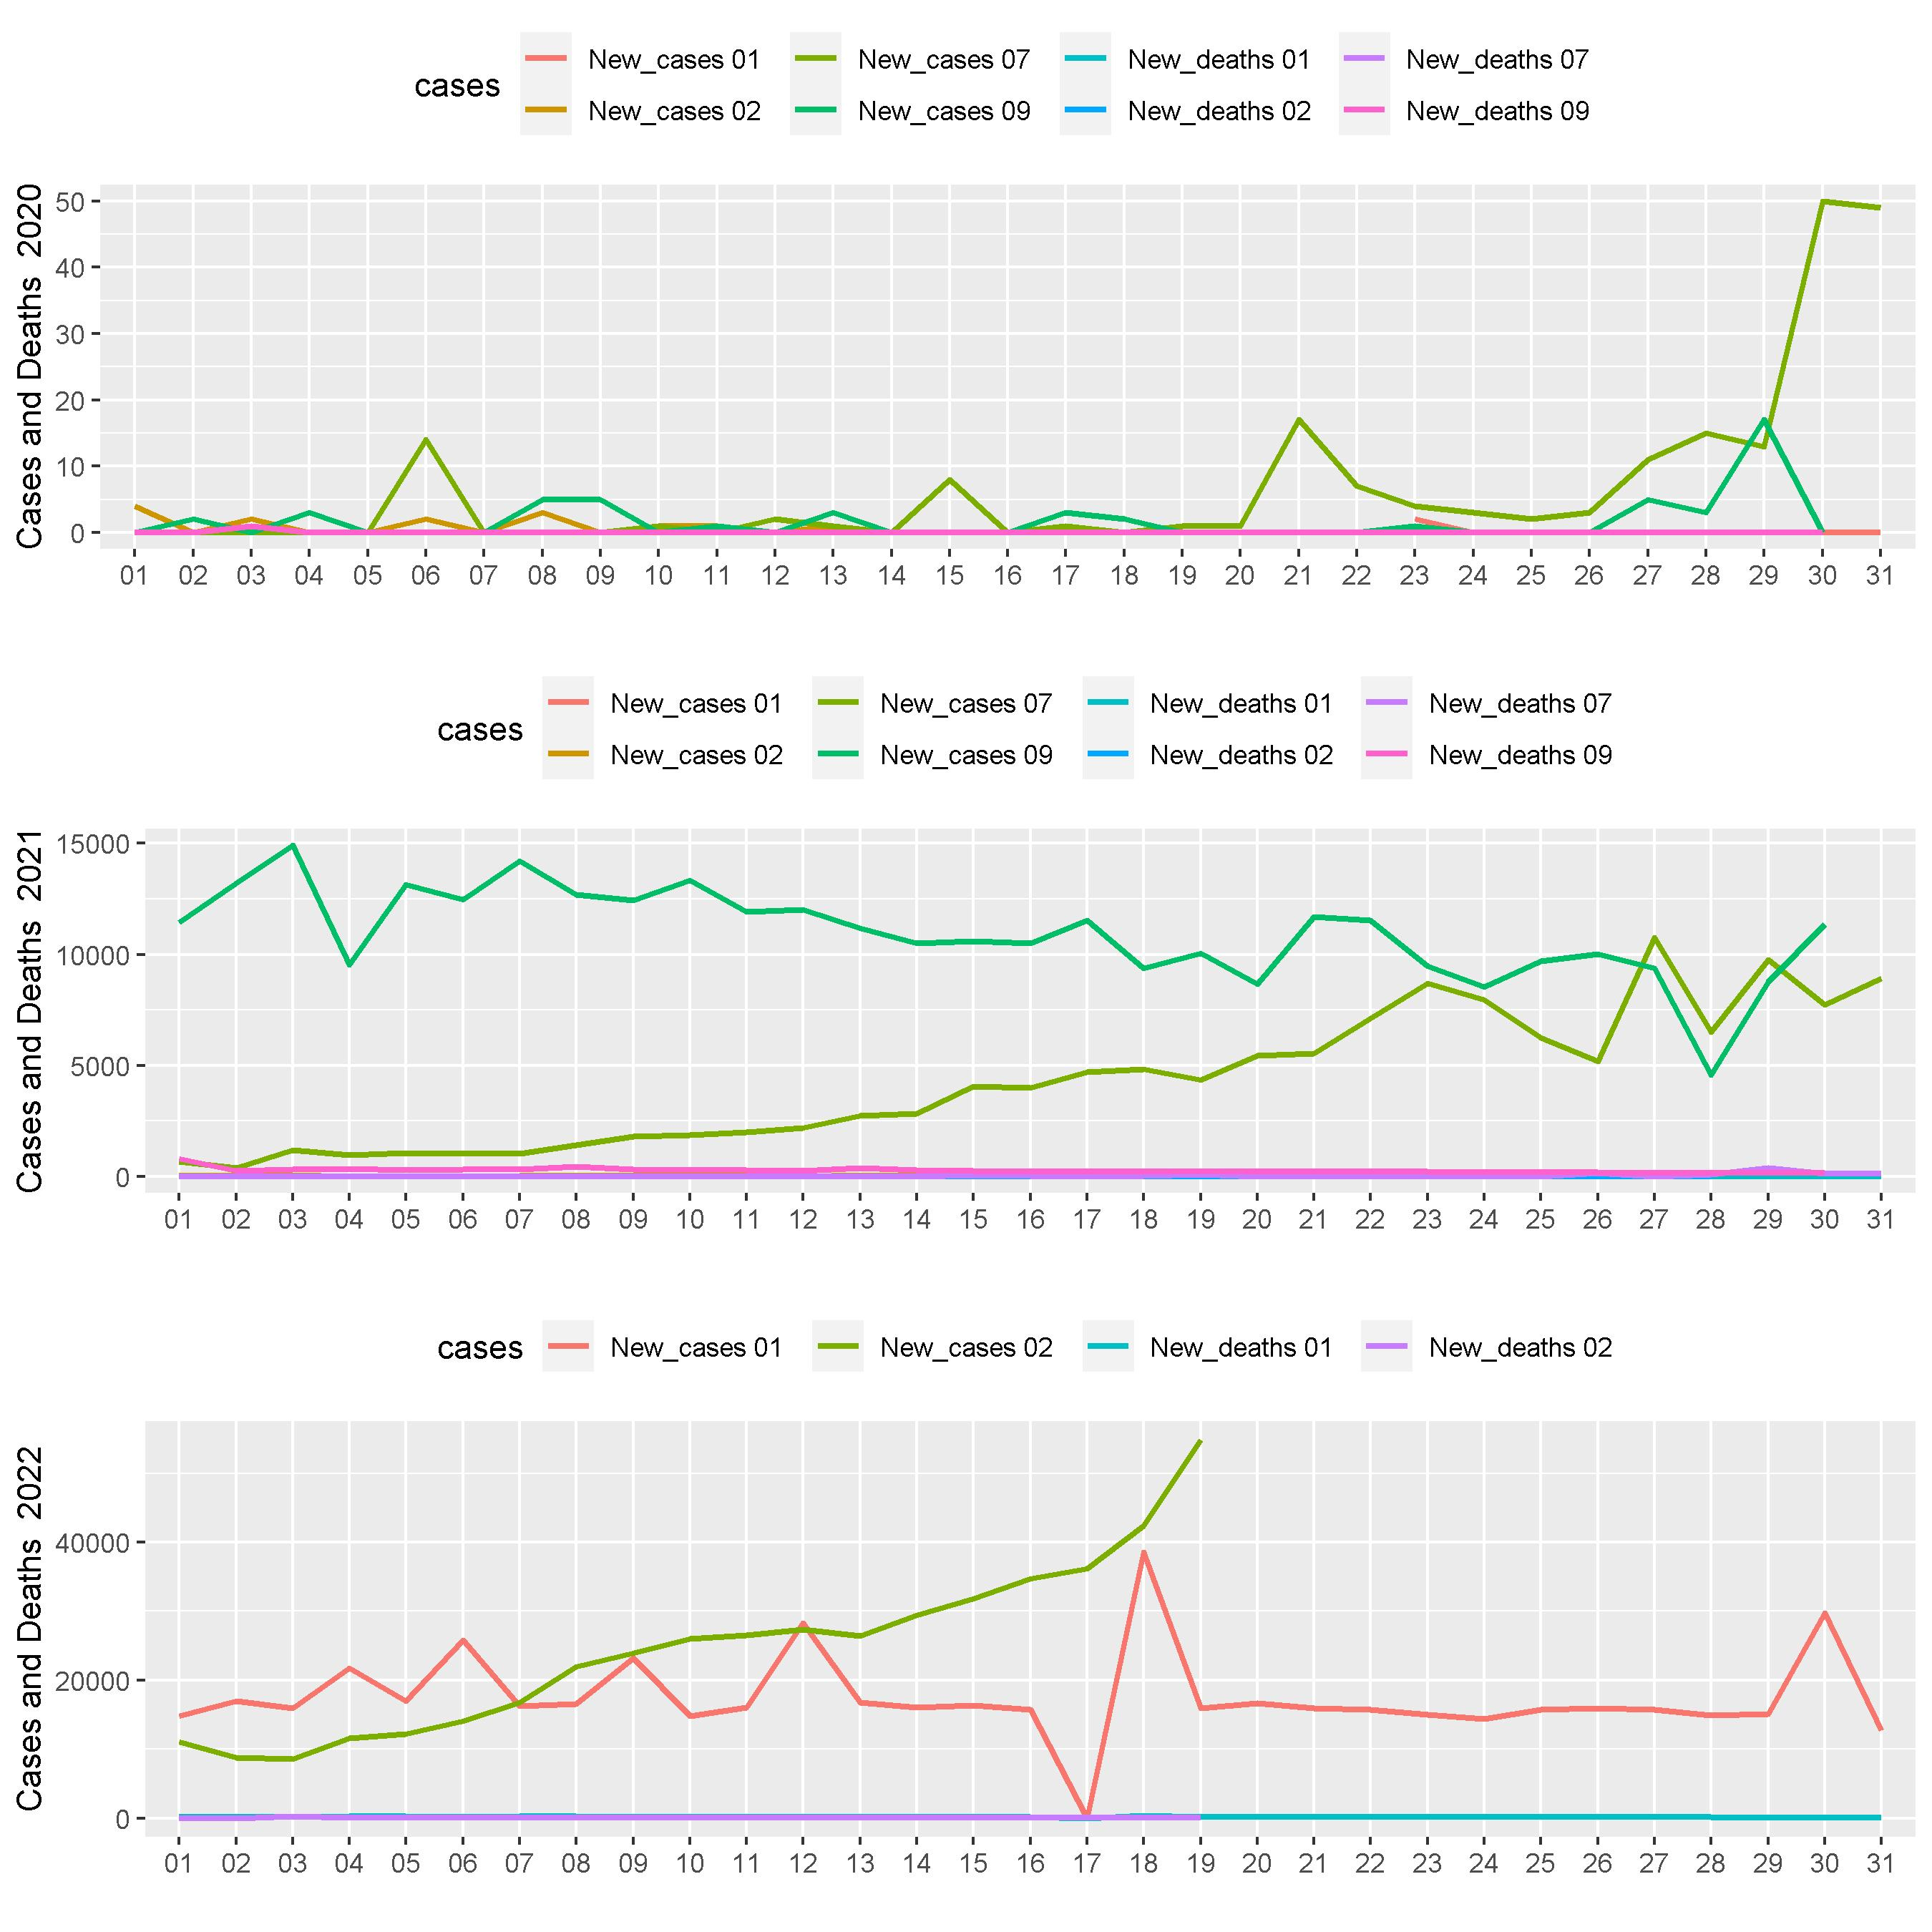
\includegraphics[scale = 0.25]{Images/V/v3 Vietnam .jpeg}
		     \caption{Output v3: Biểu đồ thể hiện thu thập dữ liệu nhiễm bệnh và tử vong của Việt Nam}
		\end{center}
		\end{figure}
\end{frame}

\begin{frame}[fragile]
\frametitle{5.  Nhiệm vụ}
v) \textcolor{red}{Nhóm câu hỏi liên quan đến trực quan dữ liệu theo thời gian là tháng}\\
    3) Biểu đồ thể hiện thu thập dữ liệu gồm nhiễm bệnh và tử vong cho từng tháng
	\begin{figure}[h!]
	\begin{center}
		    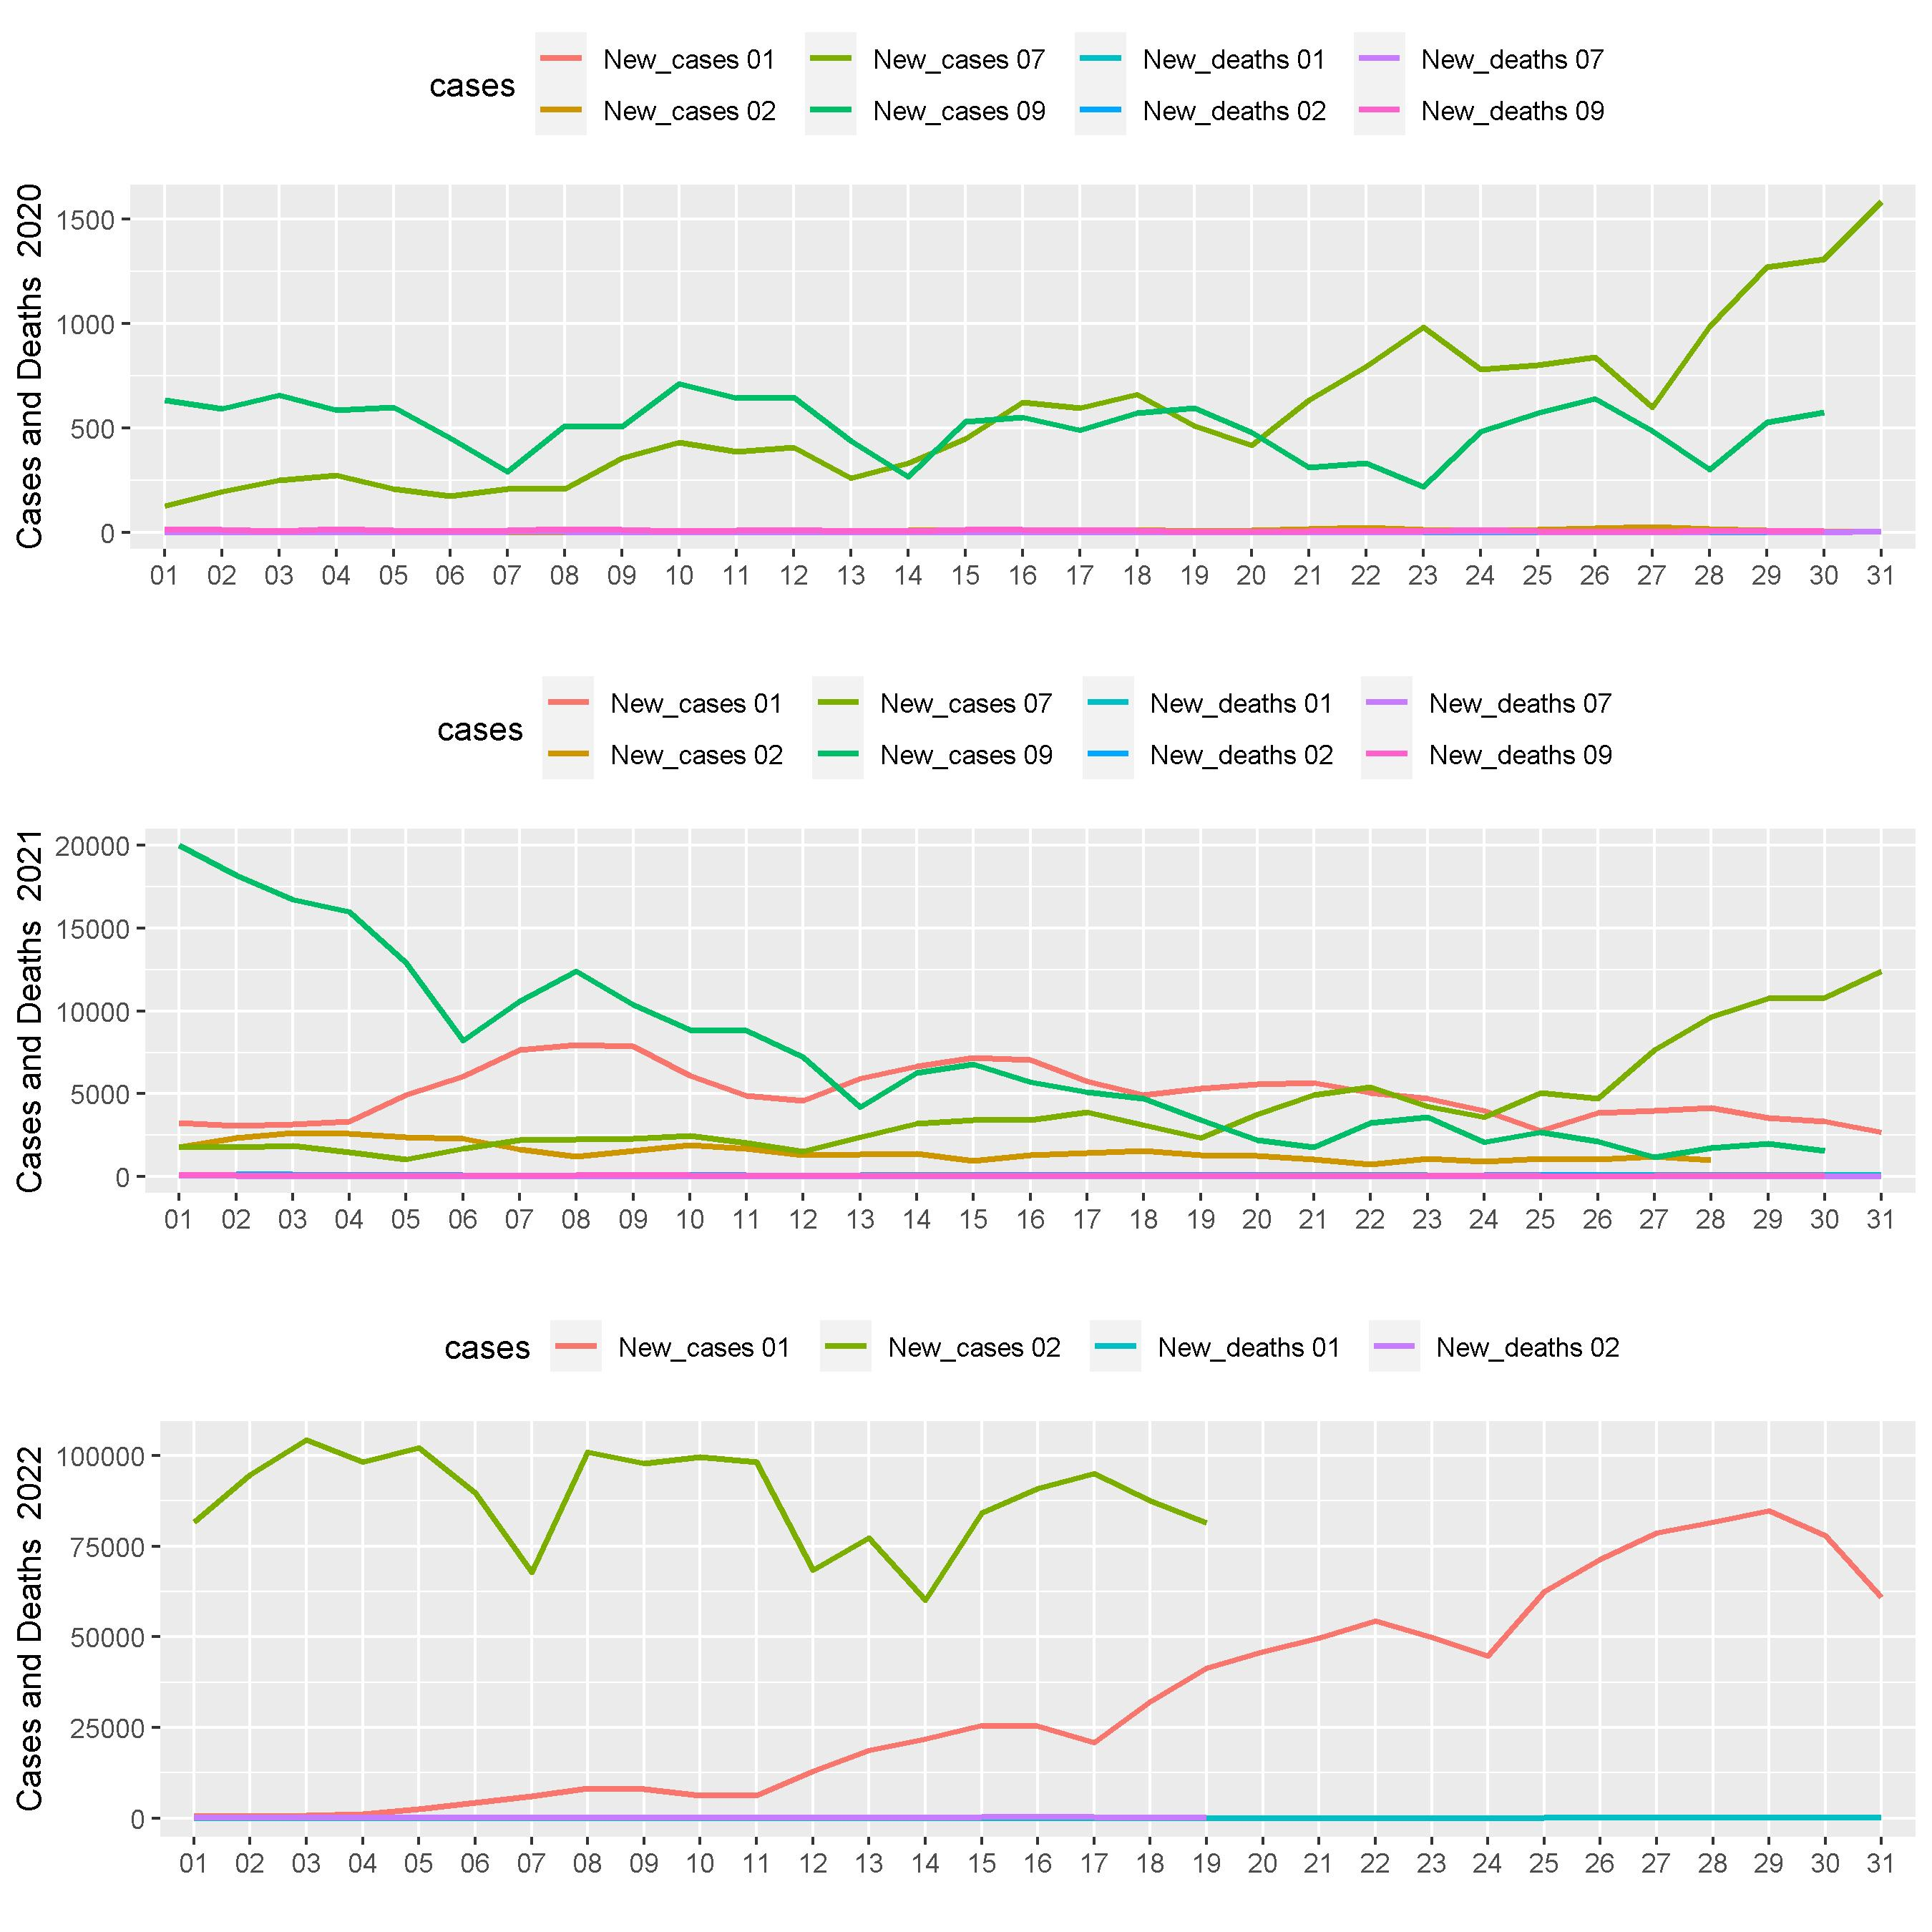
\includegraphics[scale = 0.25]{Images/V/v3 Japan .jpeg}
		     \caption{Output v3: Biểu đồ thể hiện dữ liệu nhiễm bệnh và tử vong của Nhật Bản}
		\end{center}
		\end{figure}
\end{frame}

\begin{frame}[fragile]
\frametitle{5.  Nhiệm vụ}
v) \textcolor{red}{Nhóm câu hỏi liên quan đến trực quan dữ liệu theo thời gian là tháng}\\
    4) Biểu đồ thể hiện thu thập dữ liệu nhiễm bệnh gồm 2 tháng cuối của năm
    \begin{lstlisting}[frame=single,basicstyle=\tiny]  
country_chart("Vietnam","line_chart","11_12","cases","v4")
country_chart("Japan","line_chart","11_12","cases","v4")
country_chart("Indonesia","line_chart","11_12","cases","v4")
		\end{lstlisting}
\end{frame}

\begin{frame}[fragile]
\frametitle{5.  Nhiệm vụ}
v) \textcolor{red}{Nhóm câu hỏi liên quan đến trực quan dữ liệu theo thời gian là tháng}\\
    4) Biểu đồ thể hiện thu thập dữ liệu nhiễm bệnh gồm 2 tháng cuối của năm
	\begin{figure}[h!]
	\begin{center}
		    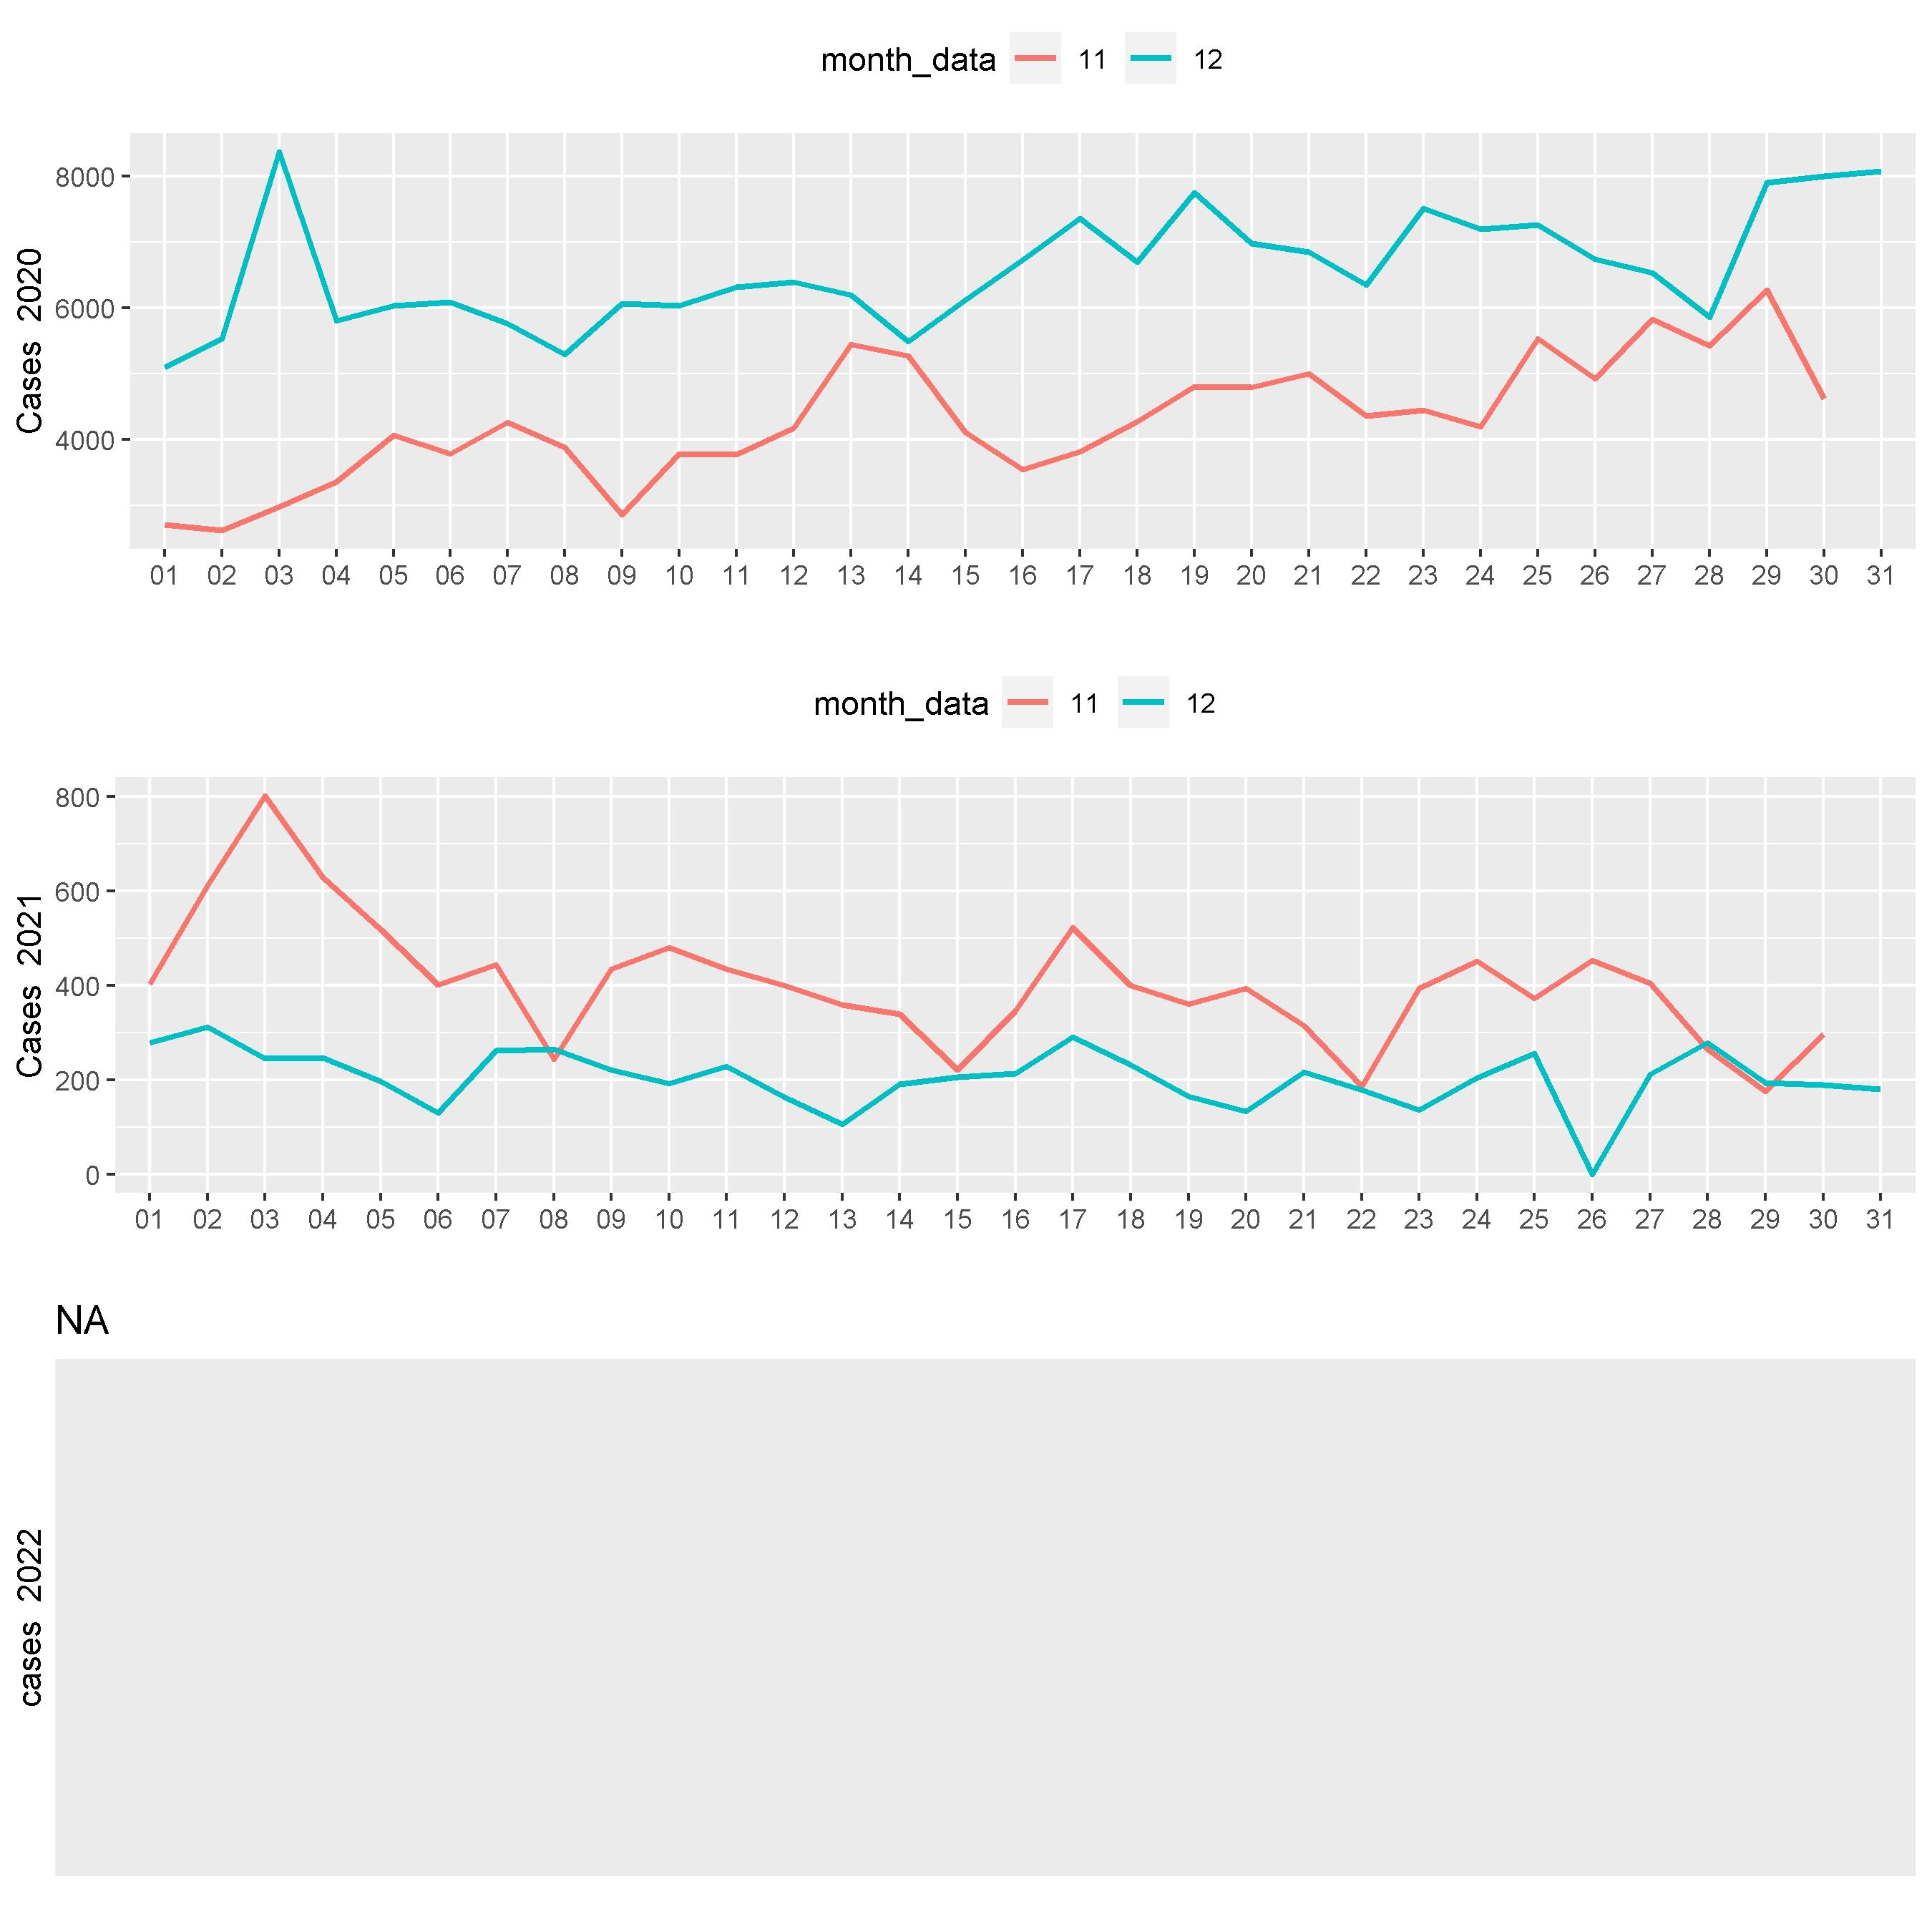
\includegraphics[scale = 0.25]{Images/V/v4 Indonesia .jpeg}
		     \caption{Output v4: Biểu đồ thể thu thập dữ liệu nhiễm bệnh theo 2 tháng cuối Indonesia}
		\end{center}
		\end{figure}
\end{frame}

\begin{frame}[fragile]
\frametitle{5.  Nhiệm vụ}
v) \textcolor{red}{Nhóm câu hỏi liên quan đến trực quan dữ liệu theo thời gian là tháng}\\
    4) Biểu đồ thể hiện thu thập dữ liệu nhiễm bệnh gồm 2 tháng cuối của năm
	\begin{figure}[h!]
	\begin{center}
		    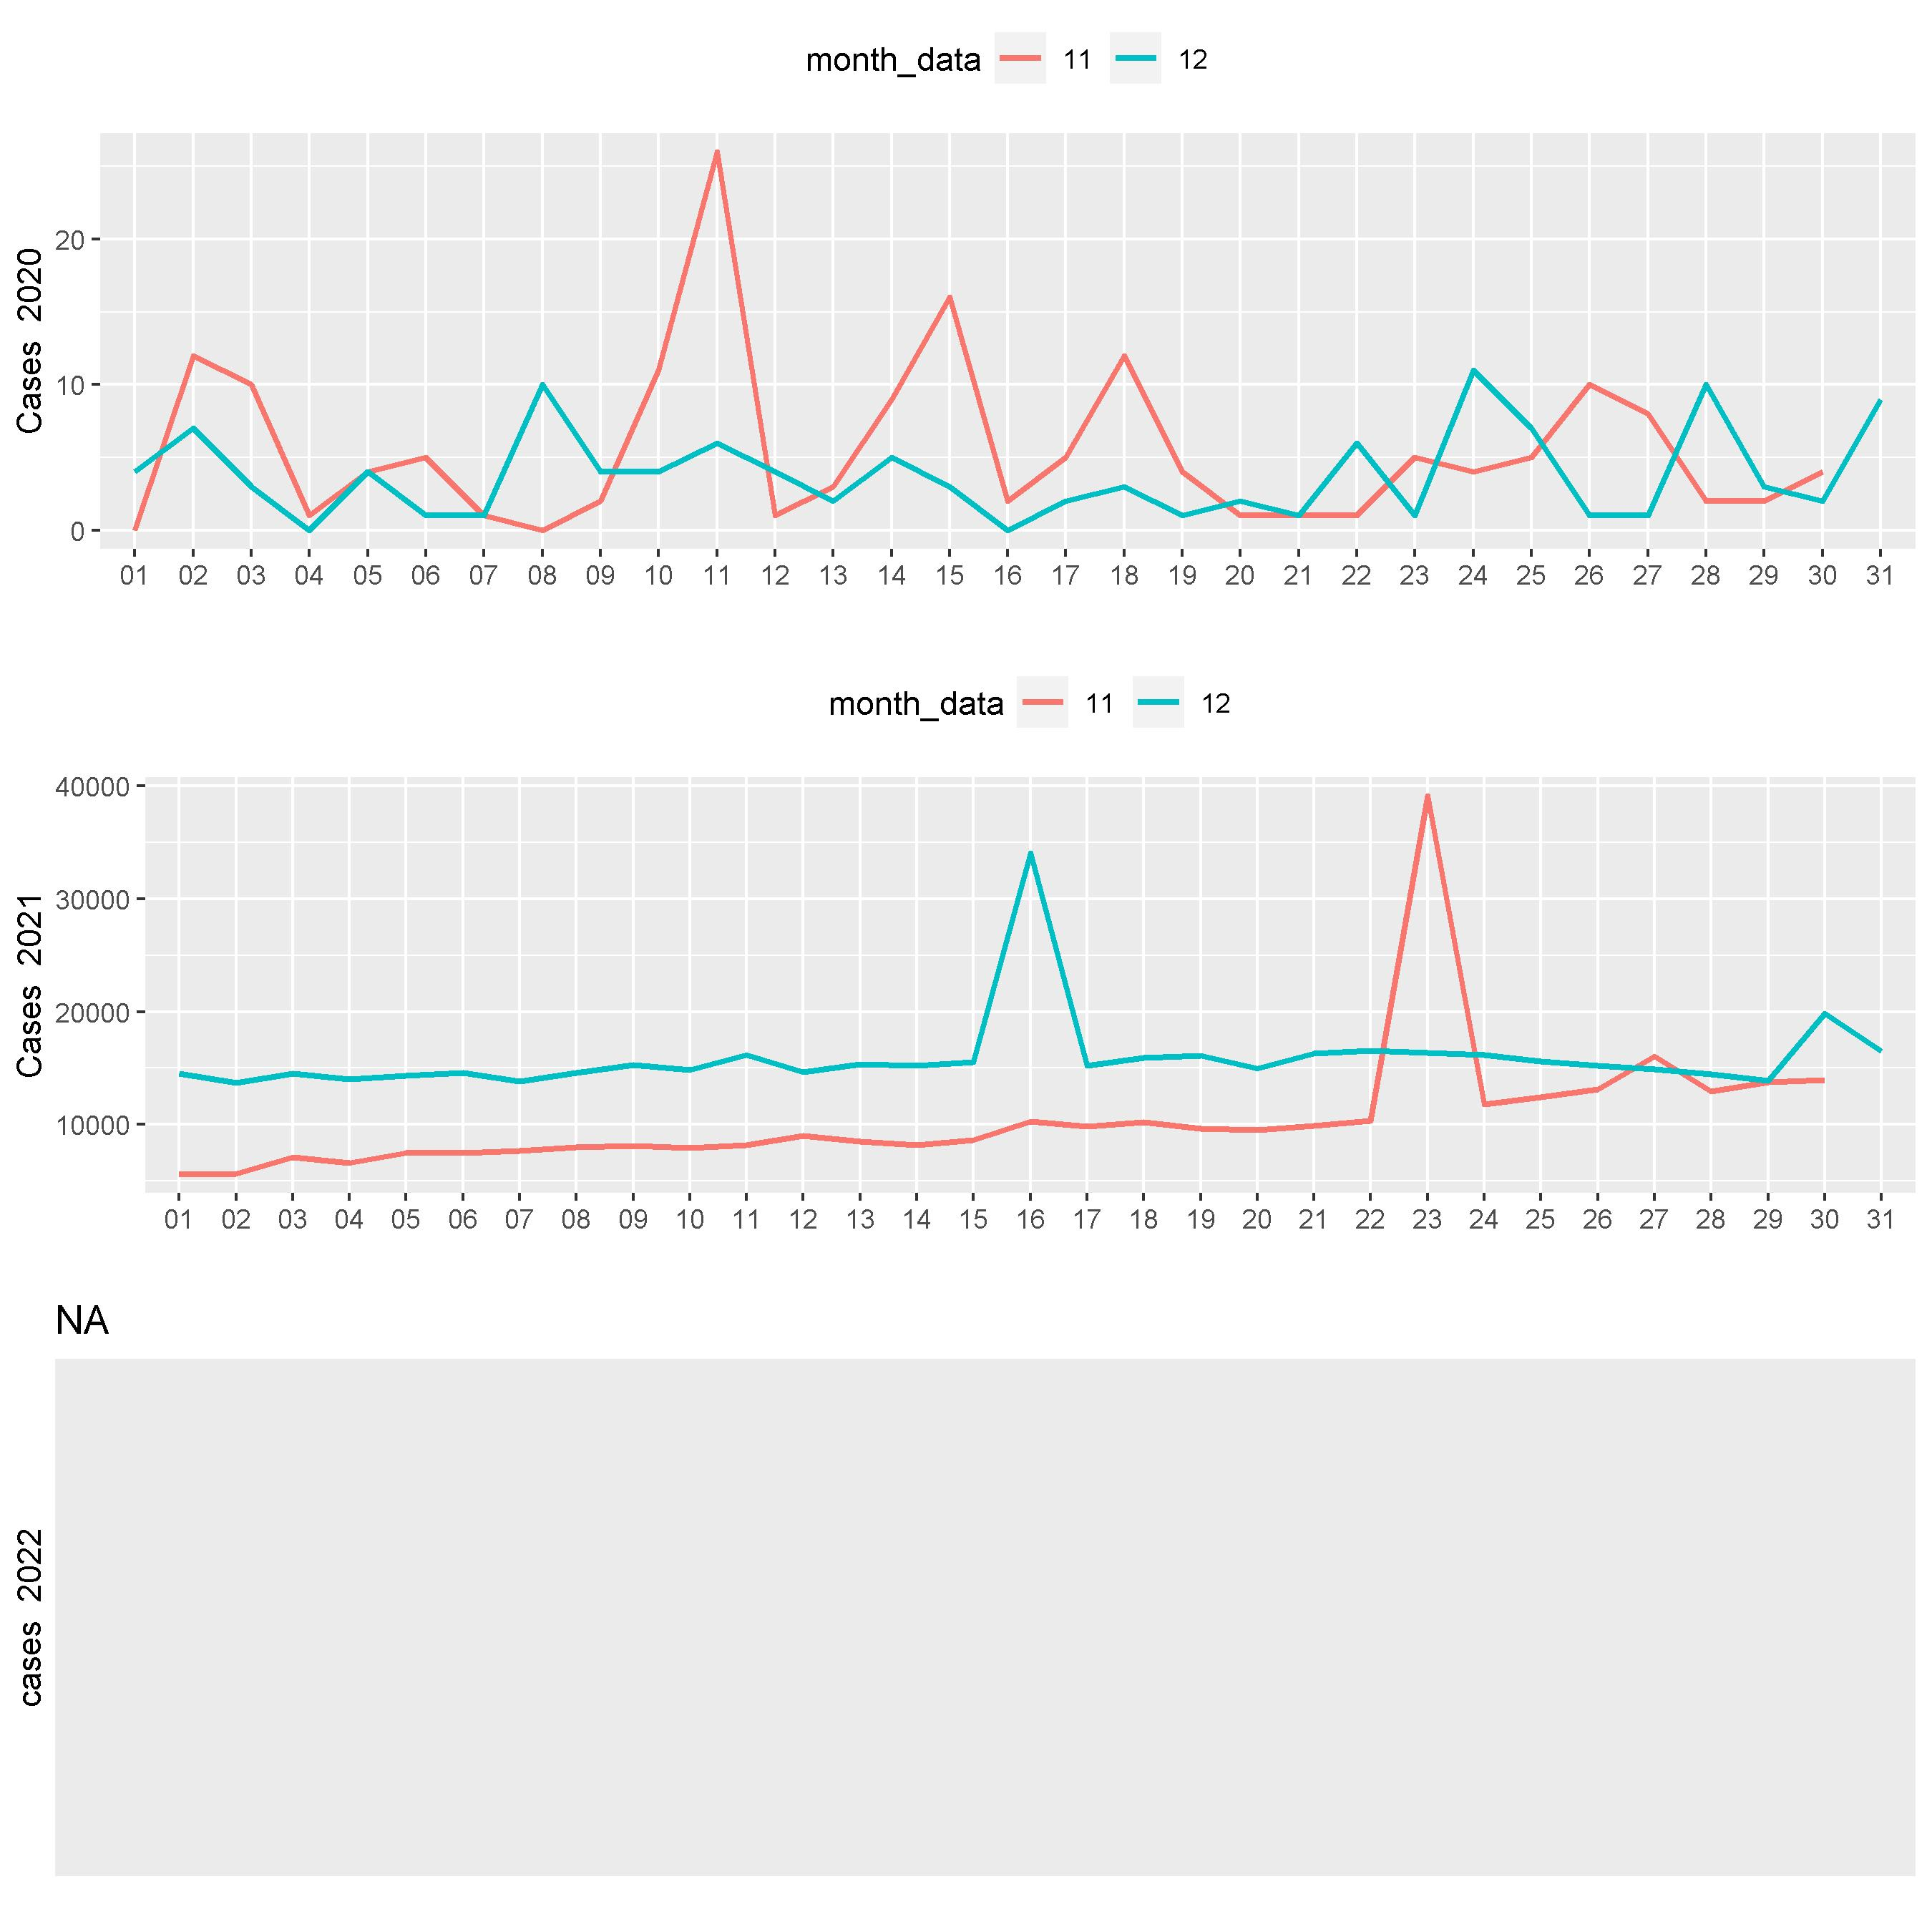
\includegraphics[scale = 0.25]{Images/V/v4 Vietnam .jpeg}
		     \caption{Output v4: Biểu đồ thể hiện thu thập dữ liệu nhiễm bệnh theo 2 tháng cuối của Việt Nam}
		\end{center}
		\end{figure}
\end{frame}

\begin{frame}[fragile]
\frametitle{5.  Nhiệm vụ}
v) \textcolor{red}{Nhóm câu hỏi liên quan đến trực quan dữ liệu theo thời gian là tháng}\\
    4) Biểu đồ thể hiện thu thập dữ liệu nhiễm bệnh gồm 2 tháng cuối của năm
	\begin{figure}[h!]
	\begin{center}
		    \includegraphics[scale = 0.25]{Images/V/v4 Japan .jpeg}
		     \caption{Output v4: Biểu đồ thể hiện thu thập dữ liệu nhiễm bệnh theo 2 tháng cuối Nhật Bản}
		\end{center}
		\end{figure}
\end{frame}

\begin{frame}[fragile]
\frametitle{5.  Nhiệm vụ}
v) \textcolor{red}{Nhóm câu hỏi liên quan đến trực quan dữ liệu theo thời gian là tháng}\\
    5) Biểu đồ thể hiện thu thập dữ liệu tử vong gồm 2 tháng cuối của năm
    \begin{lstlisting}[frame=single,basicstyle=\tiny]  
country_chart("Vietnam","line_chart","11_12","deaths","v5")
country_chart("Japan","line_chart","11_12","deaths","v5")
country_chart("Indonesia","line_chart","11_12","deaths","v5")
		\end{lstlisting}
\end{frame}

\begin{frame}[fragile]
\frametitle{5.  Nhiệm vụ}
v) \textcolor{red}{Nhóm câu hỏi liên quan đến trực quan dữ liệu theo thời gian là tháng}\\
    5) Biểu đồ thể hiện thu thập dữ liệu tử vong gồm 2 tháng cuối của năm
	\begin{figure}[h!]
	\begin{center}
		    \includegraphics[scale = 0.25]{Images/V/v5 Indonesia .jpeg}
		     \caption{Output v5: Biểu đồ thể thu thập dữ liệu tử vong theo 2 tháng cuối của Indonesia}
		\end{center}
		\end{figure}
\end{frame}

\begin{frame}[fragile]
\frametitle{5.  Nhiệm vụ}
v) \textcolor{red}{Nhóm câu hỏi liên quan đến trực quan dữ liệu theo thời gian là tháng}\\
    5) Biểu đồ thể hiện thu thập dữ liệu tử vong gồm 2 tháng cuối của năm
	\begin{figure}[h!]
	\begin{center}
		    \includegraphics[scale = 0.25]{Images/V/v5 Vietnam .jpeg}
		     \caption{Output v5: Biểu đồ thể thu thập dữ liệu tử vong theo 2 tháng cuối của Việt Nam}
		\end{center}
		\end{figure}
\end{frame}

\begin{frame}[fragile]
\frametitle{5.  Nhiệm vụ}
v) \textcolor{red}{Nhóm câu hỏi liên quan đến trực quan dữ liệu theo thời gian là tháng}\\
    5) Biểu đồ thể hiện thu thập dữ liệu tử vong gồm 2 tháng cuối của năm
	\begin{figure}[h!]
	\begin{center}
		    \includegraphics[scale = 0.25]{Images/V/v5 Japan .jpeg}
		     \caption{Output v5: Biểu đồ thể thu thập dữ liệu tử vong theo 2 tháng cuối của Nhật Bản}
		\end{center}
		\end{figure}
\end{frame}

\begin{frame}[fragile]
\frametitle{5.  Nhiệm vụ}
v) \textcolor{red}{Nhóm câu hỏi liên quan đến trực quan dữ liệu theo thời gian là tháng}\\
    6) Biểu đồ thể hiện thu thập dữ liệu gồm nhiễm bệnh và tử vong gồm 2 tháng cuối của năm
\begin{lstlisting}[frame = single,basicstyle=\tiny]
country_chart("Vietnam","two_line","11_12","","v6")
country_chart("Japan","two_line","11_12","","v6")
country_chart("Indonesia","two_line","11_12","","v6")
		\end{lstlisting}
\end{frame}

\begin{frame}[fragile]
\frametitle{5.  Nhiệm vụ}
v) \textcolor{red}{Nhóm câu hỏi liên quan đến trực quan dữ liệu theo thời gian là tháng}\\
    6) Biểu đồ thể hiện thu thập dữ liệu gồm nhiễm bệnh và tử vong gồm 2 tháng cuối của năm
	\begin{figure}[h!]
	\begin{center}
		    \includegraphics[scale = 0.25]{Images/V/v6 Indonesia .jpeg}
		     \caption{Output v6: Biểu đồ thể thu thập dữ liệu nhiễm bệnh và tử vong theo 2 tháng cuối của Indonesia}
		\end{center}
		\end{figure}
\end{frame}

\begin{frame}[fragile]
\frametitle{5.  Nhiệm vụ}
v) \textcolor{red}{Nhóm câu hỏi liên quan đến trực quan dữ liệu theo thời gian là tháng}\\
    6) Biểu đồ thể hiện thu thập dữ liệu gồm nhiễm bệnh và tử vong gồm 2 tháng cuối của năm
	\begin{figure}[h!]
	\begin{center}
		    \includegraphics[scale = 0.25]{Images/V/v6 Vietnam .jpeg}
		     \caption{Output v6: Biểu đồ thể thu thập dữ liệu nhiễm bệnh và tử vong theo 2 tháng cuối của Việt Nam}
		\end{center}
		\end{figure}
\end{frame}

\begin{frame}[fragile]
\frametitle{5.  Nhiệm vụ}
v) \textcolor{red}{Nhóm câu hỏi liên quan đến trực quan dữ liệu theo thời gian là tháng}\\
    6) Biểu đồ thể hiện thu thập dữ liệu gồm nhiễm bệnh và tử vong gồm 2 tháng cuối của năm
	\begin{figure}[h!]
	\begin{center}
		    \includegraphics[scale = 0.25]{Images/V/v6 Japan .jpeg}
		     \caption{Output v6: Biểu đồ thể thu thập dữ liệu nhiễm bệnh và tử vong theo 2 tháng cuối của Nhật Bản}
		\end{center}
		\end{figure}
\end{frame}

\begin{frame}[fragile]
\frametitle{5.  Nhiệm vụ}
v) \textcolor{red}{Nhóm câu hỏi liên quan đến trực quan dữ liệu theo thời gian là tháng}\\
    7) Biểu đồ thể hiện thu thập dữ liệu nhiễm bệnh tích lũy cho từng tháng
    \begin{lstlisting}[frame=single,basicstyle=\tiny]  
country_chart("Vietnam","cum","2_1_7_9","cases","v7")
country_chart("Japan","cum","2_1_7_9","cases","v7")
country_chart("Indonesia","cum","2_1_7_9","cases","v7")
		\end{lstlisting}
\end{frame}

\begin{frame}[fragile]
\frametitle{5.  Nhiệm vụ}
v) \textcolor{red}{Nhóm câu hỏi liên quan đến trực quan dữ liệu theo thời gian là tháng}\\
    7) Biểu đồ thể hiện thu thập dữ liệu nhiễm bệnh tích lũy cho từng tháng
	\begin{figure}[h!]
	\begin{center}
		    \includegraphics[scale = 0.26]{Images/V/v7 Indonesia .jpeg}
		     \caption{Output v7: Biểu đồ thể hiện thu thập dữ liệu nhiễm bệnh tích của Indonesia}
		\end{center}
		\end{figure}
\end{frame}

\begin{frame}[fragile]
\frametitle{5.  Nhiệm vụ}
v) \textcolor{red}{Nhóm câu hỏi liên quan đến trực quan dữ liệu theo thời gian là tháng}\\
    7) Biểu đồ thể hiện thu thập dữ liệu nhiễm bệnh tích lũy cho từng tháng
	\begin{figure}[h!]
	\begin{center}
		    \includegraphics[scale = 0.26]{Images/V/v7 Vietnam .jpeg}
		     \caption{Output v7: Biểu đồ thể hiện thu thập dữ liệu nhiễm bệnh tích của Việt Nam}
		\end{center}
		\end{figure}
\end{frame}

\begin{frame}[fragile]
\frametitle{5.  Nhiệm vụ}
v) \textcolor{red}{Nhóm câu hỏi liên quan đến trực quan dữ liệu theo thời gian là tháng}\\
    7) Biểu đồ thể hiện thu thập dữ liệu nhiễm bệnh tích lũy cho từng tháng
	\begin{figure}[h!]
	\begin{center}
		    \includegraphics[scale = 0.26]{Images/V/v7 Japan .jpeg}
		     \caption{Output v7: Biểu đồ thể hiện thu thập dữ liệu nhiễm bệnh tích của Nhật Bản}
		\end{center}
		\end{figure}
\end{frame}

\begin{frame}[fragile]
\frametitle{5.  Nhiệm vụ}
v) \textcolor{red}{Nhóm câu hỏi liên quan đến trực quan dữ liệu theo thời gian là tháng}\\
    8) Biểu đồ thể hiện thu thập dữ liệu tử vong tích lũy cho từng tháng
    \begin{lstlisting}[frame=single,basicstyle=\tiny]  
country_chart("Vietnam","cum","2_1_7_9","deaths","v8")
country_chart("Japan","cum","2_1_7_9","deaths","v8")
country_chart("Indonesia","cum","2_1_7_9","deaths","v8")
		\end{lstlisting}
\end{frame}

\begin{frame}[fragile]
\frametitle{5.  Nhiệm vụ}
v) \textcolor{red}{Nhóm câu hỏi liên quan đến trực quan dữ liệu theo thời gian là tháng}\\
    8) Biểu đồ thể hiện thu thập dữ liệu tử vong tích lũy cho từng tháng
	\begin{figure}[h!]
	\begin{center}
		    \includegraphics[scale = 0.26]{Images/V/v8 Indonesia .jpeg}
		     \caption{Output v8: Biểu đồ thể hiện thu thập dữ liệu tử vong tích lũy của Indonesia}
		\end{center}
		\end{figure}
\end{frame}

\begin{frame}[fragile]
\frametitle{5.  Nhiệm vụ}
v) \textcolor{red}{Nhóm câu hỏi liên quan đến trực quan dữ liệu theo thời gian là tháng}\\
    8) Biểu đồ thể hiện thu thập dữ liệu tử vong tích lũy cho từng tháng
	\begin{figure}[h!]
	\begin{center}
		    \includegraphics[scale = 0.26]{Images/V/v8 Vietnam .jpeg}
		     \caption{Output v8: Biểu đồ thể hiện thu thập dữ liệu tử vong tích lũy của Việt Nam}
		\end{center}
		\end{figure}
\end{frame}

\begin{frame}[fragile]
\frametitle{5.  Nhiệm vụ}
v) \textcolor{red}{Nhóm câu hỏi liên quan đến trực quan dữ liệu theo thời gian là tháng}\\
    8) Biểu đồ thể hiện thu thập dữ liệu tử vong tích lũy cho từng tháng
	\begin{figure}[h!]
	\begin{center}
		    \includegraphics[scale = 0.26]{Images/V/v8 Japan .jpeg}
		     \caption{Output v8: Biểu đồ thể hiện thu thập dữ liệu tử vong tích lũy của Nhật Bản}
		\end{center}
		\end{figure}
\end{frame}

\subsection{Câu vi}
\begin{frame}[fragile]
\frametitle{5.  Nhiệm vụ}
vi) \textcolor{red}{Nhóm câu hỏi liên quan đến trực quan dữ liệu theo trung bình 7 ngày gần nhất:}\\
- Với mỗi quốc gia mà thuộc về nhóm, trên từng năm hãy vẽ biểu đồ thể hiện trục Ox là thời gian, trục Oy là nhiễm bệnh/tử vong. Hãy dùng 4 ký số của mã đề để vẽ 4 tháng tương ứng theo ký số đó. Nếu ký số là 0 thì lấy tháng là 10.

- Dùng trung bình của các ca nhiễm bệnh và tử vong được báo cáo trong 7 ngày gần nhất để loại trừ một số báo cáo không thường xuyên và đưa chúng ta đến gần hơn với con số hàng ngày.
%%%%%%%vi1%%%%%%%%
    1) Biểu đồ thể hiện thu thập dữ liệu nhiễm bệnh cho từng tháng
    \begin{lstlisting}[frame=single,basicstyle=\tiny]  
country_chart("Vietnam","line_chart","2_1_7_9","cases","vi1","avg")
country_chart("Japan","line_chart","2_1_7_9","cases","vi1","avg")
country_chart("Indonesia","line_chart","2_1_7_9","cases","vi1","avg")
		\end{lstlisting}	
\end{frame}

\begin{frame}[fragile]
\frametitle{5.  Nhiệm vụ}
vi) \textcolor{red}{Nhóm câu hỏi liên quan đến trực quan dữ liệu theo trung bình 7 ngày gần nhất:}\\
    1) Biểu đồ thể hiện thu thập dữ liệu nhiễm bệnh cho từng tháng
	\begin{figure}[h!]
	\begin{center}
		    \includegraphics[scale = 0.26]{Images/VI/vi1 Indonesia .jpeg}
		     \caption{Output vi1: Biểu đồ thể hiện thu thập dữ liệu nhiễm bệnh của Indonesia}
		\end{center}
		\end{figure}
\end{frame}

\begin{frame}[fragile]
\frametitle{5.  Nhiệm vụ}
vi) \textcolor{red}{Nhóm câu hỏi liên quan đến trực quan dữ liệu theo trung bình 7 ngày gần nhất:}\\
    1) Biểu đồ thể hiện thu thập dữ liệu nhiễm bệnh cho từng tháng
	\begin{figure}[h!]
	\begin{center}
		    \includegraphics[scale = 0.26]{Images/VI/vi1 Vietnam .jpeg}
		     \caption{Output vi1: Biểu đồ thể hiện thu thập dữ liệu nhiễm bệnh của Việt Nam}
		\end{center}
		\end{figure}
\end{frame}

\begin{frame}[fragile]
\frametitle{5.  Nhiệm vụ}
vi) \textcolor{red}{Nhóm câu hỏi liên quan đến trực quan dữ liệu theo trung bình 7 ngày gần nhất:}\\
    1) Biểu đồ thể hiện thu thập dữ liệu nhiễm bệnh cho từng tháng
	\begin{figure}[h!]
	\begin{center}
		    \includegraphics[scale = 0.26]{Images/VI/vi1 Japan .jpeg}
		     \caption{Output vi1: Biểu đồ thể hiện thu thập dữ liệu nhiễm bệnh của Nhật Bản}
		\end{center}
		\end{figure}
\end{frame}

\begin{frame}[fragile]
\frametitle{5.  Nhiệm vụ}
vi) \textcolor{red}{Nhóm câu hỏi liên quan đến trực quan dữ liệu theo trung bình 7 ngày gần nhất:}\\
    2) Biểu đồ thể hiện thu thập dữ liệu tử vong cho từng tháng
    \begin{lstlisting}[frame=single,basicstyle=\tiny]  
country_chart("Vietnam","line_chart","2_1_7_9","deaths","vi2","avg")
country_chart("Japan","line_chart","2_1_7_9","deaths","vi2","avg")
country_chart("Indonesia","line_chart","2_1_7_9","deaths","vi2","avg")
		\end{lstlisting}
\end{frame}


\begin{frame}[fragile]
\frametitle{5.  Nhiệm vụ}
vi) \textcolor{red}{Nhóm câu hỏi liên quan đến trực quan dữ liệu theo trung bình 7 ngày gần nhất:}\\
    2) Biểu đồ thể hiện thu thập dữ liệu tử vong cho từng tháng
	\begin{figure}[h!]
	\begin{center}
		    \includegraphics[scale = 0.26]{Images/VI/vi2 Indonesia .jpeg}
		     \caption{Output vi2: Biểu đồ thể hiện thu thập dữ liệu tử vong của Indonesia}
		\end{center}
		\end{figure}
\end{frame}

\begin{frame}[fragile]
\frametitle{5.  Nhiệm vụ}
vi) \textcolor{red}{Nhóm câu hỏi liên quan đến trực quan dữ liệu theo trung bình 7 ngày gần nhất:}\\
    2) Biểu đồ thể hiện thu thập dữ liệu tử vong cho từng tháng
	\begin{figure}[h!]
	\begin{center}
		    \includegraphics[scale = 0.26]{Images/VI/vi2 Vietnam .jpeg}
		     \caption{Output vi2: Biểu đồ thể hiện thu thập dữ liệu tử vong của Việt Nam}
		\end{center}
		\end{figure}
\end{frame}

\begin{frame}[fragile]
\frametitle{5.  Nhiệm vụ}
vi) \textcolor{red}{Nhóm câu hỏi liên quan đến trực quan dữ liệu theo trung bình 7 ngày gần nhất:}\\
    2) Biểu đồ thể hiện thu thập dữ liệu tử vong cho từng tháng
	\begin{figure}[h!]
	\begin{center}
		    \includegraphics[scale = 0.26]{Images/VI/vi2 Japan .jpeg}
		     \caption{Output vi2: Biểu đồ thể hiện thu thập dữ liệu tử vong của Nhật Bản}
		\end{center}
		\end{figure}
\end{frame}

\begin{frame}[fragile]
\frametitle{5.  Nhiệm vụ}
vi) \textcolor{red}{Nhóm câu hỏi liên quan đến trực quan dữ liệu theo trung bình 7 ngày gần nhất:}\\
    3) Biểu đồ thể hiện thu thập dữ liệu gồm nhiễm bệnh và tử vong cho từng tháng
    \begin{lstlisting}[frame=single,basicstyle=\tiny]  
country_chart("Vietnam","two_line","2_1_7_9","","vi3","avg")
country_chart("Japan","two_line","2_1_7_9","","vi3","avg")
country_chart("Indonesia","two_line","2_1_7_9","","vi3","avg")
		\end{lstlisting}
\end{frame}

\begin{frame}[fragile]
\frametitle{5.  Nhiệm vụ}
vi) \textcolor{red}{Nhóm câu hỏi liên quan đến trực quan dữ liệu theo trung bình 7 ngày gần nhất:}\\
    3) Biểu đồ thể hiện thu thập dữ liệu gồm nhiễm bệnh và tử vong cho từng tháng
	\begin{figure}[h!]
	\begin{center}
		    \includegraphics[scale = 0.26]{Images/VI/vi3 Indonesia .jpeg}
		     \caption{Output vi3: Biểu đồ thể hiện thu thập dữ liệu nhiễm bệnh và tử vong của Indonesia}
		\end{center}
		\end{figure}
\end{frame}

\begin{frame}[fragile]
\frametitle{5.  Nhiệm vụ}
vi) \textcolor{red}{Nhóm câu hỏi liên quan đến trực quan dữ liệu theo trung bình 7 ngày gần nhất:}\\
    3) Biểu đồ thể hiện thu thập dữ liệu gồm nhiễm bệnh và tử vong cho từng tháng
	\begin{figure}[h!]
	\begin{center}
		    \includegraphics[scale = 0.26]{Images/VI/vi3 Vietnam .jpeg}
		     \caption{Output vi3: Biểu đồ thể hiện thu thập dữ liệu nhiễm bệnh và tử vong của Việt Nam}
		\end{center}
		\end{figure}
\end{frame}

\begin{frame}[fragile]
\frametitle{5.  Nhiệm vụ}
vi) \textcolor{red}{Nhóm câu hỏi liên quan đến trực quan dữ liệu theo trung bình 7 ngày gần nhất:}\\
    3) Biểu đồ thể hiện thu thập dữ liệu gồm nhiễm bệnh và tử vong cho từng tháng
	\begin{figure}[h!]
	\begin{center}
		    \includegraphics[scale = 0.26]{Images/VI/vi3 Japan .jpeg}
		     \caption{Output vi3: Biểu đồ thể hiện thu thập dữ liệu nhiễm bệnh và tử vong của Nhật Bản}
		\end{center}
		\end{figure}
\end{frame}

\begin{frame}[fragile]
\frametitle{5.  Nhiệm vụ}
vi) \textcolor{red}{Nhóm câu hỏi liên quan đến trực quan dữ liệu theo trung bình 7 ngày gần nhất:}\\
    4) Biểu đồ thể hiện thu thập dữ liệu nhiễm bệnh gồm 2 tháng cuối của năm
    \begin{lstlisting}[frame=single,basicstyle=\tiny]  
country_chart("Vietnam","line_chart","11_12","cases","vi4","avg")
country_chart("Japan","line_chart","11_12","cases","vi4","avg")
country_chart("Indonesia","line_chart","11_12","cases","vi4","avg")
		\end{lstlisting}
\end{frame}

\begin{frame}[fragile]
\frametitle{5.  Nhiệm vụ}
vi) \textcolor{red}{Nhóm câu hỏi liên quan đến trực quan dữ liệu theo trung bình 7 ngày gần nhất:}\\
    4) Biểu đồ thể hiện thu thập dữ liệu nhiễm bệnh gồm 2 tháng cuối của năm
	\begin{figure}[h!]
	\begin{center}
		    \includegraphics[scale = 0.26]{Images/VI/vi4 Indonesia .jpeg}
		     \caption{Output vi4: Biểu đồ thể hiện thu thập dữ liệu nhiễm bệnh theo 2 tháng cuối năm của Indonesia}
		\end{center}
		\end{figure}
\end{frame}

\begin{frame}[fragile]
\frametitle{5.  Nhiệm vụ}
vi) \textcolor{red}{Nhóm câu hỏi liên quan đến trực quan dữ liệu theo trung bình 7 ngày gần nhất:}\\
    4) Biểu đồ thể hiện thu thập dữ liệu nhiễm bệnh gồm 2 tháng cuối của năm
	\begin{figure}[h!]
	\begin{center}
		    \includegraphics[scale = 0.26]{Images/VI/vi4 Indonesia .jpeg}
		     \caption{Output vi4: Biểu đồ thể hiện thu thập dữ liệu nhiễm bệnh theo 2 tháng cuối năm của Việt Nam}
		\end{center}
		\end{figure}
\end{frame}

\begin{frame}[fragile]
\frametitle{5.  Nhiệm vụ}
vi) \textcolor{red}{Nhóm câu hỏi liên quan đến trực quan dữ liệu theo trung bình 7 ngày gần nhất:}\\
    4) Biểu đồ thể hiện thu thập dữ liệu nhiễm bệnh gồm 2 tháng cuối của năm
	\begin{figure}[h!]
	\begin{center}
		    \includegraphics[scale = 0.26]{Images/VI/vi4 Japan .jpeg}
		     \caption{Output vi4: Biểu đồ thể hiện thu thập dữ liệu nhiễm bệnh theo 2 tháng cuối năm của Nhật Bản}
		\end{center}
		\end{figure}
\end{frame}

\begin{frame}[fragile]
\frametitle{5.  Nhiệm vụ}
vi) \textcolor{red}{Nhóm câu hỏi liên quan đến trực quan dữ liệu theo trung bình 7 ngày gần nhất:}\\
    5) Biểu đồ thể hiện thu thập dữ liệu tử vong gồm 2 tháng cuối của năm
    \begin{lstlisting}[frame=single,basicstyle=\tiny]  
#vi5
country_chart("Vietnam","line_chart","11_12","deaths","vi5","avg")
country_chart("Japan","line_chart","11_12","deaths","vi5","avg")
country_chart("Indonesia","line_chart","11_12","deaths","vi5","avg")
		\end{lstlisting}
\end{frame}

\begin{frame}[fragile]
\frametitle{5.  Nhiệm vụ}
vi) \textcolor{red}{Nhóm câu hỏi liên quan đến trực quan dữ liệu theo trung bình 7 ngày gần nhất:}\\
     5) Biểu đồ thể hiện thu thập dữ liệu tử vong gồm 2 tháng cuối của năm
	\begin{figure}[h!]
	\begin{center}
		    \includegraphics[scale = 0.26]{Images/VI/vi5 Indonesia .jpeg}
		     \caption{Output vi5: Biểu đồ thể hiện thu thập dữ liệu tử vong theo 2 tháng cuối năm của Indonesia}
		\end{center}
		\end{figure}
\end{frame}

\begin{frame}[fragile]
\frametitle{5.  Nhiệm vụ}
vi) \textcolor{red}{Nhóm câu hỏi liên quan đến trực quan dữ liệu theo trung bình 7 ngày gần nhất:}\\
     5) Biểu đồ thể hiện thu thập dữ liệu tử vong gồm 2 tháng cuối của năm
	\begin{figure}[h!]
	\begin{center}
		    \includegraphics[scale = 0.26]{Images/VI/vi5 Vietnam .jpeg}
		     \caption{Output vi5: Biểu đồ thể hiện thu thập dữ liệu tử vong theo 2 tháng cuối năm của Việt Nam}
		\end{center}
		\end{figure}
\end{frame}

\begin{frame}[fragile]
\frametitle{5.  Nhiệm vụ}
vi) \textcolor{red}{Nhóm câu hỏi liên quan đến trực quan dữ liệu theo trung bình 7 ngày gần nhất:}\\
     5) Biểu đồ thể hiện thu thập dữ liệu tử vong gồm 2 tháng cuối của năm
	\begin{figure}[h!]
	\begin{center}
		    \includegraphics[scale = 0.26]{Images/VI/vi5 Japan .jpeg}
		     \caption{Output vi5: Biểu đồ thể hiện thu thập dữ liệu tử vong theo 2 tháng cuối năm của Nhật Bản}
		\end{center}
		\end{figure}
\end{frame}

\begin{frame}[fragile]
\frametitle{5.  Nhiệm vụ}
vi) \textcolor{red}{Nhóm câu hỏi liên quan đến trực quan dữ liệu theo trung bình 7 ngày gần nhất:}\\
    6) Biểu đồ thể hiện thu thập dữ liệu gồm nhiễm bệnh và tử vong gồm 2 tháng cuối của năm
   \begin{lstlisting}[frame=single,basicstyle=\tiny]  
country_chart("Vietnam","two_line","11_12","","vi6","avg")
country_chart("Japan","two_line","11_12","","vi6","avg")
country_chart("Indonesia","two_line","11_12","","vi6","avg")
		\end{lstlisting}
\end{frame}

\begin{frame}[fragile]
\frametitle{5.  Nhiệm vụ}
vi) \textcolor{red}{Nhóm câu hỏi liên quan đến trực quan dữ liệu theo trung bình 7 ngày gần nhất:}\\
    6) Biểu đồ thể hiện thu thập dữ liệu gồm nhiễm bệnh và tử vong gồm 2 tháng cuối của năm
	\begin{figure}[h!]
	\begin{center}
		    \includegraphics[scale = 0.26]{Images/VI/vi6 Indonesia .jpeg}
		     \caption{Output vi6: Biểu đồ thể hiện thu thập dữ liệu nhiễm bệnh và tử vong theo 2 tháng cuối năm của Indonesia}
		\end{center}
		\end{figure}
\end{frame}

\begin{frame}[fragile]
\frametitle{5.  Nhiệm vụ}
vi) \textcolor{red}{Nhóm câu hỏi liên quan đến trực quan dữ liệu theo trung bình 7 ngày gần nhất:}\\
    6) Biểu đồ thể hiện thu thập dữ liệu gồm nhiễm bệnh và tử vong gồm 2 tháng cuối của năm
	\begin{figure}[h!]
	\begin{center}
		    \includegraphics[scale = 0.26]{Images/VI/vi6 Vietnam .jpeg}
		     \caption{Output vi6: Biểu đồ thể hiện thu thập dữ liệu nhiễm bệnh và tử vong theo 2 tháng cuối năm của Việt Nam}
		\end{center}
		\end{figure}
\end{frame}

\begin{frame}[fragile]
\frametitle{5.  Nhiệm vụ}
vi) \textcolor{red}{Nhóm câu hỏi liên quan đến trực quan dữ liệu theo trung bình 7 ngày gần nhất:}\\
    6) Biểu đồ thể hiện thu thập dữ liệu gồm nhiễm bệnh và tử vong gồm 2 tháng cuối của năm
	\begin{figure}[h!]
	\begin{center}
		    \includegraphics[scale = 0.26]{Images/VI/vi6 Japan .jpeg}
		     \caption{Output vi6: Biểu đồ thể hiện thu thập dữ liệu nhiễm bệnh và tử vong theo 2 tháng cuối năm của Nhật Bản}
		\end{center}
		\end{figure}
\end{frame}

\begin{frame}[fragile]
\frametitle{5.  Nhiệm vụ}
vi) \textcolor{red}{Nhóm câu hỏi liên quan đến trực quan dữ liệu theo trung bình 7 ngày gần nhất:}\\
    7) Biểu đồ thể hiện thu thập dữ liệu nhiễm bệnh tích lũy cho từng tháng
\begin{lstlisting}[frame = single,basicstyle=\tiny]
country_chart("Vietnam","cum","2_1_7_9","cases","vi7","avg")
country_chart("Japan","cum","2_1_7_9","cases","vi7","avg")
country_chart("Indonesia","cum","2_1_7_9","cases","vi7","avg")
		\end{lstlisting}
\end{frame}

\begin{frame}[fragile]
\frametitle{5.  Nhiệm vụ}
vi) \textcolor{red}{Nhóm câu hỏi liên quan đến trực quan dữ liệu theo trung bình 7 ngày gần nhất:}\\
    7) Biểu đồ thể hiện thu thập dữ liệu nhiễm bệnh tích lũy cho từng tháng
	\begin{figure}[h!]
	\begin{center}
		    \includegraphics[scale = 0.26]{Images/VI/vi7 Indonesia .jpeg}
		     \caption{Output vi7: Biểu đồ thể hiện thu thập dữ liệu nhiễm bệnh tích lũy cho từng tháng của Indonesia}
		\end{center}
		\end{figure}
\end{frame}

\begin{frame}[fragile]
\frametitle{5.  Nhiệm vụ}
vi) \textcolor{red}{Nhóm câu hỏi liên quan đến trực quan dữ liệu theo trung bình 7 ngày gần nhất:}\\
    7) Biểu đồ thể hiện thu thập dữ liệu nhiễm bệnh tích lũy cho từng tháng
	\begin{figure}[h!]
	\begin{center}
		    \includegraphics[scale = 0.26]{Images/VI/vi7 Vietnam .jpeg}
		     \caption{Output vi7: Biểu đồ thể hiện thu thập dữ liệu nhiễm bệnh tích lũy cho từng tháng của Việt Nam}
		\end{center}
		\end{figure}
\end{frame}

\begin{frame}[fragile]
\frametitle{5.  Nhiệm vụ}
vi) \textcolor{red}{Nhóm câu hỏi liên quan đến trực quan dữ liệu theo trung bình 7 ngày gần nhất:}\\
    7) Biểu đồ thể hiện thu thập dữ liệu nhiễm bệnh tích lũy cho từng tháng
	\begin{figure}[h!]
	\begin{center}
		    \includegraphics[scale = 0.26]{Images/VI/vi7 Japan .jpeg}
		     \caption{Output vi7: Biểu đồ thể hiện thu thập dữ liệu nhiễm bệnh tích lũy cho từng tháng của Nhật Bản}
		\end{center}
		\end{figure}
\end{frame}

\begin{frame}[fragile]
\frametitle{5.  Nhiệm vụ}
vi) \textcolor{red}{Nhóm câu hỏi liên quan đến trực quan dữ liệu theo trung bình 7 ngày gần nhất:}\\
    8) Biểu đồ thể hiện thu thập dữ liệu tử vong tích lũy cho từng tháng
\begin{lstlisting}[frame = single,basicstyle=\tiny]
country_chart("Vietnam","cum","2_1_7_9","deaths","vi8","avg")
country_chart("Japan","cum","2_1_7_9","deaths","vi8","avg")
country_chart("Indonesia","cum","2_1_7_9","deaths","vi8","avg")
		\end{lstlisting}
\end{frame}

\begin{frame}[fragile]
\frametitle{5.  Nhiệm vụ}
vi) \textcolor{red}{Nhóm câu hỏi liên quan đến trực quan dữ liệu theo trung bình 7 ngày gần nhất:}\\
    8) Biểu đồ thể hiện thu thập dữ liệu tử vong tích lũy cho từng tháng
	\begin{figure}[h!]
	\begin{center}
		    \includegraphics[scale = 0.26]{Images/VI/vi8 Indonesia .jpeg}
		     \caption{Output vi8: Biểu đồ thể hiện thu thập dữ liệu tử vong tích lũy cho từng tháng của Indonesia}
		\end{center}
		\end{figure}
\end{frame}

\begin{frame}[fragile]
\frametitle{5.  Nhiệm vụ}
vi) \textcolor{red}{Nhóm câu hỏi liên quan đến trực quan dữ liệu theo trung bình 7 ngày gần nhất:}\\
    8) Biểu đồ thể hiện thu thập dữ liệu tử vong tích lũy cho từng tháng
	\begin{figure}[h!]
	\begin{center}
		    \includegraphics[scale = 0.26]{Images/VI/vi8 Vietnam .jpeg}
		     \caption{Output vi8: Biểu đồ thể hiện thu thập dữ liệu tử vong tích lũy cho từng tháng của Việt Nam}
		\end{center}
		\end{figure}
\end{frame}

\begin{frame}[fragile]
\frametitle{5.  Nhiệm vụ}
vi) \textcolor{red}{Nhóm câu hỏi liên quan đến trực quan dữ liệu theo trung bình 7 ngày gần nhất:}\\
    8) Biểu đồ thể hiện thu thập dữ liệu tử vong tích lũy cho từng tháng
	\begin{figure}[h!]
	\begin{center}
		    \includegraphics[scale = 0.26]{Images/VI/vi8 Japan .jpeg}
		     \caption{Output vi8: Biểu đồ thể hiện thu thập dữ liệu tử vong tích lũy cho từng tháng của Nhật Bản}
		\end{center}
		\end{figure}
\end{frame}

\subsection{Câu vii}
\begin{frame}[fragile]
\frametitle{5.  Nhiệm vụ}
vii) \textcolor{red}{Nhóm câu hỏi liên quan đến tất cả quốc gia theo thời gian là tháng }\\
- Trên từng năm hãy vẽ biểu đồ thể hiện trục Ox là thời gian, trục Oy là nhiễm bệnh/tử vong. Hãy dùng 4 ký số của mã đề để vẽ 4 tháng tương ứng theo ký số đó. Nếu ký số là 0 thì lấy tháng là 10.\\

    %%%%%%%vii1%%%%%%%%
    1) Biểu đồ thể hiện thu thập dữ liệu nhiễm bệnh theo thời gian là tháng của tất cả quốc gia
\begin{lstlisting}[frame = single,basicstyle=\tiny]
country_chart("World","line_chart","2_1_7_9","cases","vii1")
		\end{lstlisting}
\end{frame}

\begin{frame}[fragile]
\frametitle{5.  Nhiệm vụ}
vii) \textcolor{red}{Nhóm câu hỏi liên quan đến tất cả quốc gia theo thời gian là tháng }\\
    1) Biểu đồ thể hiện thu thập dữ liệu nhiễm bệnh theo thời gian là tháng của tất cả quốc gia
	\begin{figure}[h!]
	\begin{center}
		    \includegraphics[scale = 0.28]{Images/VII/vii1 World .jpeg}
		     \caption{Output vii1}
		\end{center}
		\end{figure}
\end{frame}

\begin{frame}[fragile]
\frametitle{5.  Nhiệm vụ}
vii) \textcolor{red}{Nhóm câu hỏi liên quan đến tất cả quốc gia theo thời gian là tháng }\\
      2) Biểu đồ thể hiện thu thập dữ liệu tử vong theo thời gian là tháng của tất cả quốc gia
\begin{lstlisting}[frame = single,basicstyle=\tiny]
country_chart("World","line_chart","2_1_7_9","deaths","vii2")
		\end{lstlisting}
			\begin{figure}[h!]
	\begin{center}
		    \includegraphics[scale = 0.23]{Images/VII/vii2 World .jpeg}
		     \caption{Output vii2}
		\end{center}
		\end{figure}
\end{frame}

\begin{frame}[fragile]
\frametitle{5.  Nhiệm vụ}
vii) \textcolor{red}{Nhóm câu hỏi liên quan đến tất cả quốc gia theo thời gian là tháng }\\
      3) Biểu đồ thể hiện thu thập dữ liệu nhiễm bệnh theo thời gian là 2 tháng cuối của năm của tất cả quốc giaị
\begin{lstlisting}[frame = single,basicstyle=\tiny]
country_chart("World","line_chart","11_12","cases","vii3")
		\end{lstlisting}
			\begin{figure}[h!]
	\begin{center}
		    \includegraphics[scale = 0.23]{Images/VII/vii3 World .jpeg}
		     \caption{Output vii3}
		\end{center}
		\end{figure}
\end{frame}

\begin{frame}[fragile]
\frametitle{5.  Nhiệm vụ}
vii) \textcolor{red}{Nhóm câu hỏi liên quan đến tất cả quốc gia theo thời gian là tháng }\\
    4) Biểu đồ thể hiện thu thập dữ liệu tử vong theo thời gian là 2 tháng cuối của năm của tất cả quốc gia
\begin{lstlisting}[frame = single,basicstyle=\tiny]
country_chart("World","line_chart","11_12","deaths","vii4")
		\end{lstlisting}
			\begin{figure}[h!]
	\begin{center}
		    \includegraphics[scale = 0.23]{Images/VII/vii4 World .jpeg}
		     \caption{Output vii4}
		\end{center}
		\end{figure}
\end{frame}

\begin{frame}[fragile]
\frametitle{5.  Nhiệm vụ}
vii) \textcolor{red}{Nhóm câu hỏi liên quan đến tất cả quốc gia theo thời gian là tháng }\\
    5) Biểu đồ thể hiện thu thập dữ liệu nhiễm bệnh tương đối tích lũy theo thời gian là 2 tháng cuối của năm của tất cả quốc giaị
\begin{lstlisting}[frame = single,basicstyle=\tiny]
country_chart("World","cum_rel","11_12","cases","vii5")
		\end{lstlisting}
			\begin{figure}[h!]
	\begin{center}
		    \includegraphics[scale = 0.23]{Images/VII/vii5 World .jpeg}
		     \caption{Output vii5}
		\end{center}
		\end{figure}
\end{frame}

\begin{frame}[fragile]
\frametitle{5.  Nhiệm vụ}
vii) \textcolor{red}{Nhóm câu hỏi liên quan đến tất cả quốc gia theo thời gian là tháng }\\
    6) Biểu đồ thể hiện thu thập dữ liệu tử vong tương đối tích lũy theo thời gian là 2 tháng cuối của năm của tất cả quốc gia
 \begin{lstlisting}[frame = single,basicstyle=\tiny]
country_chart("World","cum_rel","11_12","deaths","vii6")
		\end{lstlisting}
			\begin{figure}[h!]
	\begin{center}
		    \includegraphics[scale = 0.23]{Images/VII/vii6 World .jpeg}
		     \caption{Output vii6}
		\end{center}
		\end{figure}
\end{frame}

\subsection{Câu viii}
\begin{frame}[fragile]
\frametitle{5.  Nhiệm vụ}
viii) \textcolor{red}{Nhóm câu hỏi liên quan đến tất cả quốc gia theo trung bình 7 ngày gần nhất}\\
Trên từng năm hãy vẽ biểu đồ thể hiện trục Ox là thời gian, trục Oy là nhiễm bệnh/tử vong. Hãy dùng 4 ký số của mã đề để vẽ 4 tháng tương ứng theo ký số đó. Nếu ký số là 0 thì lấy tháng là 10. 
    %%%%%%%viii1%%%%%%%%
    1) Biểu đồ thể hiện thu thập dữ liệu nhiễm bệnh theo thời gian là tháng của tất cả quốc gia theo trung bình 7 ngày gần nhất
\begin{lstlisting}[frame = single,basicstyle=\tiny]
country_chart("World","line_chart","2_1_7_9","cases","viii1","avg")
    \end{lstlisting}
\end{frame}

\begin{frame}[fragile]
\frametitle{5.  Nhiệm vụ}
viii) \textcolor{red}{Nhóm câu hỏi liên quan đến tất cả quốc gia theo trung bình 7 ngày gần nhất}\\
    1) Biểu đồ thể hiện thu thập dữ liệu nhiễm bệnh theo thời gian là tháng của tất cả quốc gia theo trung bình 7 ngày gần nhất
			\begin{figure}[h!]
	\begin{center}
		    \includegraphics[scale = 0.28]{Images/VIII/viii1 World .jpeg}
		     \caption{Output viii1}
		\end{center}
		\end{figure}
\end{frame}

\begin{frame}[fragile]
\frametitle{5.  Nhiệm vụ}
viii) \textcolor{red}{Nhóm câu hỏi liên quan đến tất cả quốc gia theo trung bình 7 ngày gần nhất}\\
    2) Biểu đồ thể hiện thu thập dữ liệu tử vong theo thời gian là tháng của tất cả quốc gia theo trung bình 7 ngày gần nhất
\begin{lstlisting}[frame = single,basicstyle=\tiny]
country_chart("World","line_chart","2_1_7_9","deaths","viii2","avg")
    \end{lstlisting}
			\begin{figure}[h!]
	\begin{center}
		    \includegraphics[scale = 0.21]{Images/VIII/viii2 World .jpeg}
		     \caption{Output viii2}
		\end{center}
		\end{figure}
\end{frame}

\begin{frame}[fragile]
\frametitle{5.  Nhiệm vụ}
viii) \textcolor{red}{Nhóm câu hỏi liên quan đến tất cả quốc gia theo trung bình 7 ngày gần nhất}\\
    3) Biểu đồ thể hiện thu thập dữ liệu nhiễm bệnh theo thời gian là 2 tháng của năm của tất cả quốc gia theo trung bình 7 ngày gần nhất
\begin{lstlisting}[frame = single,basicstyle=\tiny]
country_chart("World","line_chart","11_12","cases","viii3","avg")
    \end{lstlisting}
			\begin{figure}[h!]
	\begin{center}
		    \includegraphics[scale = 0.21]{Images/VIII/viii3 World .jpeg}
		     \caption{Output viii3}
		\end{center}
		\end{figure}
\end{frame}

\begin{frame}[fragile]
\frametitle{5.  Nhiệm vụ}
viii) \textcolor{red}{Nhóm câu hỏi liên quan đến tất cả quốc gia theo trung bình 7 ngày gần nhất}\\
    4) Biểu đồ thể hiện thu thập dữ liệu tử vong theo thời gian là 2 tháng của năm của tất cả quốc gia theo trung bình 7 ngày gần nhất
\begin{lstlisting}[frame = single,basicstyle=\tiny]
country_chart("World","line_chart","11_12","deaths","viii4","avg")   
    \end{lstlisting}
			\begin{figure}[h!]
	\begin{center}
		    \includegraphics[scale = 0.21]{Images/VIII/viii4 World .jpeg}
		     \caption{Output viii4}
		\end{center}
		\end{figure}
\end{frame}

\begin{frame}[fragile]
\frametitle{5.  Nhiệm vụ}
viii) \textcolor{red}{Nhóm câu hỏi liên quan đến tất cả quốc gia theo trung bình 7 ngày gần nhất}\\
    5) Biểu đồ thể hiện thu thập dữ liệu nhiễm bệnh tích lũy theo thời gian là 2 tháng của năm của tất cả quốc giaị theo trung bình 7 ngày gần nhất
 \begin{lstlisting}[frame = single,basicstyle=\tiny]
country_chart("World","cum","11_12","cases","viii5","avg")    
    \end{lstlisting}
			\begin{figure}[h!]
	\begin{center}
		    \includegraphics[scale = 0.21]{Images/VIII/viii5 World .jpeg}
		     \caption{Output viii5}
		\end{center}
		\end{figure}
\end{frame}

\begin{frame}[fragile]
\frametitle{5.  Nhiệm vụ}
viii) \textcolor{red}{Nhóm câu hỏi liên quan đến tất cả quốc gia theo trung bình 7 ngày gần nhất}\\
  6) Biểu đồ thể hiện thu thập dữ liệu tử vong tích lũy theo thời gian là 2 tháng của năm của tất cả quốc gia theo trung bình 7 ngày gần nhất
  \begin{lstlisting}[frame = single,basicstyle=\tiny]
country_chart("World","cum","11_12","deaths","viii6","avg")      
    \end{lstlisting}
			\begin{figure}[h!]
	\begin{center}
		    \includegraphics[scale = 0.21]{Images/VIII/viii6 World .jpeg}
		     \caption{Output viii6}
		\end{center}
		\end{figure}
\end{frame}

\subsection{Câu ix}
\begin{frame}[fragile]
\frametitle{5.  Nhiệm vụ}
ix) \textcolor{red}{Nhóm câu hỏi liên quan đến sự tương quan giữa nhiễm bệnh và tử vong}\\
    %%%%%%ix1)%%%%%%%%
        1) Vẽ biểu đồ thể hiện phần trăm giữa nhiễm bệnh tích lũy trên tổng nhiễm bệnh và phần trăm tử vong tích lũy trên tổng số tử vong cho từng quốc gia theo thời gian. Vẽ 2 đường trên cùng biểu đồ\\
\begin{lstlisting}[frame = single,basicstyle=\tiny]
  need_con <- c("Vietnam", "Japan", "Indonesia")
  need_month <- c("02", "01", "07", "09")
  three_country <- data %>% filter(location %in% need_con)
  three_country$date <- as.POSIXct(three_country$date, 
    row.names(three_country) <- 1:nrow(three_country)
  Vie<-three_country
  %>%filter(three_country$location== "Vietnam")
  Jap<-three_country
  %>%filter(three_country$location== "Japan")
  In<-three_country
  %>%filter(three_country$location== "Indonesia")
  options("scipen"=10)
        \end{lstlisting}
\end{frame}

\begin{frame}[fragile]
\frametitle{5.  Nhiệm vụ}
ix) \textcolor{red}{Nhóm câu hỏi liên quan đến sự tương quan giữa nhiễm bệnh và tử vong}\\
    \begin{lstlisting}[frame = single,basicstyle=\tiny]
  draw_chart <- function(country_data, country_name)
  {
    new_cases_data <- country_data$new_cases
    new_deaths_data <- country_data$new_deaths
    sum_cases <- sum(new_cases_data, na.rm = TRUE)
    sum_deaths <- sum(new_deaths_data, na.rm = TRUE)
    cases_cumu <- cbind(new_cases_data)
    deaths_cumu <- cbind(new_deaths_data)
    cases_cumu[is.na(cases_cumu)] <- 0
    deaths_cumu[is.na(deaths_cumu)] <- 0
    for(x in 1:(length(new_cases_data) - 1))
    {
cases_cumu[x + 1] <- cases_cumu[x] + cases_cumu[x + 1]
deaths_cumu[x + 1] <- deaths_cumu[x] + deaths_cumu[x + 1]
    }
        \end{lstlisting}
\end{frame}

\begin{frame}[fragile]
\frametitle{5.  Nhiệm vụ}
ix) \textcolor{red}{Nhóm câu hỏi liên quan đến sự tương quan giữa nhiễm bệnh và tử vong}\\
        \begin{lstlisting}[frame = single,basicstyle=\tiny]
    for(x in 1:length(new_cases_data))
    {
cases_cumu[x] <- (cases_cumu[x] / sum_cases)*100
deaths_cumu[x] <- (deaths_cumu[x] / sum_deaths)*100
    }
    name = country_data
    name = name$date
    chart_data <- data.frame(name, cases_cumu, deaths_cumu)
    title = paste
    (country_name, " New_cases and New_deaths line chart")
    line_chart <- ggplot(data = chart_data, aes(x = name))+
    geom_line
    (aes(y=cases_cumu,colour="New_cases"),size=1.2)+
    geom_line
    (aes(y=deaths_cumu,colour="New_deaths"),size=1.2)+
    ylab("New_cases and New_deaths percent")+
    xlab("Month")+
    ylab("Percent")+
    theme(text = element_text(size = 16))+
    ggtitle(title)
    return(line_chart)
  }
        \end{lstlisting}
\end{frame}

\begin{frame}[fragile]
\frametitle{5.  Nhiệm vụ}
ix) \textcolor{red}{Nhóm câu hỏi liên quan đến sự tương quan giữa nhiễm bệnh và tử vong}\\
         \begin{lstlisting}[frame = single,basicstyle=\tiny]
  ix1 <- function()
  {
    Vie_chart <- draw_chart(Vie[,3:6], "Vietnam")
    ggsave
    (filename = "ix1Vietnam.jpeg", plot = Vie_chart, 
    device = "jpeg", scale = 1, width = 8, height = 8)
    Jap_chart <- draw_chart(Jap[,3:6], "Japan")
    ggsave
    (filename = "ix1Japan.jpeg", plot = Jap_chart, 
    device = "jpeg", scale = 1, width = 8, height = 8)
    In_chart <- draw_chart(In[,3:6], "Indonesia")
    ggsave
    (filename = "ix1Indonesia.jpeg", plot = In_chart, 
    device = "jpeg", scale = 1, width = 8, height = 8)
  }
ix1()
        \end{lstlisting}
\end{frame}

\begin{frame}[fragile]
\frametitle{5.  Nhiệm vụ}
ix) \textcolor{red}{Nhóm câu hỏi liên quan đến sự tương quan giữa nhiễm bệnh và tử vong}\\
	\begin{figure}[h!]
	\begin{center}
		    \includegraphics[scale = 0.3]{Images/IX/ix1Indonesia.jpeg}
		     \caption{Output ix1}
		\end{center}
		\end{figure}
\end{frame}

\begin{frame}[fragile]
\frametitle{5.  Nhiệm vụ}
ix) \textcolor{red}{Nhóm câu hỏi liên quan đến sự tương quan giữa nhiễm bệnh và tử vong}\\
	\begin{figure}[h!]
	\begin{center}
		    \includegraphics[scale = 0.3]{Images/IX/ix1Vietnam.jpeg}
		     \caption{Output ix1}
		\end{center}
		\end{figure}
\end{frame}

\begin{frame}[fragile]
\frametitle{5.  Nhiệm vụ}
ix) \textcolor{red}{Nhóm câu hỏi liên quan đến sự tương quan giữa nhiễm bệnh và tử vong}\\
	\begin{figure}[h!]
	\begin{center}
		    \includegraphics[scale = 0.3]{Images/IX/ix1Japan.jpeg}
		     \caption{Output ix1}
		\end{center}
		\end{figure}
\end{frame}

\begin{frame}[fragile]
\frametitle{5.  Nhiệm vụ}
ix) \textcolor{red}{Nhóm câu hỏi liên quan đến sự tương quan giữa nhiễm bệnh và tử vong}\\
 Trên từng quốc gia riêng của nhóm hãy vẽ biểu đồ thể hiện trục Ox là nhiễm bệnh, trục Oy là tử vong. Hãy lấy 4 tháng theo 4 ký số mã đề thể hiện. Nếu ký số là 0 thì lấy tháng là 10.
        \lstset{
    title=Function and Prep for ix 2-3}
\begin{lstlisting}[frame=single,basicstyle=\tiny]  
ix_cor_MY <- function(subdata, stt_month)
{
  data_my <- subdata %>% mutate(date = mdy(date),
Month_Yr = format_ISO8601(date, precision = "ym"))
  data_my <- subset(data_my, !is.na(data_my[,5]))
  data_my <- subset(data_my, !is.na(data_my[,6]))
  subMonth <- subset(data_my, Month_Yr == stt_month)
  if(nrow(subMonth) == 0)
  {
plot(NULL, xlim=c(0,1), ylim=c(0,1), main = stt_month, 
sub = paste("No Correlation"), ylab="Deaths", xlab="Cases")
    abline(h = 0.5, col = "red", lwd = 3)
  }
  else
  {
\end{lstlisting}
\end{frame}

\begin{frame}[fragile]
\frametitle{5.  Nhiệm vụ}
ix) \textcolor{red}{Nhóm câu hỏi liên quan đến sự tương quan giữa nhiễm bệnh và tử vong}\\
\lstset{title = Function and Prep for ix 2-3}
\begin{lstlisting}[frame=single,basicstyle=\tiny]  
    if(nrow(subMonth) == 1)
    {
plot(subMonth[,5], subMonth[,6], pch = 10, col = "black", 
main = stt_month, sub = paste("No Correlation"), 
ylab="Deaths", xlab="Cases")
abline(h = subMonth[1,6], col = "red", lwd = 3)
    }
    else 
    {
      num <- cor(subMonth[,5], subMonth[,6], method = "pearson")
      if(is.na(num)) plot(subMonth[,5], subMonth[,6], pch = 10, 
     col = "black", main = stt_month, 
    sub = paste("No Correlation"), 
     ylab="Deaths", xlab="Cases")
\end{lstlisting}
\end{frame}

\begin{frame}[fragile]
\frametitle{5.  Nhiệm vụ}
ix) \textcolor{red}{Nhóm câu hỏi liên quan đến sự tương quan giữa nhiễm bệnh và tử vong}\\
        \lstset{
    title=Function and Prep for ix 2-3}
\begin{lstlisting}[frame=single,basicstyle=\tiny]  
else plot(subMonth[,5], subMonth[,6], pch = 10, col = "black", 
main = stt_month, 
sub = paste("Correlation: ", round(num,2)), 
ylab="Deaths", xlab="Cases")
abline(lm(subMonth[,6] ~ subMonth[,5]), col = "red", lwd = 3)
    }
  }
}

id_data <- subset(data, location == "Indonesia")
jp_data <- subset(data, location == "Japan")
vn_data <- subset(data, location == "Vietnam")
my_months <- c("2020-01", "2020-02", 
"2020-07", "2020-09", "2021-01",
"2021-02", "2021-07", "2021-09", "2022-01", "2022-02")
\end{lstlisting}
\end{frame}

\begin{frame}[fragile]
\frametitle{5.  Nhiệm vụ}
ix) \textcolor{red}{Nhóm câu hỏi liên quan đến sự tương quan giữa nhiễm bệnh và tử vong}\\
          2) Xét tương quan trong mỗi tháng
        \lstset{
    title=Source code for Indonesia}
\begin{lstlisting}[frame=single]  
par(mfrow=c(3,4))
for(i in 1:length(my_months))
{
  ix_cor_MY(id_data,my_months[i])
}
\end{lstlisting}
\end{frame}

\begin{frame}[fragile]
\frametitle{5.  Nhiệm vụ}
ix) \textcolor{red}{Nhóm câu hỏi liên quan đến sự tương quan giữa nhiễm bệnh và tử vong}\\
    2) Xét tương quan trong mỗi tháng
	\begin{figure}[h!]
	\begin{center}
		    \includegraphics[scale = 0.36]{Images/IX/Indo.png}
		     \caption{Output ix2 - Indonesia}
		\end{center}
		\end{figure}
\end{frame}

\begin{frame}[fragile]
\frametitle{5.  Nhiệm vụ}
ix) \textcolor{red}{Nhóm câu hỏi liên quan đến sự tương quan giữa nhiễm bệnh và tử vong}\\
          2) Xét tương quan trong mỗi tháng
\lstset{
    title=Source code for Japan}
\begin{lstlisting}[frame=single]  
par(mfrow=c(3,4))
for(i in 1:length(my_months))
{
  ix_cor_MY(jp_data,my_months[i])
}
\end{lstlisting}
\end{frame}

\begin{frame}[fragile]
\frametitle{5.  Nhiệm vụ}
ix) \textcolor{red}{Nhóm câu hỏi liên quan đến sự tương quan giữa nhiễm bệnh và tử vong}\\
    2) Xét tương quan trong mỗi tháng
	\begin{figure}[h!]
	\begin{center}
		    \includegraphics[scale = 0.36]{Images/IX/Japan.png}
		     \caption{Output ix2 - Japan}
		\end{center}
		\end{figure}
\end{frame}

\begin{frame}[fragile]
\frametitle{5.  Nhiệm vụ}
ix) \textcolor{red}{Nhóm câu hỏi liên quan đến sự tương quan giữa nhiễm bệnh và tử vong}\\
          2) Xét tương quan trong mỗi tháng
\lstset{
    title=Source code for Vietnam}
\begin{lstlisting}[frame=single]  
par(mfrow=c(3,4))
for(i in 1:length(my_months))
{
  ix_cor_MY(vn_data,my_months[i])
}
\end{lstlisting}
\end{frame}

\begin{frame}[fragile]
\frametitle{5.  Nhiệm vụ}
ix) \textcolor{red}{Nhóm câu hỏi liên quan đến sự tương quan giữa nhiễm bệnh và tử vong}\\
    2) Xét tương quan trong mỗi tháng
	\begin{figure}[h!]
	\begin{center}
		    \includegraphics[scale = 0.36]{Images/IX/Vietnam.png}
		     \caption{Output ix2 - Vietnam}
		\end{center}
		\end{figure}
\end{frame}

\begin{frame}[fragile]
\frametitle{5.  Nhiệm vụ}
ix) \textcolor{red}{Nhóm câu hỏi liên quan đến sự tương quan giữa nhiễm bệnh và tử vong}\\
3) Xét tương quan trong mỗi tháng theo trung bình 7 ngày gần nhất
        \lstset{
    title=Avg 7 days function and Prep for ix3}
\begin{lstlisting}[frame=single]  
avg7 <- function(subdata,col)
{
  new_avg7 <- subdata[,col]
  j <- 1
  for(i in 1:length(new_avg7))
  {
new_avg7[i] <- (sum(new_avg7[j:i],na.rm=TRUE)/(i-j+1))
if(i >= 7) j <- j + 1
  }
  return(new_avg7)
}
id_data[,5] <- avg7(id_data,5)
id_data[,6] <- avg7(id_data,6)
jp_data[,5] <- avg7(jp_data,5)
jp_data[,6] <- avg7(jp_data,6)
vn_data[,5] <- avg7(vn_data,5)
vn_data[,6] <- avg7(vn_data,6)
\end{lstlisting}
\end{frame}

\begin{frame}[fragile]
\frametitle{5.  Nhiệm vụ}
ix) \textcolor{red}{Nhóm câu hỏi liên quan đến sự tương quan giữa nhiễm bệnh và tử vong}\\
3) Xét tương quan trong mỗi tháng theo trung bình 7 ngày gần nhất
  \lstset{
    title=Source code for Indonesia}
\begin{lstlisting}[frame=single]  
par(mfrow=c(3,4))
for(i in 1:length(my_months))
{
  ix_cor_MY(id_data,my_months[i])
}
\end{lstlisting}
\end{frame}

\begin{frame}[fragile]
\frametitle{5.  Nhiệm vụ}
ix) \textcolor{red}{Nhóm câu hỏi liên quan đến sự tương quan giữa nhiễm bệnh và tử vong}\\
3) Xét tương quan trong mỗi tháng theo trung bình 7 ngày gần nhất
	\begin{figure}[h!]
	\begin{center}
		    \includegraphics[scale = 0.36]{Images/IX/Indo (avg7).png}
		     \caption{Output ix3 - Indonesia}
		\end{center}
		\end{figure}
\end{frame}

\begin{frame}[fragile]
\frametitle{5.  Nhiệm vụ}
ix) \textcolor{red}{Nhóm câu hỏi liên quan đến sự tương quan giữa nhiễm bệnh và tử vong}\\
3) Xét tương quan trong mỗi tháng theo trung bình 7 ngày gần nhất
\lstset{
    title=Source code for Japan}
\begin{lstlisting}[frame=single]  
par(mfrow=c(3,4))
for(i in 1:length(my_months))
{
  ix_cor_MY(jp_data,my_months[i])
}
\end{lstlisting}
\end{frame}

\begin{frame}[fragile]
\frametitle{5.  Nhiệm vụ}
ix) \textcolor{red}{Nhóm câu hỏi liên quan đến sự tương quan giữa nhiễm bệnh và tử vong}\\
3) Xét tương quan trong mỗi tháng theo trung bình 7 ngày gần nhất
	\begin{figure}[h!]
	\begin{center}
		    \includegraphics[scale = 0.36]{Images/IX/Indo (avg7).png}
		     \caption{Output ix3 - Japan}
		\end{center}
		\end{figure}
\end{frame}

\begin{frame}[fragile]
\frametitle{5.  Nhiệm vụ}
ix) \textcolor{red}{Nhóm câu hỏi liên quan đến sự tương quan giữa nhiễm bệnh và tử vong}\\
3) Xét tương quan trong mỗi tháng theo trung bình 7 ngày gần nhất
\lstset{
    title=Source code for Vietnam}
\begin{lstlisting}[frame=single]  
par(mfrow=c(3,4))
for(i in 1:length(my_months))
{
  ix_cor_MY(vn_data,my_months[i])
}
\end{lstlisting}
\end{frame}

\begin{frame}[fragile]
\frametitle{5.  Nhiệm vụ}
ix) \textcolor{red}{Nhóm câu hỏi liên quan đến sự tương quan giữa nhiễm bệnh và tử vong}\\
3) Xét tương quan trong mỗi tháng theo trung bình 7 ngày gần nhất
	\begin{figure}[h!]
	\begin{center}
		    \includegraphics[scale = 0.36]{Images/IX/Vietnam (avg7).png}
		     \caption{Output ix3 - Vietnam}
		\end{center}
		\end{figure}
\end{frame}

\subsection{Câu x}
\begin{frame}[fragile]
\frametitle{5.  Nhiệm vụ}
x) \textcolor{red}{Nhóm câu hỏi riêng}
        1) So sánh tình trạng nhiễm bệnh của các quốc gia trong 7 ngày cuối của năm cuối cùng
\begin{itemize}
	\item  Tại Indonesia số ca mắc mới có xu hướng tăng mạnh từ ngày 13/2/2022 đến 16/2/2022 chỉ có 14/2/2022 số ca mắc giảm và đạt giá trị thấp nhất trong 7 ngày cuối của năm cuối cùng và số ca mắc đạt đỉnh vào ngày 16/2/2022 với 64718 ca mắc và sau đó có xu hướng giảm .
   \item Tại Nhật Bản  số ca mắc mới có xu hướng tăng mạnh từ ngày 13/2/2022 đến 17/2/2022 chỉ có 14/2/2022 số ca mắc giảm và đạt giá trị thấp nhất trong 7 ngày cuối của năm cuối cùng và số ca mắc đạt đỉnh vào ngày 17/2/2022 với 95115 ca mắc và sau đó có xu hướng giảm .
	\end{itemize}
\end{frame}

\begin{frame}[fragile]
\frametitle{5.  Nhiệm vụ}
x) \textcolor{red}{Nhóm câu hỏi riêng}\\
        1) So sánh tình trạng nhiễm bệnh của các quốc gia trong 7 ngày cuối của năm cuối cùng
\begin{itemize}
   \item Tại Việt Nam số ca mắc mới có xu hướng tăng nhẹ từ ngày 13/2/2022 đến 18/2/2022 và tăng đột biến vào ngày 19/2/2022 và đạt đỉnh với 54830 ca mắc.
	\end{itemize}
	\begin{enumerate}[=>]
	\item Tình trạng nhiễm bệnh trong 7 ngày cuối của năm cuối cùng của Indonesia và Nhật Bản khá giống nhau do có xu hướng tăng mạnh ở những ngày đầu tiên và giảm đi sau đó chỉ có duy nhất Việt Nam là có xu hướng tăng nhẹ liên tục và tăng đột biến vào ngày cuối cùng.
	\end{enumerate}
\end{frame}

\begin{frame}[fragile]
\frametitle{5.  Nhiệm vụ}
x) \textcolor{red}{Nhóm câu hỏi riêng}\\
2) So sánh tình trạng tử vong của các quốc gia trong 7 ngày cuối của năm cuối cùng
        \begin{itemize}
	\item Tại Indonesia số ca tử vong có xu hướng tăng mạnh từ ngày 13/2/2022 đến 18/2/2022 chỉ có 15/2/2022 số ca tử vong giảm và số ca tử vong đạt đỉnh vào ngày 18/2/2022 với 216 ca và sau đó có xu hướng giảm .
   \item Tại Nhật Bản  số ca tử vong có xu hướng tăng nhẹ từ ngày 13/2/2022 đến 14/2/2022 và tăng đột biến từ ngày 15/2/2022 đến 17/2/2022, đạt đỉnh vào ngày 17/2/2022 với 271 ca tử vong, 2 ngày cuối cùng giảm so với ngày 17/2/2022 nhưng vẫn có xu hướng tăng.
   \end{itemize}
\end{frame}

\begin{frame}[fragile]
\frametitle{5.  Nhiệm vụ}
x) \textcolor{red}{Nhóm câu hỏi riêng}\\
2) So sánh tình trạng tử vong của các quốc gia trong 7 ngày cuối của năm cuối cùng
        \begin{itemize}
   \item Tại Việt Nam số ca tử vong có xu hướng biến động không đồng đều từ ngày 13/2/2022 đến ngày 17/2/2022, đạt đỉnh vào ngày 17/2/2022 với 90 ca tử vong và sau đó có xu hướng giảm.
   \end{itemize}
	\begin{enumerate}[=>]
	\item Tình trạng tử vong trong 7 ngày  cuối của năm cuối cùng của Indonesia, Nhật Bản và Việt Nam đều khác nhau tuy nhiên tại Indonesia và Nhật Bản nhìn chung đều có xu hướng tăng đột biến và giảm sau đó, số ca tử vong tại Việt Nam biến động những ngày đầu và giảm những ngày cuối.
	\end{enumerate}
\end{frame}

\begin{frame}[fragile]
\frametitle{5.  Nhiệm vụ}
x) \textcolor{red}{Nhóm câu hỏi riêng}\\
  7) Khoảng thời gian bùng phát tử vong lớn nhất giữa các quốc gia có chồng lên nhau không, Cho biết khoảng thời gian giao nhau đó?
\lstset{
    title=Source code for x7}
\begin{lstlisting}[frame=single]  
coun_name <- unique(data[,3])
counMax <- subset(data, location == coun_name[1])
maxDeath <- data.frame(subset(counMax,
new_deaths == max(counMax$new_deaths,na.rm = TRUE)))
for(i in 2:length(coun_name))
{
  counMax <- subset(data, location == coun_name[i])
  maxDeath <- rbind(maxDeath,subset(counMax,
new_deaths == max(counMax$new_deaths,na.rm = TRUE)))
}
maxDeath <- subset(maxDeath,duplicated(maxDeath[,4])|
                duplicated(maxDeath[,4],fromLast=TRUE))
maxDeath <- maxDeath
[order(as.Date(maxDeath$date, format="%d/%m/%Y")),]
View(maxDeath)
unique(maxDeath[,4])
\end{lstlisting}
\end{frame}

\begin{frame}[fragile]
\frametitle{5.  Nhiệm vụ}
ix) \textcolor{red}{Nhóm câu hỏi liên quan đến sự tương quan giữa nhiễm bệnh và tử vong}\\
  7) Khoảng thời gian bùng phát tử vong lớn nhất giữa các quốc gia có chồng lên nhau không, Cho biết khoảng thời gian giao nhau đó?
	\begin{figure}[h!]
	\begin{center}
		    \includegraphics[scale = 0.4]{Images/X/x7.png}
		     \caption{Output x7}
		\end{center}
		\end{figure}
\end{frame}

\begin{frame}[fragile]
\frametitle{5.  Nhiệm vụ}
x) \textcolor{red}{Nhóm câu hỏi riêng}\\
        9) Cho nhận xét của các bạn về tình hình dịch theo các quốc mà nhóm đã phân tích
        \begin{itemize}
        \item Số ca mắc mới hằng ngày tại Việt Nam trong năm 2020 rất ít, tăng đột biến vào giữa năm 2021 và có xu hướng tăng mạnh vào tháng 8/2021 và 9/2021 và có xu hướng giảm sau đó nhưng lại tăng trở lại từ cuối năm 2021 đến đầu 2022
        \item Số ca mắc mới hàng ngày tại Indonesia tăng dần đến khoảng 2/2021 đạt đỉnh và sau đó có xu hướng giảm nhưng nhanh chóng tăng trở lại và đạt đỉnh mới vào 7/2021, sau đó số ca nhiễm giảm đi nhanh chóng nhưng bắt đầu tăng đột biến trở lại từ 1/2022 đến 2/2022
        \item Số ca mắc mới hàng ngày tại Nhật Bản có xu hướng biến động không đều đến khoảng 11/2021 thì có xu hướng tăng đột biến, từ khoảng đầu đến giữa năm 2021 số ca mắc tiếp tục biến động và tăng đột biến vào 7/2021 và đạt đỉnh vào 8/2021 nhưng giảm mạnh sau đó đến đầu năm 2022 thì tiếp tục tăng mạnh trở lại.
        \end{itemize}
\end{frame}












\end{document}